\providecommand{\slashed}[1]{\not{#1}}
\chapter{\texorpdfstring{D-Branes}{13 D-Branes}} \label{cha:13}

In chapter 8 we found that a number of new phenomena, unique to string theory, emerged when the theory was toroidally compactified. Most notable were the T-duality of the closed oriented theory and the appearance of D-branes in the $R \to 0$ limit of the open string theory. These subjects become richer still with the introduction of supersymmetry. We will see that the D-branes are BPS states and carry Ramond--Ramond (R--R) charges. We will argue that the Type I, IIA, and IIB string theories are actually different states in a single underlying theory, which also includes states containing general configurations of D-branes. Whereas previously we considered only parallel D-branes all of the same dimension, we now wish to study more general configurations. We will be concerned with the breaking of supersymmetry, the spectrum and effective action of strings stretched between different D-branes, and scattering and bound states of D-branes. In the present chapter we are still in the realm of string perturbation theory, but many of the results will be used in the next chapter to understand the strongly coupled theory.

\section{T-Duality of Type II Strings}

Even in the closed oriented Type II theories, T-duality has an interesting new effect. Compactify a single spatial coordinate $X^9$ in either Type II theory on a circle of radius $R$ and take the $R \to 0$ limit. This is equivalent to the $R \to \infty$ limit in the dual coordinate, whose right-moving part is reflected:
\begin{equation}
	X_{\mathrm{R}}'^9(\bar{z}) = -X_{\mathrm{R}}^9(\bar{z}) \:, \label{13.1.1}
\end{equation}
just as in the bosonic string. By worldsheet superconformal invariance we must also reflect the right-moving worldsheet fermion $\tilde{\psi}^9(\bar{z})$:
\begin{equation}
	\tilde{\psi}'^9(\bar{z}) = -\tilde{\psi}^9(\bar{z}) \:. \label{13.1.2}
\end{equation}
However, this implies that the chirality of the right-moving Ramond sector ground state is reversed: the raising and lowering operators $\tilde{\psi}_0^8 \pm \mi\tilde{\psi}_0^9$ are interchanged. In terms of the standard spinor annihilation and creation operators:
\[
\tilde{d}_{\pm} = \frac{1}{\sqrt{2}}\bigl(\tilde{\psi}_0^8 \pm \mi\tilde{\psi}_0^9\bigr) \:,
\]
the reflection $\tilde{\psi}_0^9 \to -\tilde{\psi}_0^9$ interchanges $\tilde{d}_{+}$ and $\tilde{d}_{-}$. Consequently, the right-moving chirality operator $\bar{\Gamma}_{11}$ flips its overall sign:
\[
\bar{\Gamma}_{11} \longrightarrow -\bar{\Gamma}_{11} \:.
\]
\begin{tcolorbox}[breakable]
	\begin{remark}
		\textbf{Conventions.} As in section 10.2, the right-moving Ramond zero modes obey $\{\tilde\psi^\mu_0,\tilde\psi^\nu_0\}=\eta^{\mu\nu}$, so on the R ground states they act as $\tilde\psi^\mu_0=\Gamma^\mu/\sqrt2$ with $\{\Gamma^\mu,\Gamma^\nu\}=2\eta^{\mu\nu}$, and the chirality is $\bar\Gamma_{11}=\Gamma^0\Gamma^1\cdots\Gamma^9$ built from these zero modes.

		The reflection acts on the operators $\tilde d_\pm$ and on the weight $S_4$ of the $(8,9)$ plane as
		\begin{align*}
			\tilde d_+\tilde d_- &= \tfrac12\bigl(\tilde\psi^8_0+\mi\tilde\psi^9_0\bigr)\bigl(\tilde\psi^8_0-\mi\tilde\psi^9_0\bigr)
			\eqs{1} \tfrac12\Bigl(\tfrac12+\tfrac12-2\mi\,\tilde\psi^8_0\tilde\psi^9_0\Bigr)
			= \tfrac12-\mi\,\tilde\psi^8_0\tilde\psi^9_0 ,\\
			S_4 &\equiv \tilde d_+\tilde d_- -\tfrac12 = -\mi\,\tilde\psi^8_0\tilde\psi^9_0
			\;\xrightarrow{\;\tilde\psi^9_0\to-\tilde\psi^9_0\;}\; +\mi\,\tilde\psi^8_0\tilde\psi^9_0 \eqs{2} \tilde d_-\tilde d_+-\tfrac12 = -S_4 ,\\
			\bar\Gamma_{11} &= 2^5\,\tilde\psi^0_0\tilde\psi^1_0\cdots\tilde\psi^8_0\,\tilde\psi^9_0
			\;\xrightarrow{\;\tilde\psi^9_0\to-\tilde\psi^9_0\;}\; -\bar\Gamma_{11} .
		\end{align*}
		At (1), $(\tilde\psi^8_0)^2=(\tilde\psi^9_0)^2=\tfrac12$ and $\tilde\psi^9_0\tilde\psi^8_0=-\tilde\psi^8_0\tilde\psi^9_0$. At (2), $\{\tilde d_+,\tilde d_-\}=1$ gives $\tilde d_-\tilde d_+ = 1-\tilde d_+\tilde d_-$, so exchanging $\tilde d_+\leftrightarrow\tilde d_-$ is the same as $S_4\to-S_4$. The last line uses $\Gamma^\mu=\sqrt2\,\tilde\psi^\mu_0$ ten times, which gives $2^{10/2}=2^5$, and only the last factor changes sign. Since $\bar\Gamma_{11}=\prod_{a=0}^4(2S_a)$ up to a fixed phase, flipping the one weight $S_4$ flips the chirality: a $\mathbf{16}$ ground state becomes a $\mathbf{16}'$.
	\end{remark}
\end{tcolorbox}
Simply put, T-duality is a spacetime parity operation on just one side (the right-movers) of the worldsheet, and so reverses the relative chiralities of the right- and left-moving Ramond ground states.

If we begin with the Type IIA theory (which has opposite chiralities $\mathbf{16}$ and $\mathbf{16}'$ for the left- and right-moving Ramond sectors) and take the compactification radius to be small, we obtain the Type IIB theory (which has equal chiralities $\mathbf{16}$ and $\mathbf{16}$) at large radius, and vice versa. The same is true if we T-dualize --- that is, carry out the change of variables \eqref{13.1.1} and \eqref{13.1.2} --- on any odd number of dimensions, while T-dualizing on an even number returns one to the Type II theory with which one began. Thus the two Type II theories are related in the same way as the two heterotic theories: in each case the two noncompact theories are different limits of a single space of compactified theories. The Type II relation is even simpler than the heterotic relation, in that one takes the radius to zero without having also to include a Wilson line.

Since the IIA and IIB theories have different R--R fields, T-duality must transform one set into the other. Again focus on T-duality in just the 9-direction. In order to preserve the operator product expansion between $\tilde{\psi}^\mu$ and the spin field, this must act on the left- and right-moving spin fields as:
\begin{equation}
	V_\alpha'(z) = V_\alpha(z) \:, \quad \tilde{V}_\alpha'(\bar{z}) = (\beta_9)_{\alpha\beta}\tilde{V}_\beta(\bar{z}) \:, \label{13.1.3}
\end{equation}
where $\beta_9$ is the parity transformation (9-reflection) on the spinors. It anticommutes with $\Gamma^9$ and commutes with the remaining $\Gamma^\mu$, so $\beta_9 = \Gamma^9\Gamma_{11}$.
\noindent Now consider the effect on the R--R vertex operators:
\begin{equation}
	V\Gamma^{\mu_1\dots\mu_p}\tilde{V} \:. \label{13.1.4}
\end{equation}
The T-duality multiplies the product of $\Gamma$-matrices by $\Gamma^9\Gamma_{11}$ on the right. The $\Gamma_{11}$ just gives $\pm 1$ because the R ground states have definite chirality. The $\Gamma^9$ adds a `9' to the set $\mu_1\dots\mu_p$ if none is present, or removes one if it is present via $(\Gamma^9)^2 = 1$. This is how T-duality acts on the R--R field strengths and potentials, adding or subtracting the index for the dualized dimensions. Thus, if we start from the IIA string we get the IIB R--R fields as follows (up to signs):
\begin{subequations} \label{13.1.5}
	\begin{align}
		C_9 &\longrightarrow C \:, \label{13.1.5a} \\
		C_\mu \:, \; C_{\mu\nu 9} &\longrightarrow C_{\mu 9} \:, \; C_{\mu\nu} \:, \label{13.1.5b} \\
		C_{\mu\nu\lambda} &\longrightarrow C_{\mu\nu\lambda 9} \:, \label{13.1.5c}
	\end{align}
\end{subequations}
where here $\mu$ stands for a nondualized dimension. One could go on, getting $C_{\mu\nu\lambda\omega}$ from $C_{\mu\nu\lambda\omega 9}$ and so on, but these are not independent fields, and give rather the Hodge dual description of the fields listed.
\begin{tcolorbox}[breakable]
	\begin{remark}
		\textbf{Conventions.} The charge-conjugation matrix between $V$ and $\Gamma^{\mu_1\dots\mu_n}$ is suppressed. As in section 12.1, the bispinor component $V\Gamma^{\mu_1\dots\mu_n}\tilde V$ is the vertex operator of the field strength $F_{\mu_1\dots\mu_n}$, and $\Gamma^{\mu_1\dots\mu_n}$ is the antisymmetrized product, equal to $\Gamma^{\mu_1}\cdots\Gamma^{\mu_n}$ for distinct indices. The background is taken independent of $x^9$, as it must be for the T-duality to act simply.

		Writing the old vertex operator in terms of the dual fields,
		\begin{align*}
			V\Gamma^{\mu_1\dots\mu_n}\tilde V
			&\eqs{1} V'\Gamma^{\mu_1\dots\mu_n}\beta_9^{-1}\tilde V'
			\eqs{2} -V'\Gamma^{\mu_1\dots\mu_n}\Gamma^9\Gamma_{11}\tilde V'
			\eqs{3} \mp V'\Gamma^{\mu_1\dots\mu_n}\Gamma^9\tilde V' ,\\
			\Gamma^{\mu_1\dots\mu_n}\Gamma^9 &\eqs{4}
			\begin{cases}
				\Gamma^{\mu_1\dots\mu_n 9} & (9\notin\{\mu_i\}),\\[2pt]
				\Gamma^{\mu_1\dots\mu_{n-1}}(\Gamma^9)^2=\Gamma^{\mu_1\dots\mu_{n-1}} & (\mu_n=9).
			\end{cases}
		\end{align*}
		At (1), \eqref{13.1.3} was inverted. At (2), $\beta_9^{-1}=-\beta_9$ because $\beta_9^2=-1$. At (3), $\Gamma_{11}\tilde V'=\pm\tilde V'$ since the dual R ground state has definite chirality. At (4), for distinct indices the product is already antisymmetric; if a 9 is present it is first moved to the end, at the cost of a sign, and then $(\Gamma^9)^2=\eta^{99}=1$. So a field-strength component with $n$ indices maps to one with $n\pm1$ indices. For $x^9$-independent potentials the map on the potentials follows:
		\begin{align*}
			F_{\mu9}=\partial_\mu C_9 &\;\to\; F_\mu=\partial_\mu C, &
			F_{\mu\nu}=2\partial_{[\mu}C_{\nu]} &\;\to\; F_{\mu\nu9}=2\partial_{[\mu}C_{\nu]9},\\
			F_{\mu\nu\lambda9}=3\partial_{[\mu}C_{\nu\lambda]9} &\;\to\; F_{\mu\nu\lambda}=3\partial_{[\mu}C_{\nu\lambda]}, &
			F_{\mu\nu\lambda\omega}=4\partial_{[\mu}C_{\nu\lambda\omega]} &\;\to\; F_{\mu\nu\lambda\omega9}=4\partial_{[\mu}C_{\nu\lambda\omega]9},
		\end{align*}
		which is \eqref{13.1.5}: $C_9\to C$, $C_\mu\to C_{\mu9}$, $C_{\mu\nu9}\to C_{\mu\nu}$ and $C_{\mu\nu\lambda}\to C_{\mu\nu\lambda9}$. The even-rank IIA field strengths go into the odd-rank IIB ones, and vice versa.
	\end{remark}
\end{tcolorbox}

For T-duality on multiple dimensions replace $\beta_9$ with
\begin{equation}
	\prod_{m}\beta_m \:, \label{13.1.6}
\end{equation}
where $\beta_m = \Gamma_{11}\Gamma^m$ and the product runs over the dualized directions. There are some signs which should be noted but should not distract attention from the main physical point. Since $\beta_m\beta_n = -\beta_n\beta_m$ for $m \neq n$, T-dualities in different directions do not quite commute but differ by a sign in the right-moving R sector:
\begin{equation}
	\beta_m\beta_n = \exp(\pi\mi\tilde{F})\beta_n\beta_m \:, \label{13.1.7}
\end{equation}
where $\tilde{F}$ is the spacetime fermion number of the right-moving state of the string; this is a symmetry that flips the sign of all right-moving R states. Also, we have defined $\beta_m$ so as to preserve the Hermiticity of $\tilde{V}_\alpha$ (that is, it is real in a Majorana basis), but then $\beta_m\beta_m = -1$ and so acting twice with T-duality gives $\exp(\pi\mi\tilde{F})$.
\begin{tcolorbox}[breakable]
	\begin{remark}
		\textbf{Conventions.} The text defines $\beta_9=\Gamma^9\Gamma_{11}$ below \eqref{13.1.3} but $\beta_m=\Gamma_{11}\Gamma^m$ below \eqref{13.1.6}. Since $\Gamma_{11}\Gamma^m=-\Gamma^m\Gamma_{11}$ the two differ by an overall sign. In every box of this chapter we use $\beta_m=\Gamma^m\Gamma_{11}$, matching \eqref{13.1.3}. The relations below are insensitive to the choice, which only changes $\prod_m\beta_m$ by $(-1)^{\#m}$, and this is the brane versus antibrane ambiguity discussed with \eqref{13.2.4}.

		For $m\neq n$,
		\begin{align*}
			\beta_m\beta_n = \Gamma^m\Gamma_{11}\Gamma^n\Gamma_{11} \eqs{1} -\Gamma^m\Gamma^n\Gamma_{11}\Gamma_{11} = -\Gamma^m\Gamma^n \eqs{2} \Gamma^n\Gamma^m = -\beta_n\beta_m ,
		\end{align*}
		where (1) uses $\Gamma_{11}\Gamma^n=-\Gamma^n\Gamma_{11}$ and $\Gamma_{11}^2=1$, and (2) uses $\Gamma^m\Gamma^n=-\Gamma^n\Gamma^m$; the final step reads the first two equalities backwards with $m\leftrightarrow n$. The right-moving spacetime fermion number is $\tilde F=0$ on right-moving NS states and $\tilde F=1$ on right-moving R states, and the $\beta$'s act only on the latter. So on everything they act on, $\exp(\pi\mi\tilde F)=-1$, and
		\begin{equation*}
			\beta_m\beta_n=-\beta_n\beta_m=\exp(\pi\mi\tilde F)\,\beta_n\beta_m ,
		\end{equation*}
		which is \eqref{13.1.7}. Likewise $\beta_m\beta_m=-1=\exp(\pi\mi\tilde F)$ by the second line of the previous box. Each $\beta_m$ is a product of the real matrices $\Gamma^m$ and $\Gamma_{11}$, so it is real, and $\prod_m\beta_m$ is real and orthogonal; this is the Hermiticity statement in the text.
	\end{remark}
\end{tcolorbox}


\section{T-Duality of Type I Strings}

Taking the $R \to 0$ limit of the open and unoriented Type I $\mathrm{SO}(32)$ theory leads to D-branes and orientifold planes by the same arguments as for the bosonic string in chapter 8, which the reader should review. In particular, taking the T-dual on a single dimension leads to a space with 16 D8-branes between two orientifold hyperplanes (O8-planes).

Let us first consider the bulk physics of the T-dual theory, obtained by taking $R \to 0$ and concentrating on a region of the dual spacetime that is far away from the fixed planes and D-branes, as illustrated in Figure~\ref{fig:13.1}. The local physics is that of a closed oriented superstring theory: closed because the open strings live far away on the D-branes; oriented because the orientation projection relates the state of any string to that of its image behind the fixed plane, but does not locally constrain the space of states. Thus the local physics must be that of a Type II theory. In particular there are two gravitinos, and any closed string scattering process will be invariant under the 32 supersymmetries of the Type II theory. Since the Type I theory with which we started has equal left- and right-moving chiralities, taking the T-dual in one dimension makes them opposite: the local physics is the IIA superstring. Taking the T-dual on any odd number of dimensions has the same effect; taking the T-dual on any even number of dimensions gives the IIB theory in the bulk.

\begin{figure}[htbp]
	\centering
	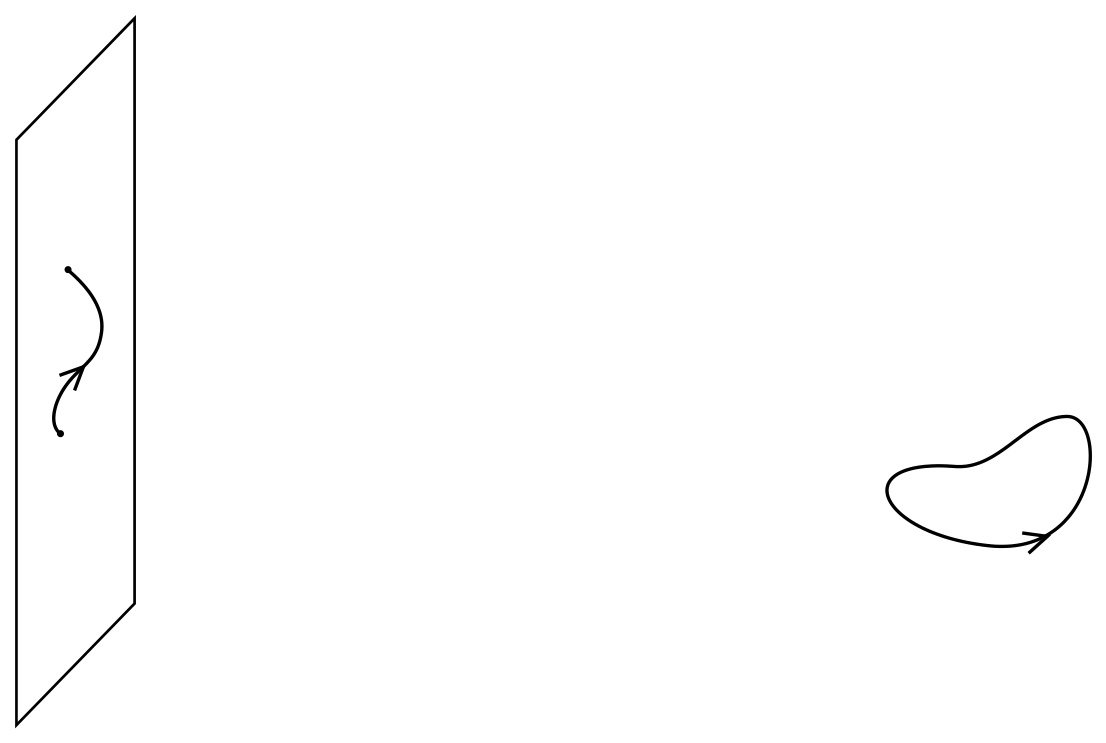
\includegraphics[width=0.65\textwidth]{figure/Fig13.1.jpg}
	\caption{A D-brane, with one attached open string and one closed string moving in the bulk. The physics away from the D-brane is described by a Type II string theory, so the string theory with the D-brane has the physical properties of a state of the Type II theory containing an extended object.}
	\label{fig:13.1}
\end{figure}

Now take the $R \to 0$ limit while concentrating on the neighborhood of one D-brane in the T-dual theory, adjusting the Wilson lines so that again the fixed plane and other D-branes move away in the T-dual spacetime. The low energy degrees of freedom on the D-brane are the massless open string states:
\begin{equation}
	\psi_{-1/2}^\mu\lvert k\rangle_{\mathrm{NS}} \:, \quad \psi_{-1/2}^9\lvert k\rangle_{\mathrm{NS}} \:, \quad \lvert \alpha; k\rangle_{\mathrm{R}} \:. \label{13.2.1}
\end{equation}
As in the bosonic theory, the bosonic states are a gauge field living on the D-brane and the collective coordinates for the D-brane. The fermionic states are the superpartners of these.

Consider now a process where closed strings scatter from the D-brane; this necessarily involves a worldsheet with boundary. Now, the open string boundary conditions are invariant only under $d = 10, N = 1$ supersymmetry. In the original Type I theory, the left-moving worldsheet current for spacetime supersymmetry $V_\alpha(z)$ flows into the boundary and the right-moving current $\tilde{V}_\alpha(\bar{z})$ flows out, so only the total charge $Q_\alpha + \tilde{Q}_\alpha$ of the left- and right-movers is conserved. Under T-duality this becomes:
\begin{equation}
	Q_\alpha' + (\beta_9\tilde{Q}')_\alpha \:. \label{13.2.2}
\end{equation}
The scattering amplitudes of closed strings from the D-brane are invariant only under these 16 supersymmetries.

To see the significance of this, consider first the conservation of momentum. There is a nonzero amplitude for a closed string to reflect backwards from the D-brane, which clearly does not conserve momentum in the direction orthogonal to the D-brane. This occurs because the Dirichlet boundary conditions explicitly break translational invariance. However, from the spacetime point of view the breaking is spontaneous: we are expanding around a D-brane in some definite location, but there are degenerate states with the D-brane translated by any amount (if the D-brane position were a fixed parameter in the Hamiltonian, translation invariance would be explicitly broken, but the D-brane position is a state label and not a parameter). For a spontaneously broken symmetry the consequences are more subtle than for an unbroken symmetry: the apparent violation of the conservation law is related to the amplitude to emit a long-wavelength Goldstone boson. For the D-brane, as for any extended object, the Goldstone bosons are the collective coordinates for its motion. In fact, the nonconservation of momentum is measured by the integral of the corresponding current over the worldsheet boundary:
\begin{equation}
	\frac{1}{2\pi\alpha'}\int_{\del\mathcal{M}}\dif s\:\del_n X'^9 \:, \label{13.2.3}
\end{equation}
which up to normalization is just the ($0$ picture) vertex operator for the collective coordinate, with zero momentum in the Neumann directions.

We conclude by analogy that the D-brane also spontaneously breaks 16 of the 32 spacetime supersymmetries, the ones that are explicitly broken by the open string boundary conditions. The integrals:
\begin{equation}
	\int_{\del\mathcal{M}}\dif s\:V_\alpha' = -\int_{\del\mathcal{M}}\dif s\:(\beta_9\tilde{V}')_\alpha \:, \label{13.2.4}
\end{equation}
which measure the breaking of supersymmetry, are just the vertex operators for the fermionic open string state \eqref{13.2.1}. Thus this state is a goldstino, the Goldstone state associated with spontaneously broken supersymmetry.
\begin{tcolorbox}[breakable]
	\begin{remark}
		\textbf{How a D-brane spontaneously breaks half of the 32 supersymmetries:
		the explicit calculation, from the world-sheet and from supergravity.}
		\medskip

The statement to be derived is that a D$p$-brane of type II string theory, extended along $X^1,\dots,X^p$, is an exact eigenstate of the 16 supercharges
\begin{equation}
Q_\alpha + (\beta^\perp \tilde Q)_\alpha , \qquad \beta^\perp = \beta^{p+1}\beta^{p+2}\cdots\beta^{9},
\tag{D.1}\label{unbroken}
\end{equation}
while the other 16 supercharges are broken spontaneously. Their failure to be conserved in any scattering amplitude equals the amplitude for emitting one extra massless open-string fermion at zero momentum, a goldstino. The derivation proceeds in five steps. A Ward identity on world-sheets with a boundary shows which charges a boundary condition preserves. T-duality turns the type I boundary condition into the D-brane boundary condition and fixes the matrices $\beta^m$. The same Ward identity then identifies the operator that measures the breaking, first for momentum and then for supersymmetry. The spacetime superalgebra shows that exactly 16 supercharges annihilate a brane that saturates the BPS bound. Finally, for the D3-brane, the Killing-spinor equation of type IIB supergravity on the extremal 3-brane solution reproduces the same 16 and the same projection. In every chain of equalities below, a numbered equality sign $\eqs{n}$ is explained in the sentence that follows the chain.

The metric is $\eta_{\mu\nu} = \mathrm{diag}(-1,1,\dots,1)$, the $32\times32$ Dirac matrices satisfy $\{\Gamma^\mu,\Gamma^\nu\} = 2\eta^{\mu\nu}$, and the chirality matrix is $\Gamma = \Gamma^0\Gamma^1\cdots\Gamma^9$. Its square is
\begin{align*}
\Gamma^2 &= (\Gamma^0\cdots\Gamma^9)(\Gamma^0\cdots\Gamma^9)
\eqs{1} (-1)^{45}(\Gamma^0\cdots\Gamma^9)(\Gamma^9\cdots\Gamma^0)\\
&\eqs{2} (-1)^{45}(\Gamma^0)^2(\Gamma^1)^2\cdots(\Gamma^9)^2 = (-1)(-1) = 1 .
\end{align*}
At (1) the second factor was reversed; reversing ten mutually anticommuting matrices takes $10\cdot9/2 = 45$ transpositions. At (2) the adjacent equal pairs were collapsed from the middle outwards. Moving any $\Gamma^\mu$ through $\Gamma$ passes nine anticommuting factors and one commuting factor, so $\Gamma\Gamma^\mu = -\Gamma^\mu\Gamma$. The real Clifford algebra of signature $(9,1)$ is the algebra of real $32\times32$ matrices, so there is a Majorana basis in which every $\Gamma^\mu$ is real. After an orthogonal change of basis, $\Gamma^0$ is antisymmetric and each $\Gamma^i$ is symmetric, and then $\Gamma$ is real and symmetric. The projectors $\frac12(1\pm\Gamma)$ have rank 16 each. The spacetime supersymmetry currents in the $-\frac12$ picture are $\mathcal V_\alpha = e^{-\phi/2}\Theta_\alpha$, holomorphic of weight $(1,0)$ with $\Theta_\alpha$ the spin field, and the antiholomorphic $\tilde{\mathcal V}_\alpha$. They are Hermitian in the Majorana basis and carry 16 real components of definite chirality. The charges
\begin{equation}
Q_\alpha = \frac{1}{2\pi i}\oint dz\,\mathcal V_\alpha , \qquad \tilde Q_\alpha = -\frac{1}{2\pi i}\oint d\bar z\,\tilde{\mathcal V}_\alpha
\tag{D.2}\label{charges}
\end{equation}
are contour independent. The minus sign compensates for $\oint d\bar z/\bar z = -2\pi i$, so that both charges measure a simple pole with the same sign.

Consider now a world-sheet with a boundary. The disk is represented as the upper half plane with its boundary on the real axis. Let $j(z)$ be holomorphic of weight $(1,0)$ and $\tilde j(\bar z)$ antiholomorphic of weight $(0,1)$, and write $\omega = dz\,j - d\bar z\,\tilde j$. The charge $\frac{1}{2\pi i}\oint\omega$ acts on a closed-string vertex operator at an interior point $z_i$ as $\delta V_i = \frac{1}{2\pi i}\oint_{z_i}\omega\,V_i$, the contour being a small counterclockwise circle around $z_i$. Take a disk amplitude with insertions $V_1,\dots,V_n$. Let $D$ be the upper half plane cut off at radius $R$, with small disks around the $z_i$ removed. Since $\omega$ is closed in $D$,
\begin{align*}
0 &= \frac{1}{2\pi i}\oint_{\partial D}\Big\langle \omega\, V_1\cdots V_n\Big\rangle \\
&\eqs{1} \frac{1}{2\pi i}\int_{-R}^{R}dx\,\Big\langle\big[j(x)-\tilde j(x)\big]V_1\cdots V_n\Big\rangle + \frac{1}{2\pi i}\int_{C_R}\Big\langle\omega\,V_1\cdots V_n\Big\rangle \\
&\quad - \sum_i\Big\langle V_1\cdots\delta V_i\cdots V_n\Big\rangle \\
&\eqs{2} \frac{1}{2\pi i}\int_{-\infty}^{\infty}dx\,\Big\langle\big[j(x)-\tilde j(x)\big]V_1\cdots V_n\Big\rangle - \sum_i\Big\langle V_1\cdots\delta V_i\cdots V_n\Big\rangle .
\end{align*}
At (1) the counterclockwise boundary of $D$ was split into three pieces. On the real axis $dz = d\bar z = dx$. The large semicircle $C_R$ remains. The small circles are traversed clockwise, which gives the minus sign. At (2), $R\to\infty$. On the disk the point at infinity is an ordinary boundary point. Under $w = -1/z$ a weight-$(1,0)$ field obeys $j(z) = (dw/dz)\,j(w) = z^{-2}j(w)$ with $j(w)$ regular at $w=0$, so $|\int_{C_R}dz\,j| \le \pi R\cdot R^{-2}\max|j(w)|\to0$, and likewise for $\tilde j$. The result is the Ward identity
\begin{equation}
\sum_{i=1}^n \Big\langle V_1\cdots \delta V_i \cdots V_n\Big\rangle = \frac{1}{2\pi i}\int_{-\infty}^{\infty} dx\,\Big\langle \big[j(x)-\tilde j(x)\big]\, V_1\cdots V_n\Big\rangle .
\tag{D.3}\label{ward}
\end{equation}
The charge is a symmetry of disk amplitudes exactly when $j=\tilde j$ on the boundary. Otherwise the right side is the boundary operator that measures the violation.

Apply this first to the momentum current $j = \frac{i}{\alpha'}\partial X^\mu$, $\tilde j = \frac{i}{\alpha'}\bar\partial X^\mu$, using the bulk propagator $X^\mu(z,\bar z)X^\nu(0)\sim -\frac{\alpha'}{2}\eta^{\mu\nu}\ln|z|^2$. The charge acts on a closed-string tachyon exponential as
\begin{align*}
j(z)\,e^{ik\cdot X}(0) &\eqs{1} \frac{i}{\alpha'}\,\partial_z\Big(-\frac{\alpha'}{2}\ln|z|^2\Big)\,ik^\mu\, e^{ik\cdot X}(0) = \frac{k^\mu}{2z}\,e^{ik\cdot X}(0), \\
\tilde j(\bar z)\,e^{ik\cdot X}(0) &= \frac{k^\mu}{2\bar z}\,e^{ik\cdot X}(0),\\
\delta\, e^{ik\cdot X} &= \frac{1}{2\pi i}\oint dz\,\frac{k^\mu}{2z}\,e^{ik\cdot X} - \frac{1}{2\pi i}\oint d\bar z\,\frac{k^\mu}{2\bar z}\,e^{ik\cdot X} \\
&\eqs{2} \Big(\frac{k^\mu}{2} + \frac{k^\mu}{2}\Big)e^{ik\cdot X} = k^\mu\,e^{ik\cdot X}.
\end{align*}
At (1) the single contraction of $\partial X^\mu$ with the exponential was taken. At (2) the residues $\oint dz/z = 2\pi i$ and $\oint d\bar z/\bar z = -2\pi i$ were used. On the real axis, with $\partial = \frac12(\partial_x - i\partial_y)$ and $\bar\partial = \frac12(\partial_x+i\partial_y)$,
\begin{align*}
j - \tilde j = \frac{i}{\alpha'}(\partial-\bar\partial)X^\mu = \frac{i}{\alpha'}(-i\,\partial_y)X^\mu = \frac{1}{\alpha'}\partial_yX^\mu ,
\end{align*}
so (\ref{ward}) becomes
\begin{equation}
\Big(\sum_i k_i^\mu\Big)\,A = \frac{1}{2\pi i\alpha'}\int dx\,\Big\langle \partial_y X^\mu(x)\,V_1\cdots V_n\Big\rangle ,
\tag{D.4}\label{momward}
\end{equation}
where $A$ is the amplitude. For Neumann conditions $\partial_yX^\mu = 0$ on the boundary, and momentum is conserved. For supersymmetry with a constant spinor $\epsilon^\alpha$, the charges (\ref{charges}) give, for the two combinations,
\begin{align*}
\epsilon\cdot(Q\pm\tilde Q) = \frac{1}{2\pi i}\oint\Big(dz\,\epsilon^\alpha\mathcal V_\alpha \mp d\bar z\,\epsilon^\alpha\tilde{\mathcal V}_\alpha\Big)
\quad\Longrightarrow\quad j - \tilde j\,\Big|_{\rm axis} = \epsilon^\alpha\big(\mathcal V_\alpha \mp \tilde{\mathcal V}_\alpha\big)(x).
\end{align*}
In the type I theory the Neumann conditions $\partial X^\mu = \bar\partial X^\mu$ and $\psi^\mu = \tilde\psi^\mu$ on the real axis make every right-moving field the image of a left-moving one, $\tilde\psi^\mu(\bar z) = \psi^\mu(z^*)$. The same holds for the superconformal ghosts, $\tilde\phi(\bar z) = \phi(z^*)$. After bosonization the spin field is an exponential of the bosons that bosonize pairs of $\psi^\mu$, so it inherits $\tilde\Theta_\alpha(\bar z) = \Theta_\alpha(z^*)$. Hence
\begin{equation}
\mathcal V_\alpha(x) = \tilde{\mathcal V}_\alpha(x)\qquad (x\ \text{real}),
\tag{D.5}\label{typeIbc}
\end{equation}
and both currents carry the same chirality. By (\ref{ward}), $Q+\tilde Q$ is a symmetry of every disk amplitude and $Q-\tilde Q$ is not; these are the 16 supercharges of type I.

T-duality in $X^9$ acts only on right-movers, $\partial X^9 \to \partial X'^9$ and $\bar\partial X^9 \to -\bar\partial X'^9$. On the real axis this gives
\begin{align*}
\partial_xX^9 &= (\partial+\bar\partial)X^9 \;\to\; (\partial-\bar\partial)X'^9 = -i\,\partial_yX'^9, \\
\partial_yX^9 &= i(\partial-\bar\partial)X^9 \;\to\; i(\partial+\bar\partial)X'^9 = i\,\partial_xX'^9 ,
\end{align*}
so the Neumann condition $\partial_yX^9 = 0$ becomes the Dirichlet condition $\partial_xX'^9 = 0$, and $X'^9$ sits at a fixed value $x^9$ on the boundary. The supercurrent $\tilde T_F\propto\tilde\psi_\mu\bar\partial X^\mu$ keeps its form only if $\tilde\psi^9\to-\tilde\psi^9$ as well. In the Ramond sector the zero modes obey $\{\tilde\psi^\mu_0,\tilde\psi^\nu_0\} = \eta^{\mu\nu}$ and act on the ground states $|\alpha\rangle\leftrightarrow\tilde\Theta_\alpha$ as $\Gamma^\mu/\sqrt2$. The reflection is therefore represented on them by a matrix $U$ with $U\Gamma^\mu U^{-1} = \Gamma^\mu$ for $\mu\ne9$ and $U\Gamma^9U^{-1} = -\Gamma^9$. The matrix $\beta^9 = \Gamma^9\Gamma$ satisfies this:
\begin{align*}
\beta^9\Gamma^\mu &= \Gamma^9\Gamma\Gamma^\mu \eqs{1} -\Gamma^9\Gamma^\mu\Gamma \eqs{2} \Gamma^\mu\Gamma^9\Gamma = \Gamma^\mu\beta^9 \qquad(\mu\neq9),\\
\beta^9\Gamma^9 &= \Gamma^9\Gamma\Gamma^9 \eqs{1} -\Gamma^9\Gamma^9\Gamma = -\Gamma^9\beta^9 .
\end{align*}
At (1), $\Gamma$ anticommutes with every $\Gamma^\mu$. At (2), $\Gamma^9$ anticommutes with $\Gamma^\mu$ for $\mu\ne9$. Any other solution $U$ makes $U^{-1}\beta^9$ commute with every $\Gamma^\mu$. The 32-dimensional representation is irreducible, so by Schur's lemma $U^{-1}\beta^9$ is a multiple of the identity and $U = \lambda\beta^9$. Hermiticity of the currents requires $U$ to be real, and preserving the normalization of the ground states requires it to be orthogonal. Both properties hold for $\beta^9$, which fixes $\lambda = \pm1$, and its square follows directly:
\begin{align*}
(\beta^9)^T\beta^9 &= \Gamma^T(\Gamma^9)^T\Gamma^9\Gamma \eqs{1} \Gamma\Gamma^9\Gamma^9\Gamma = 1, \\
\beta^9\beta^9 &= \Gamma^9\Gamma\Gamma^9\Gamma \eqs{2} -\Gamma^9\Gamma^9\Gamma\Gamma = -1, \\
\beta^9\Gamma &= \Gamma^9\Gamma\Gamma = \Gamma^9, \qquad \Gamma\beta^9 = \Gamma\Gamma^9\Gamma \eqs{2} -\Gamma^9 \quad\Longrightarrow\quad \beta^9\Gamma = -\Gamma\beta^9 .
\end{align*}
At (1), $\Gamma$ and $\Gamma^9$ are real and symmetric. At (2), $\Gamma$ anticommutes with $\Gamma^9$. Performing the duality twice therefore gives $-1$ on right-moving spinors, which is $\exp(\pi i\tilde F)$. The alternative $i\beta^9$ squares to $+1$ but is not real. The last line shows that $\beta^9$ flips chirality. The ghost factor $e^{-\tilde\phi/2}$ is unaffected by the duality.

Define the dual currents by $\mathcal V'_\alpha = \mathcal V_\alpha$ and $\tilde{\mathcal V}_\alpha = (\beta^9\tilde{\mathcal V}')_\alpha$, and the dual charges by (\ref{charges}). If $\Gamma\tilde Q = \tilde Q$, then
\begin{align*}
\Gamma\tilde Q' \eqs{1} \Gamma(-\beta^9\tilde Q) \eqs{2} \beta^9\Gamma\tilde Q = \beta^9\tilde Q \eqs{1} -\tilde Q' .
\end{align*}
At (1), $\tilde Q' = (\beta^9)^{-1}\tilde Q = -\beta^9\tilde Q$ because $(\beta^9)^2=-1$. At (2), $\beta^9$ anticommutes with $\Gamma$. The dual charges thus have opposite chirality, so the bulk theory is IIA. The boundary condition (\ref{typeIbc}) becomes
\begin{equation}
\mathcal V'_\alpha(x) = (\beta^9\tilde{\mathcal V}')_\alpha(x) \qquad (x\ \text{real}),
\tag{D.6}\label{dualbc}
\end{equation}
which is consistent because $\beta^9$ maps the chirality of $\tilde{\mathcal V}'$ to that of $\mathcal V'$. The constant matrix $\beta^9$ can be taken inside the contour integrals, so for the two combinations
\begin{align*}
\epsilon\cdot(Q'\pm\beta^9\tilde Q') &= \frac{1}{2\pi i}\oint\Big(dz\,\epsilon^\alpha\mathcal V'_\alpha \mp d\bar z\,\epsilon^\alpha(\beta^9\tilde{\mathcal V}')_\alpha\Big),\\
j-\tilde j\,\Big|_{\rm axis} &= \epsilon^\alpha\big(\mathcal V'_\alpha \mp (\beta^9\tilde{\mathcal V}')_\alpha\big)(x) \eqs{1}
\begin{cases} 0 & (+)\\ 2\epsilon^\alpha\mathcal V'_\alpha(x) & (-)\end{cases}
\end{align*}
where (1) uses (\ref{dualbc}). Inserting this into (\ref{ward}) gives
\begin{align}
\sum_i\Big\langle V_1\cdots\delta_{Q'+\beta^9\tilde Q'}V_i\cdots V_n\Big\rangle &= 0, \tag{D.7}\label{susyward1}\\
\sum_i\Big\langle V_1\cdots\delta_{Q'-\beta^9\tilde Q'}V_i\cdots V_n\Big\rangle &= \frac{1}{\pi i}\int dx\,\Big\langle \epsilon^\alpha\mathcal V'_\alpha(x)\,V_1\cdots V_n\Big\rangle . \tag{D.8}\label{susyward2}
\end{align}
Closed-string scattering off the D8-brane is therefore invariant under $Q'+\beta^9\tilde Q'$ but not under $Q'-\beta^9\tilde Q'$. Defining the dual current instead by $\tilde{\mathcal V}' = \beta^9\tilde{\mathcal V}$ interchanges the two, because $(\beta^9)^{-1} = -\beta^9$. The two choices describe a brane and an antibrane, which carry opposite Ramond--Ramond charge.

Whether the breaking in (\ref{susyward2}) is explicit or spontaneous is settled by first doing the same computation for momentum. In the dual variables the momentum current is $j = \frac{i}{\alpha'}\partial X'^9$, and (\ref{momward}) multiplied by $i$ reads
\begin{equation}
\Big\langle \frac{1}{2\pi\alpha'}\int dx\,\partial_y X'^9(x)\,V_1\cdots V_n\Big\rangle = i\Big(\sum_i k_i^9\Big)A ,
\tag{D.9}\label{dualmom}
\end{equation}
which does not vanish because $\partial_yX'^9\ne0$ on a Dirichlet boundary. Two facts identify the operator on the left. First, it is the T-dual of the zero-momentum vertex operator of the gauge field along 9. The 0-picture gauge-boson vertex operator is proportional to $\int dx\,(i\partial_xX^\mu + 2\alpha'k\cdot\psi\,\psi^\mu)e^{ik\cdot X}$, and
\begin{align*}
\int dx\,\big(i\partial_xX^9 + 2\alpha'k\cdot\psi\,\psi^9\big)e^{ik\cdot X}\Big|_{k=0}
= i\int dx\,\partial_xX^9 \;\to\; i\int dx\,(-i)\partial_yX'^9 = \int dx\,\partial_yX'^9 ,
\end{align*}
using the map of $\partial_xX^9$ derived above. The result is the zero-momentum vertex operator of the massless scalar that describes the transverse position of the brane. Second, it generates translations of the brane. Write $X'^9 = x^9 + Y$ with $Y=0$ on the boundary; then
\begin{align*}
A(x^9) = \int\mathcal DX'\,e^{-S[X']}\prod_i e^{ik_i\cdot X'}
&\eqs{1} \int\mathcal DY\,e^{-S[Y]}\prod_i e^{ik_i^9x^9}e^{ik_i\cdot Y} = e^{ix^9\sum_ik_i^9}A(0), \\
\frac{\partial A}{\partial x^9} &= i\Big(\sum_ik_i^9\Big)A \eqs{2} \Big\langle\frac{1}{2\pi\alpha'}\int dx\,\partial_yX'^9(x)\,V_1\cdots V_n\Big\rangle .
\end{align*}
At (1), the free action depends only on derivatives of $X'$, the measure is shift invariant, and the exponentials factorize. At (2), (\ref{dualmom}) was used. The non-conservation of momentum is thus the amplitude to emit a zero-momentum quantum of the collective coordinate, and inserting that quantum moves the brane infinitesimally. This is the structure of a spontaneously broken symmetry. The ground state, the brane at $x^9$, is not invariant but belongs to a degenerate family of translated ground states. The apparent violation of the conservation law is the emission of the long-wavelength Goldstone mode that moves the system along that family.

Equation (\ref{susyward2}) has the same structure. The massless open-string Ramond state $|\alpha;k\rangle_{\rm R}$ has the $-\frac12$-picture boundary vertex operator $u^\alpha e^{-\phi/2}\Theta_\alpha e^{ik\cdot X}$, subject to $k^2 = 0$ and $k_\mu\Gamma^\mu u = 0$. At $k=0$ both conditions hold trivially, and $\int dx\,\epsilon^\alpha\mathcal V'_\alpha = \int dx\,\epsilon^\alpha e^{-\phi/2}\Theta_\alpha$ is this vertex operator with $u = \epsilon$. The GSO projection keeps $u$ in the chirality of $\mathcal V'$. The variation of any closed-string amplitude under a broken supersymmetry is therefore $1/(\pi i)$ times the amplitude with one extra zero-momentum open-string fermion. That fermion is the goldstino, and the 16 supersymmetries broken explicitly by the world-sheet boundary condition are broken spontaneously in spacetime.

The count of 16 and 16 is exact. The change of basis from $(Q',\tilde Q')$ to $Q'\pm\beta^9\tilde Q'$ is the matrix $\begin{pmatrix}1&\beta^9\\1&-\beta^9\end{pmatrix}$, which is invertible because $\beta^9$ is. The new charges are Hermitian because $\beta^9$ is real, and each set has 16 components in the chiral subspace of $Q'$. For a D$p$-brane, T-dualize $X^{p+1},\dots,X^9$ in turn. Each duality multiplies the right-moving spinor by one more $\beta^m$, the boundary condition becomes $\mathcal V' = \beta^\perp\tilde{\mathcal V}'$, and the argument from (\ref{dualbc}) to (\ref{susyward2}) goes through unchanged with $\beta^\perp$ in place of $\beta^9$. The unbroken charges are then (\ref{unbroken}). The properties of $\beta^\perp$ follow from
\begin{align*}
\beta^m\beta^n = \Gamma^m\Gamma\Gamma^n\Gamma \eqs{1} -\Gamma^m\Gamma^n\Gamma\Gamma = -\Gamma^m\Gamma^n \eqs{2} \Gamma^n\Gamma^m = -\beta^n\beta^m \qquad (m\ne n),
\end{align*}
where (1) uses $\Gamma\Gamma^n = -\Gamma^n\Gamma$ and (2) uses $\Gamma^m\Gamma^n = -\Gamma^n\Gamma^m$; the final step reads the first two equalities backwards with $m\leftrightarrow n$. Thus the order of the dualities changes $\beta^\perp$ only by a sign, which is again the brane versus antibrane choice. With $n = 9-p$ factors,
\begin{align}
(\beta^\perp)^2 = (\beta^{p+1}\cdots\beta^9)(\beta^{p+1}\cdots\beta^9)
&\eqs{1} (-1)^{n(n-1)/2}(\beta^{p+1}\cdots\beta^9)(\beta^9\cdots\beta^{p+1}) \notag\\
&\eqs{2} (-1)^{n(n-1)/2}(-1)^{n} = (-1)^{(9-p)(10-p)/2}. \tag{D.10}\label{bsq}
\end{align}
At (1) the second product was reversed, which takes $n(n-1)/2$ transpositions of anticommuting factors. At (2) the product collapses from the middle using $(\beta^m)^2 = -1$. The matrix $\beta^\perp$ is also real and orthogonal, as a product of real orthogonal matrices, and $\beta^\perp\Gamma = (-1)^{9-p}\Gamma\beta^\perp$ because each factor anticommutes with $\Gamma$. The boundary condition relates currents of opposite chirality in IIA and of the same chirality in IIB. It is therefore consistent for even $p$ in IIA and odd $p$ in IIB.

Next, the superalgebra. Taken as input, with Hermitian charges in the Majorana basis, it reads
\begin{align}
\{Q_\alpha,Q_\beta^\dagger\} &= 2\Big[P_M + \frac{Q^{\rm NS}_M}{2\pi\alpha'}\Big](\Gamma^0\Gamma^M)_{\alpha\beta}, \notag\\
\{\tilde Q_\alpha,\tilde Q_\beta^\dagger\} &= 2\Big[P_M - \frac{Q^{\rm NS}_M}{2\pi\alpha'}\Big](\Gamma^0\Gamma^M)_{\alpha\beta}, \tag{D.11}\label{alg1}\\
\{Q_\alpha,\tilde Q_\beta^\dagger\} &= 2\sum_p\frac{\tau_p}{p!}\,Q^{\rm R}_{M_1\cdots M_p}\,(\beta^{M_1}\cdots\beta^{M_p}\Gamma^0)_{\alpha\beta}. \tag{D.12}\label{alg2}
\end{align}
For a static D$p$-brane along $X^1,\dots,X^p$ in its rest frame, $P_0 = -E$, $P_i = 0$ and $Q^{\rm NS} = 0$. Writing $Z = \tau_pQ^{\rm R}_{1\cdots p}$ and $M = \beta^1\cdots\beta^p\Gamma^0$,
\begin{align*}
\{Q_\alpha,Q_\beta^\dagger\} &= 2P_0(\Gamma^0\Gamma^0)_{\alpha\beta} = 2(-E)(-1)\delta_{\alpha\beta} \\
&= 2E\,\delta_{\alpha\beta} = \{\tilde Q_\alpha,\tilde Q_\beta^\dagger\}, \\
\{Q_\alpha,\tilde Q_\beta^\dagger\} &\eqs{1} \frac{2\tau_p}{p!}\sum_{\sigma\in S_p}Q^{\rm R}_{\sigma(1)\cdots\sigma(p)}\big(\beta^{\sigma(1)}\cdots\beta^{\sigma(p)}\Gamma^0\big)_{\alpha\beta}\\
&\eqs{2} \frac{2\tau_p}{p!}\sum_{\sigma\in S_p}(\mathrm{sgn}\,\sigma)^2\,Q^{\rm R}_{1\cdots p}\,M_{\alpha\beta} = 2Z\,M_{\alpha\beta}, \\
\{\tilde Q_\beta,Q_\alpha^\dagger\} &\eqs{3} \big(\{Q_\alpha,\tilde Q_\beta^\dagger\}\big)^\dagger = 2Z\,M^*_{\alpha\beta} = 2Z\,M_{\alpha\beta} .
\end{align*}
At (1) only permutations of $(1,\dots,p)$ contribute to the index sum. At (2) the charge and the product of anticommuting $\beta$'s each change by $\mathrm{sgn}\,\sigma$ under reordering. At (3), $(AB+BA)^\dagger = B^\dagger A^\dagger + A^\dagger B^\dagger$, and $M$ is real. For $Q_\pm = Q\pm\beta^\perp\tilde Q$, the reality of $\beta^\perp$ gives $(\beta^\perp\tilde Q)^\dagger_\beta = \beta^\perp_{\beta\delta}\tilde Q^\dagger_\delta$, and
\begin{align*}
\{Q_{\pm\alpha},Q_{\pm\beta}^\dagger\}
&= \{Q_\alpha,Q_\beta^\dagger\} + \beta^\perp_{\alpha\gamma}\beta^\perp_{\beta\delta}\{\tilde Q_\gamma,\tilde Q_\delta^\dagger\} \\
&\quad \pm \beta^\perp_{\beta\delta}\{Q_\alpha,\tilde Q_\delta^\dagger\} \pm \beta^\perp_{\alpha\gamma}\{\tilde Q_\gamma,Q_\beta^\dagger\} \\
&= 2E\,\delta_{\alpha\beta} + 2E\,\big(\beta^\perp(\beta^\perp)^T\big)_{\alpha\beta} \\
&\quad \pm 2Z\,\big(M(\beta^\perp)^T\big)_{\alpha\beta} \pm 2Z\,\big(\beta^\perp M^T\big)_{\alpha\beta} \\
&\eqs{1} 4E\,\delta_{\alpha\beta} \pm 2Z\Big[M(\beta^\perp)^T + \big(M(\beta^\perp)^T\big)^T\Big]_{\alpha\beta} .
\end{align*}
At (1), $\beta^\perp$ is orthogonal. The matrix in the bracket is evaluated with two identities. The first is that $\Gamma^0$ commutes with each spatial $\beta^m$, since $\Gamma^0\Gamma^m\Gamma = -\Gamma^m\Gamma^0\Gamma = \Gamma^m\Gamma\Gamma^0$. The second is
\begin{align*}
\beta^1\beta^2\cdots\beta^9 &= (\Gamma^1\Gamma\,\Gamma^2\Gamma)(\Gamma^3\Gamma\,\Gamma^4\Gamma)(\Gamma^5\Gamma\,\Gamma^6\Gamma)(\Gamma^7\Gamma\,\Gamma^8\Gamma)\,\Gamma^9\Gamma \\
&\eqs{1} (-1)^4\,\Gamma^1\Gamma^2\cdots\Gamma^9\,\Gamma \eqs{2} -\Gamma^0\Gamma\Gamma = -\Gamma^0 .
\end{align*}
At (1) each pair is $\Gamma^m\Gamma\Gamma^n\Gamma = -\Gamma^m\Gamma^n$. At (2), $\Gamma^0\Gamma = (\Gamma^0)^2\Gamma^1\cdots\Gamma^9 = -\Gamma^1\cdots\Gamma^9$. With these,
\begin{align*}
M(\beta^\perp)^T = \beta^1\cdots\beta^p\,\Gamma^0\,(\beta^\perp)^T
&\eqs{1} -\Gamma^0(\beta^\perp)^{-1}\,\Gamma^0\,(\beta^\perp)^{-1}\\
&\eqs{2} -(\Gamma^0)^2(\beta^\perp)^{-2} = (\beta^\perp)^{-2} \eqs{3} (-1)^{(9-p)(10-p)/2} \equiv c .
\end{align*}
At (1), $\beta^1\cdots\beta^p = (\beta^1\cdots\beta^9)(\beta^\perp)^{-1} = -\Gamma^0(\beta^\perp)^{-1}$ and $(\beta^\perp)^T = (\beta^\perp)^{-1}$. At (2), $\Gamma^0$ was moved through $(\beta^\perp)^{-1}$. At (3), equation (\ref{bsq}) was used together with $c^{-1} = c$. Since the bracket is $2c$ times the identity,
\begin{equation}
\{Q_{\pm\alpha},Q_{\pm\beta}^\dagger\} = 4\,(E \pm cZ)\,\delta_{\alpha\beta}.
\tag{D.13}\label{bps}
\end{equation}
The consequences follow by taking expectation values in the brane state $|B\rangle$. For Hermitian $Q_{\pm\alpha}$, $\langle B|\{Q_{\pm\alpha},Q_{\pm\alpha}\}|B\rangle = 2\|Q_{\pm\alpha}|B\rangle\|^2 = 4(E\pm cZ)\langle B|B\rangle$. Positivity for both signs gives the BPS bound $E\ge|Z|$. If all 16 components of $Q_+$ annihilate $|B\rangle$, then $E = -cZ$ and the bound is saturated. In that case $2\|Q_{-\alpha}|B\rangle\|^2 = 8E\langle B|B\rangle > 0$, so no component of $Q_-$ annihilates the brane. A state annihilated by all 32 supercharges would need $E = cZ = -cZ$, i.e.\ $E = 0$, which is the vacuum. The conclusion uses only the fact that $M(\beta^\perp)^T$ is $\pm1$ times the identity, not the normalization of $Z$ or the sign $c$.

The same 16 supersymmetries follow from type IIB supergravity on the extremal D3-brane. In a bosonic background the fermions vanish, so a supersymmetry preserves the background exactly when the fermion variations vanish. The dilatino variation is built from the gradient of the axion-dilaton and from the three-form field strengths, all of which vanish for the D3-brane, so it is identically zero. What remains is the gravitino condition. The following IIB conventions are taken as input. The parameter $\epsilon$ is a complex Weyl spinor with $\Gamma\epsilon=\epsilon$, and
\begin{align}
\delta\psi_M &= \nabla_M\epsilon + \frac{i}{16}\,\slashed F\,\Gamma_M\,\epsilon, \notag\\
R_{MN} &= \frac{1}{96}F_{MPQRS}F_N{}^{PQRS}, \qquad F = *F ,
\tag{D.14}\label{iib}
\end{align}
with $\slashed F = \frac{1}{5!}F_{N_1\cdots N_5}\Gamma^{N_1\cdots N_5}$ and $\nabla_M\epsilon = \partial_M\epsilon + \frac14\omega_{M\hat A\hat B}\Gamma^{\hat A}\Gamma^{\hat B}\epsilon$. Hatted indices are flat, $\Gamma_M = e^{\hat A}{}_M\Gamma_{\hat A}$, and the Hodge dual uses $\epsilon_{\hat0\hat1\cdots\hat9} = +1$. The relative normalization in $\delta\psi_M$ is fixed by IIB supersymmetry and is not derived here. The extremal D3-brane along $x^0,\dots,x^3$, with transverse coordinates $y^4,\dots,y^9$, is
\begin{align}
ds^2 &= H^{-1/2}\eta_{ab}\,dx^a dx^b + H^{1/2}\,dy^i dy^i, \notag\\
F &= (1+*)\,d\big(H^{-1}\big)\wedge dx^0\wedge dx^1\wedge dx^2\wedge dx^3 ,
\tag{D.15}\label{d3sol}
\end{align}
where $a,b$ run over $0,\dots,3$, $i$ runs over $4,\dots,9$, and $H = 1+L^4/r^4$ with $r^2 = y^iy^i$. The electric components are $F_{i0123} = \partial_i(H^{-1}) = -H^{-2}\partial_iH$, and $H$ is harmonic away from $r=0$:
\begin{align*}
\partial_i\partial_i\, r^n = \partial_i\big(n\,r^{n-2}y^i\big) = n\big[(n-2)r^{n-4}y^iy^i + 6\,r^{n-2}\big] = n(n+4)\,r^{n-2} \;\xrightarrow{\;n=-4\;}\; 0 .
\end{align*}
The configuration (\ref{d3sol}) is the standard extremal solution of the field equations in (\ref{iib}), and it is taken as given here.

Write $H^{-1/2} = e^{2A}$ and $H^{1/2} = e^{2B}$, so $A = -\frac14\ln H$ and $B = \frac14\ln H$, and use the vielbein $e^{\hat a} = e^Adx^a$, $e^{\hat i} = e^Bdy^i$. Cartan's equation $de^{\hat A} = -\omega^{\hat A}{}_{\hat B}\wedge e^{\hat B}$ is solved by $\omega^{\hat a}{}_{\hat i} = e^{-B}\partial_iA\,e^{\hat a}$, $\omega^{\hat i}{}_{\hat j} = e^{-B}(\partial_jB\,e^{\hat i}-\partial_iB\,e^{\hat j})$ and $\omega^{\hat a}{}_{\hat b} = 0$. To verify this, compute
\begin{align*}
de^{\hat a} &= \partial_iA\,e^A\,dy^i\wedge dx^a = \partial_iA\,e^{-B}\,e^{\hat i}\wedge e^{\hat a}, \\
-\omega^{\hat a}{}_{\hat i}\wedge e^{\hat i} &= -e^{-B}\partial_iA\,e^{\hat a}\wedge e^{\hat i} = \partial_iA\,e^{-B}\,e^{\hat i}\wedge e^{\hat a}, \\
de^{\hat i} &= \partial_jB\,e^B\,dy^j\wedge dy^i = \partial_jB\,e^{-B}\,e^{\hat j}\wedge e^{\hat i}, \\
-\omega^{\hat i}{}_{\hat j}\wedge e^{\hat j} &= -e^{-B}\partial_jB\,e^{\hat i}\wedge e^{\hat j} + e^{-B}\partial_iB\,e^{\hat j}\wedge e^{\hat j} = \partial_jB\,e^{-B}\,e^{\hat j}\wedge e^{\hat i} ,
\end{align*}
and note that $\omega^{\hat i}{}_{\hat a}\wedge e^{\hat a} = 0$ because $\omega^{\hat i}{}_{\hat a}\propto e^{\hat a}$. Reading off components with both flat indices lowered gives
\begin{equation*}
\omega_{a\,\hat a\hat i} = \eta_{aa}\,e^{A-B}\partial_iA\ \ (\text{no sum}), \qquad
\omega_{k\,\hat i\hat j} = \partial_jB\,\delta_{ki} - \partial_iB\,\delta_{kj} ,
\end{equation*}
For $\epsilon = f(y)\epsilon_0$ with $\epsilon_0$ constant, the covariant derivatives are
\begin{align*}
\nabla_a\epsilon &= \frac14\big(\omega_{a\hat a\hat i}\Gamma^{\hat a}\Gamma^{\hat i} + \omega_{a\hat i\hat a}\Gamma^{\hat i}\Gamma^{\hat a}\big)\epsilon
\eqs{1} \frac12\,\omega_{a\hat a\hat i}\Gamma^{\hat a}\Gamma^{\hat i}\epsilon\\
&\eqs{2} \frac12\,e^{A-B}\partial_iA\,\Gamma_{\hat a}\Gamma^{\hat i}\epsilon
\eqs{3} -\frac18\,H^{-3/2}\partial_iH\,\Gamma_{\hat a}\Gamma^{\hat i}\epsilon , \\
\nabla_k\epsilon &= \partial_kf\,\epsilon_0 + \frac14\sum_{i,j}\big(\partial_jB\,\delta_{ki}-\partial_iB\,\delta_{kj}\big)\Gamma^{\hat i}\Gamma^{\hat j}\epsilon\\
&= \partial_kf\,\epsilon_0 + \frac14\Big(\sum_j\partial_jB\,\Gamma^{\hat k}\Gamma^{\hat j} - \sum_i\partial_iB\,\Gamma^{\hat i}\Gamma^{\hat k}\Big)\epsilon \\
&\eqs{4} \partial_kf\,\epsilon_0 + \frac12\sum_{j\ne k}\partial_jB\,\Gamma^{\hat k}\Gamma^{\hat j}\epsilon
\eqs{3} \partial_kf\,\epsilon_0 + \frac18 fH^{-1}\sum_{j\ne k}\partial_jH\,\Gamma^{\hat k}\Gamma^{\hat j}\epsilon_0 .
\end{align*}
At (1), $\omega_{a\hat i\hat a} = -\omega_{a\hat a\hat i}$ and $\Gamma^{\hat i}\Gamma^{\hat a} = -\Gamma^{\hat a}\Gamma^{\hat i}$, and $\partial_a\epsilon = 0$. At (2), $\eta_{aa}\Gamma^{\hat a} = \Gamma_{\hat a}$. At (3), $e^{A-B} = H^{-1/2}$, $\partial_iA = -\frac14H^{-1}\partial_iH$ and $\partial_jB = \frac14H^{-1}\partial_jH$. At (4), the $j=k$ and $i=k$ terms are both $\partial_kB$ and cancel, and $\Gamma^{\hat j}\Gamma^{\hat k} = -\Gamma^{\hat k}\Gamma^{\hat j}$ for $j\ne k$.

The flux term needs $\slashed F$. Its electric part is
\begin{align*}
F_{\hat i\hat0\hat1\hat2\hat3} &= e^{-B}e^{-4A}F_{i0123} = H^{-1/4}H^{+1}\big(-H^{-2}\partial_iH\big) = -H^{-5/4}\partial_iH, \\
\slashed F_{\rm el} & \eqs{1} \sum_i F_{\hat0\hat1\hat2\hat3\hat i}\,\Gamma^{\hat0\hat1\hat2\hat3}\Gamma^{\hat i} \eqs{2} -H^{-5/4}\partial_iH\,\Gamma^{\hat0\hat1\hat2\hat3}\Gamma^{\hat i} .
\end{align*}
At (1), each unordered index set appears $5!$ times in the sum, which cancels the $\frac{1}{5!}$. At (2), moving $\hat i$ past four indices is an even permutation. The magnetic part uses the identity
\begin{equation*}
\Gamma^{A_1\cdots A_5}\,\Gamma = \frac{1}{5!}\,\epsilon^{A_1\cdots A_5B_1\cdots B_5}\,\Gamma_{B_1\cdots B_5}.
\end{equation*}
It states that multiplying five distinct gamma matrices by $\Gamma$ leaves the complementary five. To prove it, fix distinct $A_1,\dots,A_5$ and let $B_1<\dots<B_5$ be the remaining indices. Then
\begin{align*}
\Gamma^{A_1\cdots A_5}\,\Gamma &\eqs{1} \epsilon_{A_1\cdots A_5B_1\cdots B_5}\,\Gamma^{A_1\cdots A_5}\Gamma^{A_1\cdots A_5}\Gamma^{B_1\cdots B_5}
\eqs{2} \epsilon_{A_1\cdots A_5B_1\cdots B_5}\,\eta^{A_1A_1}\cdots\eta^{A_5A_5}\,\Gamma^{B_1\cdots B_5} \\
&\eqs{3} \epsilon_{A_1\cdots A_5B_1\cdots B_5}\,\eta^{A_1A_1}\cdots\eta^{A_5A_5}\,\eta^{B_1B_1}\cdots\eta^{B_5B_5}\,\Gamma_{B_1\cdots B_5} \\
&\eqs{4} -\epsilon_{A_1\cdots A_5B_1\cdots B_5}\,\Gamma_{B_1\cdots B_5}
\eqs{5} \epsilon^{A_1\cdots A_5B_1\cdots B_5}\,\Gamma_{B_1\cdots B_5} .
\end{align*}
At (1), $\Gamma = \Gamma^0\cdots\Gamma^9$ was reordered into the order $A_1\cdots A_5B_1\cdots B_5$; for mutually anticommuting factors this costs the sign of the permutation, which is $\epsilon_{A_1\cdots A_5B_1\cdots B_5}$. At (2), the second $\Gamma^{A_1\cdots A_5}$ was reversed, which costs $(-1)^{10} = +1$, and the product was collapsed using $(\Gamma^{A})^2 = \eta^{AA}$. At (3), $\Gamma^{B} = \eta^{BB}\Gamma_{B}$. At (4), the product of all ten diagonal entries of $\eta$ is $-1$. At (5), raising all ten indices of $\epsilon$ produces the same factor $-1$. In the identity the sum over the $5!$ orderings of $B_1\cdots B_5$ gives $5!$ equal terms, which the $\frac{1}{5!}$ cancels. Then
\begin{align*}
\slashed F_{\rm mag} &= \frac{1}{5!}(*F)_{A_1\cdots A_5}\Gamma^{A_1\cdots A_5}
= \frac{1}{5!\,5!}\,\epsilon_{A_1\cdots A_5B_1\cdots B_5}F^{B_1\cdots B_5}\,\Gamma^{A_1\cdots A_5} \\
&\eqs{1} -\frac{1}{5!}F^{B_1\cdots B_5}\,\frac{1}{5!}\,\epsilon_{B_1\cdots B_5}{}^{A_1\cdots A_5}\Gamma_{A_1\cdots A_5}
\eqs{2} -\frac{1}{5!}F^{B_1\cdots B_5}\,\Gamma_{B_1\cdots B_5}\Gamma = -\slashed F_{\rm el}\,\Gamma ,
\end{align*}
so that
\begin{align*}
\slashed F &= \slashed F_{\rm el}(1-\Gamma), \\
\slashed F\,\Gamma_M\epsilon &= \slashed F_{\rm el}\big(\Gamma_M\epsilon - \Gamma\Gamma_M\epsilon\big) \eqs{3} \slashed F_{\rm el}\big(\Gamma_M\epsilon + \Gamma_M\Gamma\epsilon\big) = 2\slashed F_{\rm el}\,\Gamma_M\epsilon .
\end{align*}
At (1) the two blocks of five indices in $\epsilon$ were exchanged, which costs $(-1)^{25} = -1$, and the contracted $A$ indices were moved from $\Gamma$ to $\epsilon$. At (2) the identity above was applied with its free indices lowered. At (3), $\Gamma$ anticommutes with $\Gamma_M$ and $\Gamma\epsilon = \epsilon$. For a parameter of the other chirality the flux term would vanish and the equations below would force $\epsilon = 0$, so the chirality of $\epsilon$ is tied to the self-duality of $F$.

Along the brane $\Gamma_a = H^{-1/4}\Gamma_{\hat a}$, and
\begin{align*}
\delta\psi_a &= f\Big[-\frac18H^{-3/2}\partial_iH\,\Gamma_{\hat a}\Gamma^{\hat i} + \frac{i}{16}\cdot2\slashed F_{\rm el}\,H^{-1/4}\Gamma_{\hat a}\Big]\epsilon_0 \\
&= f\Big[-\frac18H^{-3/2}\partial_iH\,\Gamma_{\hat a}\Gamma^{\hat i} - \frac{i}{8}H^{-3/2}\partial_iH\,\Gamma^{\hat0\hat1\hat2\hat3}\Gamma^{\hat i}\Gamma_{\hat a}\Big]\epsilon_0 \\
&\eqs{1} f\Big[-\frac18H^{-3/2}\partial_iH\,\Gamma_{\hat a}\Gamma^{\hat i} - \frac{i}{8}H^{-3/2}\partial_iH\,\Gamma_{\hat a}\Gamma^{\hat i}\Gamma^{\hat0\hat1\hat2\hat3}\Big]\epsilon_0 \\
&= -\frac18fH^{-3/2}\partial_iH\,\Gamma_{\hat a}\Gamma^{\hat i}\big(1+i\,\Gamma^{\hat0\hat1\hat2\hat3}\big)\epsilon_0 .
\end{align*}
At (1) the chain $\Gamma^{\hat0\hat1\hat2\hat3}\Gamma^{\hat i}\Gamma_{\hat a} = -\Gamma^{\hat0\hat1\hat2\hat3}\Gamma_{\hat a}\Gamma^{\hat i} = \Gamma_{\hat a}\Gamma^{\hat0\hat1\hat2\hat3}\Gamma^{\hat i} = \Gamma_{\hat a}\Gamma^{\hat i}\Gamma^{\hat0\hat1\hat2\hat3}$ was used. Here $\Gamma^{\hat0\hat1\hat2\hat3}$ anticommutes with $\Gamma_{\hat a}$, since it contains $\Gamma_{\hat a}$ once among three other factors, and commutes with $\Gamma^{\hat i}$, which anticommutes with all four factors. The prefactor $\Gamma_{\hat a}\,\partial_iH\,\Gamma^{\hat i}$ is invertible wherever $\partial H\ne0$, since its square is $-(\Gamma_{\hat a})^2(\partial_iH\,\Gamma^{\hat i})^2 = -\eta_{aa}\,\partial_iH\partial_iH$. The condition $\delta\psi_a=0$ is therefore
\begin{equation}
\big(1+i\,\Gamma^{\hat0\hat1\hat2\hat3}\big)\epsilon_0 = 0 \quad\Longleftrightarrow\quad \Gamma^{\hat0\hat1\hat2\hat3}\,\epsilon_0 = i\,\epsilon_0 ,
\tag{D.16}\label{d3proj}
\end{equation}
the projection of the D3-brane, and it places no condition on $f$. The eigenvalue is $i$ rather than $\pm1$ because
\begin{align*}
(\Gamma^{\hat0\hat1\hat2\hat3})^2 = \Gamma^{\hat0}\Gamma^{\hat1}\Gamma^{\hat2}\Gamma^{\hat3}\Gamma^{\hat0}\Gamma^{\hat1}\Gamma^{\hat2}\Gamma^{\hat3}
\eqs{1} -(\Gamma^{\hat0})^2\,\Gamma^{\hat1}\Gamma^{\hat2}\Gamma^{\hat3}\Gamma^{\hat1}\Gamma^{\hat2}\Gamma^{\hat3}
\eqs{2} \Gamma^{\hat2}\Gamma^{\hat3}\Gamma^{\hat2}\Gamma^{\hat3}
\eqs{3} -1 .
\end{align*}
At (1) the second $\Gamma^{\hat0}$ was moved left past three factors. At (2), $(\Gamma^{\hat0})^2 = -1$, and $\Gamma^{\hat1}$ was moved past two factors and squared to $+1$. At (3), $\Gamma^{\hat2}$ was moved past one factor. The form $\Gamma^{01\cdots p}\epsilon_0 = \pm\epsilon_0$ often quoted for general $p$ cannot hold literally for the D3-brane.

In the transverse directions $\Gamma_k = H^{1/4}\Gamma_{\hat k}$, and the flux term reduces, using (\ref{d3proj}), to
\begin{align*}
\frac{i}{16}\cdot2\slashed F_{\rm el}H^{1/4}\Gamma_{\hat k}\,f\epsilon_0
&= -\frac{i}{8}fH^{-1}\partial_jH\,\Gamma^{\hat0\hat1\hat2\hat3}\Gamma^{\hat j}\Gamma^{\hat k}\epsilon_0
\eqs{1} -\frac{i}{8}fH^{-1}\partial_jH\,\Gamma^{\hat j}\Gamma^{\hat k}\,\Gamma^{\hat0\hat1\hat2\hat3}\epsilon_0 \\
&\eqs{2} \frac18fH^{-1}\sum_j\partial_jH\,\Gamma^{\hat j}\Gamma^{\hat k}\epsilon_0 \\
&\eqs{3} \frac18fH^{-1}\Big(\partial_kH - \sum_{j\ne k}\partial_jH\,\Gamma^{\hat k}\Gamma^{\hat j}\Big)\epsilon_0 .
\end{align*}
At (1), $\Gamma^{\hat0\hat1\hat2\hat3}$ commutes with transverse gamma matrices. At (2), (\ref{d3proj}) gives the factor $-\frac{i}{8}\cdot i = \frac18$. At (3) the $j=k$ term was separated and $\Gamma^{\hat j}\Gamma^{\hat k} = -\Gamma^{\hat k}\Gamma^{\hat j}$ was used for $j\ne k$. Adding $\nabla_k\epsilon$,
\begin{align*}
\delta\psi_k &= \partial_kf\,\epsilon_0 + \frac18fH^{-1}\sum_{j\ne k}\partial_jH\,\Gamma^{\hat k}\Gamma^{\hat j}\epsilon_0 \\
&\quad + \frac18fH^{-1}\Big(\partial_kH - \sum_{j\ne k}\partial_jH\,\Gamma^{\hat k}\Gamma^{\hat j}\Big)\epsilon_0 \\
&= \Big(\partial_kf + \frac18fH^{-1}\partial_kH\Big)\epsilon_0 ,
\end{align*}
so $\delta\psi_k = 0$ requires $\partial_k\ln f = -\frac18\partial_k\ln H$, that is $f = H^{-1/8}$ up to a constant absorbed into $\epsilon_0$. The Killing spinors are therefore $\epsilon = H^{-1/8}\epsilon_0$ with $\Gamma\epsilon_0 = \epsilon_0$ and (\ref{d3proj}). Reversing the sign of $F$ (the antibrane) reverses the flux term, so the brane condition becomes $(1 - i\Gamma^{\hat0\hat1\hat2\hat3})\epsilon_0 = 0$ and selects the eigenvalue $-i$.

The count is 16. The matrix $\Gamma^{\hat0\hat1\hat2\hat3}$ is real and commutes with $\Gamma$, so it acts within the 16 complex components of a Weyl spinor. There it squares to $-1$ and is traceless, since $\mathrm{tr}\big[\frac12(1+\Gamma)\Gamma^{\hat0\hat1\hat2\hat3}\big] = \frac12\mathrm{tr}\,\Gamma^{\hat0\hat1\hat2\hat3} + \frac12\mathrm{tr}\,\Gamma^{\hat0\hat1\hat2\hat3}\Gamma = 0$, both being products of distinct gamma matrices. Its eigenvalues $\pm i$ therefore each occur 8 times, and (\ref{d3proj}) keeps 8 complex, or 16 real, of the 32 supersymmetries. To compare with the world-sheet result, identify $\epsilon = \epsilon_L + i\epsilon_R$ in terms of the Majorana--Weyl parameters that multiply $Q$ and $\tilde Q$; this identification is a convention. Since $\Gamma^{\hat0\hat1\hat2\hat3}$ is real,
\begin{align*}
\Gamma^{\hat0\hat1\hat2\hat3}\epsilon_L + i\,\Gamma^{\hat0\hat1\hat2\hat3}\epsilon_R = i\epsilon_L - \epsilon_R
\quad\Longrightarrow\quad \Gamma^{\hat0\hat1\hat2\hat3}\epsilon_L = -\epsilon_R,\quad \Gamma^{\hat0\hat1\hat2\hat3}\epsilon_R = \epsilon_L ,
\end{align*}
and the two are equivalent because $(\Gamma^{\hat0\hat1\hat2\hat3})^2 = -1$. The supergravity condition is therefore
\begin{equation}
\epsilon_L = \Gamma^{\hat0\hat1\hat2\hat3}\,\epsilon_R .
\tag{D.17}\label{sugraLR}
\end{equation}
On the world-sheet side, for $p=3$,
\begin{align*}
\epsilon_L^TQ + \epsilon_R^T\tilde Q &= \epsilon_L^T\big(Q + \beta^\perp\tilde Q\big) \\
&\Longleftrightarrow\; \epsilon_R = (\beta^\perp)^T\epsilon_L = (\beta^\perp)^{-1}\epsilon_L \;\Longleftrightarrow\; \epsilon_L = \beta^\perp\epsilon_R , \\
\beta^\perp = \beta^4\beta^5\cdots\beta^9 &= (\Gamma^4\Gamma\,\Gamma^5\Gamma)(\Gamma^6\Gamma\,\Gamma^7\Gamma)(\Gamma^8\Gamma\,\Gamma^9\Gamma) \\
&\eqs{1} (-1)^3\,\Gamma^4\Gamma^5\cdots\Gamma^9 \eqs{2} \Gamma^{\hat0\hat1\hat2\hat3}\,\Gamma , \\
\beta^\perp\epsilon_R &= \Gamma^{\hat0\hat1\hat2\hat3}\,\Gamma\,\epsilon_R \eqs{3} \Gamma^{\hat0\hat1\hat2\hat3}\,\epsilon_R .
\end{align*}
At (1) each pair is $\Gamma^m\Gamma\Gamma^n\Gamma = -\Gamma^m\Gamma^n$. At (2), $\Gamma^{\hat0\hat1\hat2\hat3}\Gamma = (\Gamma^{\hat0\hat1\hat2\hat3})^2\,\Gamma^4\cdots\Gamma^9 = -\Gamma^4\cdots\Gamma^9$. At (3), $\Gamma\epsilon_R = \epsilon_R$. The world-sheet condition is exactly (\ref{sugraLR}): the open-string boundary condition and the vanishing of the gravitino variation on the extremal 3-brane select the same 16 supersymmetries. The overall sign is the brane-versus-antibrane choice on both sides. These 16 are the Poincar\'e supercharges of $\mathcal N=4$ super-Yang--Mills theory on the world-volume, whose massless fields are the gauge field, the six transverse scalars and the goldstino fermions. It is a known result, not derived here, that in the near-horizon region $r\to0$, where $H\to L^4/r^4$ and the geometry becomes $AdS_5\times S^5$, the number of Killing spinors doubles to 32, the extra 16 being the superconformal supercharges.

The inputs taken rather than derived are the propagator and the vertex operators in their standard forms, the doubling-trick identification of spin fields and ghosts on a Neumann boundary, the superalgebra (\ref{alg1})--(\ref{alg2}) including the normalization of its Ramond--Ramond term, the IIB supersymmetry transformations and field equations in the conventions (\ref{iib}) together with the extremal solution (\ref{d3sol}), and the identification $\epsilon = \epsilon_L + i\epsilon_R$.
	\end{remark}
\end{tcolorbox}

It is not surprising that the D-brane breaks some supersymmetry. The only state invariant under all supersymmetries is the vacuum. Rather, what is remarkable is that the D-brane leaves 16 supersymmetries unbroken. Extended objects that leave some supersymmetry unbroken are called $p$-branes, $p$ being the number of spatial dimensions. A D-brane with Neumann conditions in $p$ spatial directions is a D$p$-brane. The unbroken supersymmetries for a D$p$-brane at an arbitrary orientation are:
\begin{equation}
	Q_\alpha + (\beta_\perp\tilde{Q})_\alpha \:, \label{13.2.5}
\end{equation}
where
\begin{equation}
	\beta_\perp = \prod_{m}\beta_m \:, \label{13.2.6}
\end{equation}
the product running over the $9 - p$ Dirichlet directions.

States that are invariant under some supersymmetry are BPS states. BPS states must carry conserved charges. In the present case there is a natural set of charges with the correct Lorentz properties, namely the antisymmetric R--R charges. The worldvolume of a $p$-brane naturally couples to a $(p + 1)$-form potential:
\begin{equation}
	\int C_{p+1} \:, \label{13.2.7}
\end{equation}
the integral running over the D-brane worldvolume. By T-duality we can reach the IIA theory with a D$p$-brane of any even $p$. Thus we need 1-, 3-, 5-, 7-, and 9-form potentials. Indeed, the 1-form and 3-form are in the IIA theory and the 5-form and 7-form give equivalent descriptions of the same physics. The 9-form potential we have discussed in section 12.1 in the context of massive IIA supergravity. Although it is not associated with propagating states, and so was not detected in the quantization of the IIA string, the existence of D8-branes shows that it must be included.

By analogy with electromagnetism in four dimensions, where the 1-form electric potential can be replaced with a 1-form magnetic potential, a Dirichlet $p$-brane and $(6-p)$-brane are like electric and magnetic sources for the same field strength. For example, the free field equation and Bianchi identity for a 2-form field strength, $\dif * F_{\textit{2}} = \dif F_{\textit{2}} = 0$, are symmetric between $F_{\textit{2}}$ and $(*F)_{\textit{8}}$, and can be written either in terms of a 1-form or 7-form potential:
\begin{subequations} \label{13.2.8}
	\begin{align}
		F_{\textit{2}} &= \dif C_{\textit{1}} \:, \quad \dif * \dif C_{\textit{1}} = 0 \:, \label{13.2.8a} \\
		*F_{\textit{2}} &= (*F)_{\textit{8}} = \dif C_{\textit{7}} \:, \quad \dif * \dif C_{\textit{7}} = 0 \:. \label{13.2.8b}
	\end{align}
\end{subequations}
\begin{tcolorbox}[breakable]
	\begin{remark}
		\textbf{Conventions.} In ten Lorentzian dimensions, on a $q$-form, $**=-(-1)^{q(10-q)}=(-1)^{q+1}$, so $**=-1$ on 2-forms and $**=-1$ on 8-forms. Only $**=\pm1$ matters below.

		The two descriptions exchange the field equation and the Bianchi identity:
		\begin{align*}
			F_2=\dif C_1 &\;\Longrightarrow\; \dif F_2 \eqs{1} 0 \ \ \text{(Bianchi)},\qquad \dif*F_2=\dif*\dif C_1=0 \ \ \text{(field eq.)},\\
			*F_2=\dif C_7 &\;\Longrightarrow\; \dif(*F_2) \eqs{1} 0 \ \ \text{(old field eq.)},\\
			&\hphantom{\;\Longrightarrow\;}\ \dif*\dif C_7=\dif**F_2 \eqs{2} -\dif F_2 = 0 \ \ \text{(old Bianchi)}.
		\end{align*}
		At (1), $\dif^2=0$. At (2), $**=-1$ on 2-forms. With sources, an electric D0-brane adds a delta function to $\dif*F_2$ and so obstructs a global $C_7$ (the $C_7$ description sees it as magnetic), while a D6-brane adds one to $\dif F_2$ and obstructs a global $C_1$. The same bookkeeping for general $p$ pairs $F_{p+2}$ with $*F_{p+2}=F_{8-p}$, so D$p$ and D$(6-p)$ are electric and magnetic sources of one field, since $(p+1)+(6-p+1)=8$.
	\end{remark}
\end{tcolorbox}
At an electric source, which would be a D0-brane for $C_{\textit{1}}$ or a D6-brane for $C_{\textit{7}}$, the field equation has a source term. At a magnetic source, a D6-brane for $C_{\textit{1}}$ or a D0-brane for $C_{\textit{7}}$, the Bianchi identity breaks down, and the potential cannot be globally defined: one must introduce a Dirac string. For the Type IIB theory, we can reach a D$p$-brane of any odd $p$. We need 0-, 2-, 4-, 6-, and 8-form potentials. The 2-form is the potential in the IIB theory, the 6-form gives the dual description, and the 4-form potential describes the self-dual 5-form field strength, so a D3-brane is a source for both the electric and magnetic fields. Under T-duality parallel to the $p$-brane the dimension of the $p$-brane goes up by one and the R--R form gains an index; under T-duality orthogonal to the direction the dimension of the $p$-branes goes down by one and the R--R form loses an index.

\begin{figure}[htbp]
	\centering
	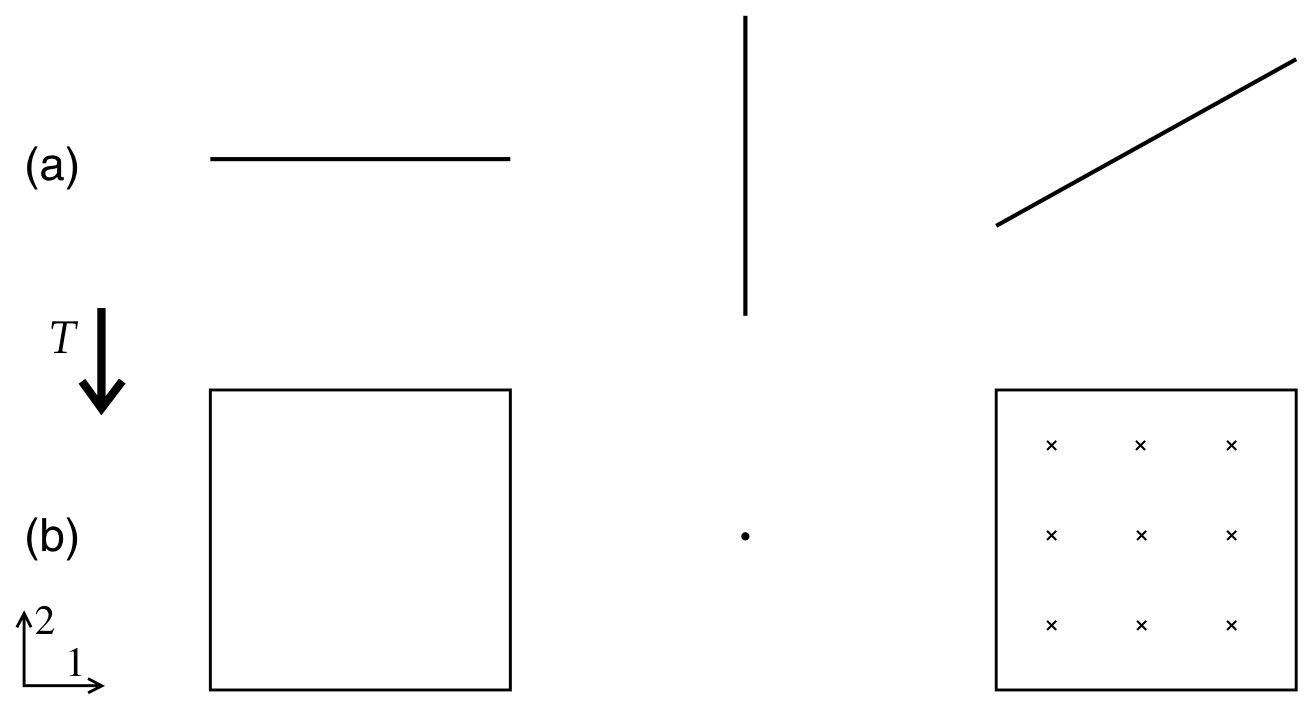
\includegraphics[width=0.75\textwidth]{figure/Fig13.2.jpg}
	\caption{Effect of a T-duality in the 2-direction on D1-branes at various angles in the $(1,2)$ plane: (a) before T-duality; (b) after T-duality. The $\times$s indicate a magnetic field on the D2-brane.}
	\label{fig:13.2}
\end{figure}

The IIB theory also has a 0-form potential $C_{\textit{0}}$, the R--R scalar. This should couple to a `($-1$)-brane.' Indeed, there is a natural interpretation to this: it is defined by Dirichlet boundary conditions in all directions, time as well as space, so its worldsheet is zero-dimensional and the integral \eqref{13.2.7} reduces to the value of $C_{\textit{0}}$ at that point. An object that is localized in time as well as space is an instanton. Instantons in Euclidean path integrals correspond to tunneling events, and these must be present in string theory.

We will verify the R--R couplings of D-branes in the next section; for the remainder of this section we will discuss some of the consequences. The discovery that D-branes carry R--R charges neatly ties together two loose ends. On the one hand, it was argued in section 12.1 that the ordinary string states do not have R--R charges, but now we see that string theory does have a source for every gauge field. This extends the result from chapter 8, that the gauge field from compactification of the antisymmetric tensor couples to winding strings. On the other hand, the existence of so many different kinds of extended object, D$p$-branes for every $p$, might have seemed excessive, but we now see that these are in one-to-one correspondence with the R--R potentials of the respective Type II theories.

The divergence of the Type I theory for groups other than $\mathrm{SO}(32)$ arose from the R--R 10-form field equation. This divergence is unaffected by toroidal compactification and again cancels only for $\mathrm{SO}(32)$. It would have been surprising if toroidal compactification made a consistent theory inconsistent, or the reverse, and it is not hard to verify explicitly that this does not happen. The effect of toroidal compactification is to add worldsheets that wrap around the periodic directions of spacetime. These correspond to exchange of closed strings with winding number, which are massive and so do not have dangerous tadpoles.

The spacetime interpretation of the divergence in the T-dual picture with D-branes is again an inconsistency in the R--R field equations. One can picture field lines emerging from each D-brane, orthogonal to the noncompact dimensions, and these field lines must end somewhere. Further, all D-branes must have the same sign of the charge: the full set of D-branes is still a BPS state, being T-dual to the Type I theory, and the total mass is linear in the total charge for a BPS state. We know that the disk tadpole is canceled by the unoriented cross-cap. In the T-dual spacetime the cross-cap must be localized near one of the orientifold planes, because the string theory in the bulk is oriented. Thus we deduce that the orientifold planes are sinks for R--R charge. If we T-dualize on $k$ dimensions there are $2^k$ orientifold planes but still 16 D-branes, so the charge of an orientifold plane must be $-2^{4-k}$ times that of a D-brane of the same dimension.
\begin{tcolorbox}[breakable]
	\begin{remark}
		\textbf{Conventions.} Charges are counted on the quotient space $T^k/\mathbb Z_2$, where a D-brane and its image count as one object; this is how the text counts ``16 D-branes''. On the covering torus there are 32 branes (16 plus images) and each O-plane appears once.

		Gauss's law on the compact transverse space says the total R--R charge must vanish, since the flux lines have nowhere to go. With D-brane charge $\mu$ and O-plane charge $\mu_{\rm O}$, the $2^k$ fixed planes of $T^k/\mathbb Z_2$ give
		\begin{align*}
			0 = 16\,\mu + 2^k\,\mu_{\rm O} \;\Longrightarrow\; \mu_{\rm O} = -\frac{16}{2^k}\,\mu = -2^{4-k}\,\mu .
		\end{align*}
		The $2^k$ counts the fixed points of $x^m\to-x^m$ on $T^k$: in each circle direction the fixed points are $x^m=0$ and $x^m=\pi R'$, so there are $2$ per direction. For $k=1$ this gives two O8-planes of charge $-8$ each, balancing 16 D8-branes, and for $k=6$ it gives 64 O3-planes of charge $-\frac14$. Counted on the covering space the same statement reads $32\mu+2^k\mu'_{\rm O}=0$ with $\mu'_{\rm O}=-2^{5-k}\mu$. This is the same $-2^{5-k}$ that the text quotes for the D-brane/O-plane force after \eqref{13.3.7}, where it is explained as the flux of the O-plane being squeezed into half the solid angle.
	\end{remark}
\end{tcolorbox}

\subsection*{New Connections Between String Theories}

Starting from the toroidally compactified Type I theory, we can reach either $d = 10$ Type II theory. Simply take an odd or even number of radii to zero, while moving the D-branes and fixed planes off to infinity as the dual spacetime expands. Thus, just as for the two heterotic theories, these should be thought of as limits of a single theory. The theory has many other states as well: we can take the limit while keeping some of the D-branes in fixed positions, so that we obtain the compact theory in a state with D-branes. The simple T-duality leads only to parallel D-branes of equal dimension, but since the D-branes are dynamical we can continuously vary their configurations. We can then reach states with $p$-branes of different dimension as follows. Consider two D1-branes (D-strings) in the IIB theory, from dualizing in eight directions. Let one be along the 1-direction and the other be rotated to lie along the 2-direction. As illustrated in Figure~\ref{fig:13.2}, a further T-duality in the 2-direction reverses Dirichlet and Neumann boundary conditions in this direction and so turns the first D-string into a D2-brane extended in the 1- and 2-directions but the second into a D0-brane. Thus these can coexist in the IIA theory. Of course T-duality leads only to states with 16 D-branes, but we understand now that this is due to the R--R flux conservation in the compact space. In a noncompact space the R--R flux can run to infinity and so any number of D-branes should be allowed.

Thus, starting from the Type I theory we can reach states that look like the Type IIA theory with any collection of even D$p$-branes or the Type IIB theory with any collection of odd D$p$-branes. Of course if we start with an ordinary Type II theory, T-duality will never give us open strings or D-branes, so one might imagine that there is a different Type II theory in which D-branes are not allowed. This seems unlikely, however: everything we know points to the uniqueness of the theory, so we do not have such alternatives. Also, we will see in the next chapter that the inclusion of D-branes leads to a much more elegant and symmetric theory.

In summary, we are now considering a single theory, which has a state that contains no D-branes and looks like the ordinary IIA theory, a second state (T-dual to the first) that contains no D-branes and looks like the ordinary IIB theory, and a third state that contains 16 D9-branes (and an orientifold 9-plane) that looks like the Type I theory. It also contains an infinite number of other states with very general configurations of D-branes.

We can now write down the supersymmetry algebra for this theory:
\begin{subequations} \label{13.2.9}
	\begin{align}
		\{Q_\alpha, Q_\beta\} &= 2(\mathcal{C}\Gamma_\mu)_{\alpha\beta}\bigl(P^\mu + (2\pi\alpha')^{-1}Q_{\mathrm{NS}}^\mu\bigr) \:, \label{13.2.9a} \\
		\{\tilde{Q}_\alpha, \tilde{Q}_\beta\} &= 2(\mathcal{C}\Gamma_\mu)_{\alpha\beta}\bigl(P^\mu - (2\pi\alpha')^{-1}Q_{\mathrm{NS}}^\mu\bigr) \:, \label{13.2.9b} \\
		\{Q_\alpha, \tilde{Q}_\beta\} &= 2\sum_{p}\frac{\tau_p}{p!}Q_{\mathrm{R}}^{\mu_1\dots\mu_p}(\mathcal{C}\beta_{\mu_1}\cdots\beta_{\mu_p})_{\alpha\beta} \:. \label{13.2.9c}
	\end{align}
\end{subequations}
The spacetime supersymmetries $Q_\alpha$ and $\tilde{Q}_\alpha$ act respectively on the left- and right-movers. The anticommutator \eqref{13.2.9b} of two right-moving supersymmetries is the same as the heterotic string anticommutator \eqref{11.6.32}, containing the charge that couples to the NS--NS 2-form. The argument for the appearance of this term is the same as before: the $\tilde{V}_\alpha\tilde{V}_\beta$ OPE contains the right-moving momentum $\bar{\del}X^\mu$, which involves both ordinary momentum and winding number. Similarly, the $V_\alpha V_\beta$ OPE contains the left-moving momentum $\del X^\mu$, so the NS--NS charge appears in the left-moving anticommutator with the opposite sign. We have added a superscript NS to distinguish this charge from the charges $Q_{\mathrm{R}}$ that couple to R--R forms. Also, we have changed conventions so that all charges are now normalized to one per unit worldvolume of the respective extended object, and so the string tension $(2\pi\alpha')^{-1}$ appears explicitly. As discussed in section 11.6, $Q_{\mathrm{NS}}^\mu$ is the charge carried by the fundamental string, meaning the original quantized string. Henceforth we use this term, or F-string, to distinguish it from the D1-brane.

From the argument that D-branes are BPS states, we expect the R--R charges to appear in the algebra as well, and the natural place for an R--R charge to appear is in the anticommutator of a left- and a right-moving supersymmetry. The sum on $p$ runs over even values in the IIA theory and odd values in the IIB theory. By analogy with the NS--NS case we have included the D-brane tensions $\tau_p$, whose values will be obtained in the next section; the factor of $1/p!$ offsets the sum over permutations of indices. To see that the algebra is correct, focus on a state that contains a single static D$p$-brane. The nonzero charge is $Q_{\mathrm{R}}^{\mu_1\dots\mu_p}$, where the indices run over the directions tangent to the D$p$-brane. Note that
\begin{equation}
	\beta_{\mu_1}\cdots\beta_{\mu_p} = \beta_\perp\Gamma^0 \:, \label{13.2.10}
\end{equation}
up to a possible overall sign that can be reabsorbed in the definition of $\tilde{Q}$; $\beta_\perp$ is the same as in equation \eqref{13.2.5}. It then follows that the anticommutator of $Q + \beta_\perp\tilde{Q}$ with any supercharge vanishes in this state, as required by the BPS property. (In equation \eqref{13.2.5} we included primes on the supercharges to indicate that we were working in a T-dual description to the Type I theory with which we began. In writing the algebra \eqref{13.2.9} we are considering an arbitrary state with D-branes, without necessarily obtaining it from T-duality, so there are no primes.)

Incidentally, the central charge \eqref{13.2.9} is still not complete: the magnetic NS--NS charge is missing. This is not carried by D-branes or F-strings. We will discuss this further in the next chapter.

Finally, let us also explain the necessity of D-instantons, localized in time. We could try to use T-duality in the time direction, but it is not clear whether this is meaningful. Rather, consider D0-branes, whose worldlines are one-dimensional, in a space with one compact spatial dimension. For an ordinary quantized particle in a path sum description we would have to include closed paths that wind around the compact direction. Such paths are responsible for Casimir energies and other effects of compactification. Presumably we must do the same for the D0-branes as well. The shortest such winding path is a straight line in the compact spatial direction. This is localized in time and so is essentially an instanton: Casimir energies, in the path sum description, are essentially instanton effects. Further, by a T-duality in the compact dimension we obtain a D-instanton that is localized in all directions. We know from chapter 8 that the D-brane action depends on the closed string coupling as $\mathcal{O}(1/g)$, so the D-instanton amplitude is of order $\me^{-\mathcal{O}(1/g)}$. Thus we have found an example of the enhanced nonperturbative effects that were inferred in section 9.7 from the high order behavior of string perturbation theory.

On the heterotic worldsheet there are no boundary conditions that preserve the worldsheet gauge symmetries, and there is no indication that D-branes exist. Nevertheless, we will see in the next chapter that the D-branes of the Type I/II theory enable us to learn a great deal about the heterotic string as well.


\section{The D-Brane Charge and Action}

There is no force between static BPS objects of like charge. The multi-object state is still supersymmetric and so its energy is determined only by its charge and is independent of the separations. For parallel D$p$-branes, the unbroken supersymmetry \eqref{13.2.5} is the same as for a single D$p$-brane. The vanishing of the force comes about from a cancellation between attraction due to the graviton and dilaton and repulsion due to the R--R tensor. We can calculate these forces explicitly from the usual cylinder vacuum amplitude. The exchange of light NS--NS closed strings was isolated in \eqref{10.8.4}. Modify this expression by removing the factors for the momentum integrations in the Dirichlet directions and introducing a term for the tension of a string stretched over a separation $y^\mu$:
\begin{align}
	\mathcal{A}_{\mathrm{NS-NS}} &\approx \mi V_{p+1}\frac{4\times 16}{8\pi(8\pi^2\alpha')^5}\int_0^\infty \frac{\pi\dif t}{t^2}\,(8\pi^2\alpha' t)^{(9-p)/2}\exp\Bigl(-\frac{t y^2}{2\pi\alpha'}\Bigr) \nonumber \\
	&= \mi V_{p+1} 2\pi(4\pi^2\alpha')^{3-p}G_{9-p}(y) \label{13.3.1}
\end{align}
with $G_d(y) = 2^{-2}\pi^{-d/2}\Gamma(\frac{1}{2}d - 1)y^{2-d}$ the scalar Green's function. The Chan--Paton weight is 2 here, from the two orientations of the open string, and there is no factor of $1/2$ from the orientation projection because the physics is locally oriented.
\begin{tcolorbox}[breakable]
	\begin{remark}
		\textbf{Conventions.} The prefactor $4\times16/[8\pi(8\pi^2\alpha')^5]$ and the measure $\pi\,\dif t/t^2$ are taken from the large-$t$ (closed-string) limit of the cylinder, \eqref{10.8.4}, with the Chan--Paton weight 2 included. $t$ is the open-string modulus, so each open-string state is weighted by $e^{-2\pi tL_0}$ with $L_0=\alpha'(k^2+m^2)+\dots$.

		\textit{Origin of the two modifications.} The momentum integral runs only over the $p+1$ Neumann directions, and a string stretched across the separation $y$ has an extra mass term $L_0\supset\alpha'(y/2\pi\alpha')^2$:
		\begin{align*}
			\int\frac{\dif^{p+1}k}{(2\pi)^{p+1}}\,e^{-2\pi t\alpha'k^2} \eqs{1} (8\pi^2\alpha't)^{-(p+1)/2} = (8\pi^2\alpha't)^{-5}\,(8\pi^2\alpha't)^{(9-p)/2},\\
			e^{-2\pi t\alpha'(y/2\pi\alpha')^2} = \exp\Bigl(-\frac{ty^2}{2\pi\alpha'}\Bigr).
		\end{align*}
		At (1), each Gaussian gives $(2\pi)^{-1}(\pi/2\pi t\alpha')^{1/2}=(8\pi^2\alpha't)^{-1/2}$. The first factor is the ten-dimensional one of \eqref{10.8.4} (together with $V_{10}\to V_{p+1}$), so the rest is the factor $(8\pi^2\alpha't)^{(9-p)/2}$ in \eqref{13.3.1}.

		\textit{The $t$ integral.} With $u=ty^2/2\pi\alpha'$,
		\begin{align*}
			\int_0^\infty \frac{\pi\,\dif t}{t^2}(8\pi^2\alpha't)^{(9-p)/2}e^{-ty^2/2\pi\alpha'}
			&\eqs{2} \pi(8\pi^2\alpha')^{(9-p)/2}\Bigl(\frac{2\pi\alpha'}{y^2}\Bigr)^{(7-p)/2}\Gamma\Bigl(\frac{7-p}{2}\Bigr)\\
			&\eqs{3} \pi(8\pi^2\alpha')^{(9-p)/2}(2\pi\alpha')^{(7-p)/2}\cdot 4\pi^{(9-p)/2}\,G_{9-p}(y) .
		\end{align*}
		At (2), $\int_0^\infty\dif t\,t^{s-1}e^{-at}=a^{-s}\Gamma(s)$ with $s=(7-p)/2$. At (3), $G_{9-p}(y)=\frac14\pi^{-(9-p)/2}\Gamma(\frac{7-p}{2})y^{p-7}$, since $\frac12 d-1=\frac{7-p}{2}$ and $y^{2-d}=y^{p-7}$ for $d=9-p$. Multiplying by the prefactor,
		\begin{align*}
			\frac{\mathcal A_{\rm NS-NS}}{\mi V_{p+1}G_{9-p}(y)} &= \frac{64\,\pi}{8\pi}\cdot4\,(8\pi^2\alpha')^{-(p+1)/2}(2\pi\alpha')^{(7-p)/2}\pi^{(9-p)/2}\\
			&\eqs{4} 2^{7-2p}\pi^{7-2p}{\alpha'}^{3-p} = 2\pi(4\pi^2\alpha')^{3-p} .
		\end{align*}
		At (4) the exponents were collected: for $\alpha'$, $\frac{7-p}{2}-\frac{p+1}{2}=3-p$; for $\pi$, $-(p+1)+\frac{7-p}{2}+\frac{9-p}{2}=7-2p$; for 2, $5-\frac{3(p+1)}{2}+\frac{7-p}{2}=7-2p$. This is the second line of \eqref{13.3.1}.
	\end{remark}
\end{tcolorbox} Due to supersymmetric cancellation in the trace, the R--R exchange amplitude is
\begin{equation}
	\mathcal{A}_{\mathrm{R-R}} = -\mathcal{A}_{\mathrm{NS-NS}} \label{13.3.2}
\end{equation}
and so the total force vanishes as expected.
\begin{tcolorbox}[breakable]
	\begin{remark}
		\textbf{Conventions.} As in section 10.8, the open-string trace over the $p$-$p$ strings on the cylinder is proportional to
		\begin{equation*}
			Z_{00}(\mi t)^4-Z_{01}(\mi t)^4-Z_{10}(\mi t)^4 \ (-Z_{11}^4=0),
		\end{equation*}
		with the terms being, respectively, the NS trace, the NS trace with $(-1)^F$, and the R trace. Under $t\to1/t$ (the closed-string channel), $Z_{00}\to Z_{00}$ and $Z_{01}\leftrightarrow Z_{10}$ up to common factors, by the modular properties \eqref{10.7.14}.

		\textit{Which terms are which exchange.} In the closed channel, a closed-string state propagating between the boundaries is NS--NS if the world-sheet fermions are antiperiodic around the closed-string circle, which is the open-string time direction. That is the case for the open-string traces without the $(-1)^F$ insertion, $Z_{00}^4$ and $Z_{10}^4$; the R--R exchange is the trace with $(-1)^F$ in the NS sector, $Z_{01}^4$. The GSO sign structure gives
		\begin{equation*}
			\mathcal A_{\rm NS-NS}\propto Z_{00}^4-Z_{10}^4,\qquad \mathcal A_{\rm R-R}\propto -Z_{01}^4 ,
		\end{equation*}
		with the same proportionality constant. The abstruse identity \eqref{7.2.41}, $Z_{00}^4-Z_{01}^4-Z_{10}^4=0$, then says $\mathcal A_{\rm NS-NS}=Z_{01}^4\times(\cdots)=-\mathcal A_{\rm R-R}$ at every $t$, not only for the massless exchange, which is \eqref{13.3.2}.
	\end{remark}
\end{tcolorbox}

The field theory calculation \eqref{8.7.25} for the dilaton--graviton potential changes only by the substitution $6 = (D-2)/4 \to 2$, and so is
\begin{equation}
	2\mi\kappa_{10}^2\tau_p^2\,G_{9-p}(y) \:. \label{13.3.3}
\end{equation}
Thus
\begin{equation}
	\tau_p^2 = \frac{\pi}{\kappa_{10}^2}(4\pi^2\alpha')^{3-p} \:. \label{13.3.4}
\end{equation}
This satisfies the same T-duality relation as in the bosonic string.
\begin{tcolorbox}[breakable]
	\begin{remark}
		\textbf{Conventions.} We use the Einstein-frame action of section 8.7 in $D$ dimensions, $\frac{1}{2\kappa^2}\int\dif^Dx\,(-G_{\rm E})^{1/2}\bigl(R-\frac{4}{D-2}\partial_\mu\tilde\Phi\partial^\mu\tilde\Phi\bigr)$ with $\tilde\Phi=\Phi-\Phi_0$. Here $\kappa=\kappa_{10}e^{\Phi_0}$ is the physical gravitational coupling, and the brane action is $-T_p\int e^{-\Phi}(-\det G_{\rm s})^{1/2}$ with $\tau_p=T_pe^{-\Phi_0}$ and $G_{\rm s}=e^{4\tilde\Phi/(D-2)}G_{\rm E}$. For the normalization of an exchange, a canonical scalar $-\frac12(\partial\varphi)^2$ with source coupling $g\varphi$ gives amplitude $\mi g^2G$; in the same normalization the graviton gives $\mi\kappa^2\bigl[T^{\mu\nu}T'_{\mu\nu}-\frac{1}{D-2}TT'\bigr]G$. The Newtonian limit in $D=4$ checks this relative factor: it reproduces $-GMM'/r$ with $8\pi G=\kappa^2$.

		\textit{Graviton.} For a static brane $T^{ab}=-\tau_p\eta^{ab}$ along the $p+1$ worldvolume directions, so
		\begin{align*}
			T^{\mu\nu}T_{\mu\nu}-\frac{T^2}{D-2} = \tau_p^2\Bigl[(p+1)-\frac{(p+1)^2}{D-2}\Bigr] = \tau_p^2\,\frac{(p+1)(D-3-p)}{D-2} .
		\end{align*}
		\textit{Dilaton.} In Einstein frame, $e^{-\Phi}(-\det G_{\rm s})^{1/2}=e^{-\Phi_0}e^{a\tilde\Phi}(-\det G_{\rm E})^{1/2}$ with $a=-1+\frac{2(p+1)}{D-2}=\frac{2p+4-D}{D-2}$, so the brane couples as $-\tau_pa\tilde\Phi$. The canonical field is $\varphi=\tilde\Phi\,[4/(\kappa^2(D-2))]^{1/2}$, so $g^2=\tau_p^2a^2\kappa^2(D-2)/4$. Adding,
		\begin{align*}
			\frac{\mathcal A}{\mi\kappa^2\tau_p^2G} &= \frac{(p+1)(D-3-p)}{D-2} + \frac{(2p+4-D)^2}{4(D-2)}\\
			&\eqs{1} \frac{1}{D-2}\Bigl[q(D-2)-q^2 + q^2 - q(D-2) + \tfrac14(D-2)^2\Bigr] = \frac{D-2}{4} .
		\end{align*}
		At (1), $q=p+1$ was substituted, so $2p+4-D=2q-(D-2)$ and $(p+1)(D-3-p)=q(D-2)-q^2$. The $p$-dependence cancels between graviton and dilaton. For $D=26$ this is the $6$ of \eqref{8.7.25}, and for $D=10$ it is $2$, giving $2\mi\kappa^2\tau_p^2G_{9-p}$, which is \eqref{13.3.3} per unit worldvolume.

		Equating to the NS--NS part of the string amplitude \eqref{13.3.1}, per unit $V_{p+1}$,
		\begin{equation*}
			2\pi(4\pi^2\alpha')^{3-p} = 2\kappa^2\tau_p^2 \;\Longrightarrow\; \tau_p^2=\frac{\pi}{\kappa^2}(4\pi^2\alpha')^{3-p},
			\qquad \frac{\tau_{p-1}^2}{\tau_p^2}=4\pi^2\alpha' ,
		\end{equation*}
		which is \eqref{13.3.4} and the T-duality relation $\tau_{p-1}=2\pi\alpha'^{1/2}\tau_p$ (for $R=\alpha'^{1/2}$) found in the bosonic string.

		\textit{Which $\kappa$.} The graviton and dilaton couple through the physical $\kappa=\kappa_{10}e^{\Phi_0}$, so \eqref{13.3.3}--\eqref{13.3.4} should be read with $\kappa$ rather than $\kappa_{10}$. With $\kappa_{10}$ they would give $\tau_p=\mu_p$, contradicting \eqref{13.3.7}, $\mu_p^2=e^{2\Phi_0}\tau_p^2$, for $\Phi_0\neq0$.
	\end{remark}
\end{tcolorbox}
\noindent For the R--R exchange, the low-energy action is
\begin{equation}
	-\frac{1}{4\kappa_{10}^2}\int \dif^{10}x\,(-G)^{1/2}|F_{p+2}|^2 + \mu_p \int C_{p+1} \:. \label{13.3.5}
\end{equation}
The kinetic term is canonically normalized, so the propagator for any given component (such as the one parallel to the D-brane) is $2\kappa_{10}^2\mi/k^2$, and the field theory amplitude is
\begin{equation}
	-2\kappa_{10}^2\mi\mu_p^2\,G_{9-p}(y) \:. \label{13.3.6}
\end{equation}
Hence
\begin{equation}
	\mu_p^2 = \frac{\pi}{\kappa_{10}^2}(4\pi^2\alpha')^{3-p} = \me^{2\Phi_0}\tau_p^2 = T_p^2 \:. \label{13.3.7}
\end{equation}
\begin{tcolorbox}[breakable]
	\begin{remark}
		\textbf{Conventions.} $|F_{p+2}|^2=\frac{1}{(p+2)!}F_{\mu_1\dots\mu_{p+2}}F^{\mu_1\dots\mu_{p+2}}$ as in section 12.1. The R--R kinetic term in \eqref{13.3.5} has no dilaton factor, so its coupling is $\kappa_{10}$. Exchange amplitudes are normalized as in the previous box: a canonical scalar with source $g\varphi$ gives $\mi g^2G$.

		The brane sources the component $C\equiv C_{01\cdots p}$, and for a static configuration only the transverse gradients $\partial_mC$ matter:
		\begin{align*}
			-\frac{1}{4\kappa_{10}^2}|F_{p+2}|^2 &\eqs{1} -\frac{1}{4\kappa_{10}^2}\sum_m F_{m01\cdots p}F^{m01\cdots p}
			\eqs{2} +\frac{1}{4\kappa_{10}^2}(\partial_mC)^2 ,\\
			C=\sqrt2\,\kappa_{10}\,\varphi \;&\Longrightarrow\; \mu_p\!\int C_{p+1} = \sqrt2\,\kappa_{10}\mu_p\!\int\dif^{p+1}\xi\,\varphi .
		\end{align*}
		At (1), each unordered index set appears $(p+2)!$ times in the sum, cancelling the $1/(p+2)!$, and only sets of the form $\{m,0,1,\dots,p\}$ are nonzero. At (2), raising the index 0 costs $\eta^{00}=-1$. So the static field has the opposite sign of kinetic term to an ordinary scalar, exactly like $A_0$ in electrostatics. Its magnitude is canonical for $\varphi=C/\sqrt2\kappa_{10}$, which is the propagator $2\kappa_{10}^2\mi/k^2$ quoted in the text. The flipped sign makes like charges repel:
		\begin{equation*}
			\mathcal A_{\rm R-R}^{\rm field} = -\mi\bigl(\sqrt2\kappa_{10}\mu_p\bigr)^2G_{9-p} = -2\mi\kappa_{10}^2\mu_p^2\,G_{9-p},
		\end{equation*}
		which is \eqref{13.3.6}. Matching with $\mathcal A_{\rm R-R}=-\mathcal A_{\rm NS-NS}$, \eqref{13.3.2}, and \eqref{13.3.1} per unit volume,
		\begin{align*}
			2\kappa_{10}^2\mu_p^2 = 2\pi(4\pi^2\alpha')^{3-p} \;\Longrightarrow\; \mu_p^2=\frac{\pi}{\kappa_{10}^2}(4\pi^2\alpha')^{3-p} \eqs{3} \frac{\kappa^2}{\kappa_{10}^2}\tau_p^2 \eqs{4} e^{2\Phi_0}\tau_p^2 = T_p^2 .
		\end{align*}
		At (3), \eqref{13.3.4} with the physical $\kappa$ was used. At (4), $\kappa=\kappa_{10}e^{\Phi_0}$, and $T_p=e^{\Phi_0}\tau_p$ is the tension without the $1/g$ of the string-frame action. The cancellation between attraction ($2\kappa^2\tau_p^2$) and repulsion ($2\kappa_{10}^2\mu_p^2$) is therefore the statement $\kappa\tau_p=\kappa_{10}\mu_p$: tension and charge are in the BPS ratio, as the algebra \eqref{bps} requires.
	\end{remark}
\end{tcolorbox}

The reader can carry out a similar calculation of the force between a D-brane and an orientifold plane and show that it has an additional $-2^{5-k}$. We deduced from the cancellation of divergences that the charge of the orientifold plane should have a factor of $-2^{4-k}$; the extra factor of 2 in the force arises because the orientifold geometry squeezes the flux lines into half the solid angle.

The calculation of the interaction confirms our earlier deduction that D-branes carry the R--R charges. It is interesting to see how this is consistent with our earlier discussion of string vertex operators. The R--R vertex operator \eqref{12.1.14} is in the $(-1/2, -1/2)$ picture, which can be used in almost all processes. On the disk, however, the total left- plus right-moving ghost number must be $-2$. With two or more R--R vertex operators, all can be in the $(-1/2, -1/2)$ picture (with PCOs included as well), but a single vertex operator must be in either the $(-3/2, -1/2)$ or the $(-1/2, -3/2)$ picture. The $(-1/2, -1/2)$ vertex operator is essentially $\me^{-\phi}G_0$ times the $(-3/2, -1/2)$ operator, so besides the shift in the ghost number the latter has one less power of momentum and one less $\Gamma$-matrix. The missing factor of momentum turns $F$ into $C$, and the missing $\Gamma$-matrix gives the correct Lorentz representations for the potential rather than the field strength.

\subsection*{Dirac Quantization Condition}

There is an important consistency check on the value of the R--R charge, which generalizes the Dirac quantization condition for magnetic monopole charge. Let us review the Dirac condition, shown in Figure~\ref{fig:13.3}. Consider a magnetic charge $\mu_{\mathrm{m}}$ at the origin. The integrated flux is
\begin{equation}
	\int_{S^2} F_{\textit{2}} = \mu_{\mathrm{m}} \:. \label{13.3.8}
\end{equation}
Because the integral over a closed surface is nonzero, we cannot write $F_{\textit{2}} = \dif A_{\textit{1}}$ for any globally well-defined vector potential. However, we can write $F_{\textit{2}} = \dif A_{\textit{1}}$ except along a Dirac string ending on the monopole. Now consider an electric charge $\mu_{\mathrm{e}}$ moving in this field. Its coupling to the field produces a phase
\begin{equation}
	\exp\Bigl(\mi\mu_{\mathrm{e}}\int_P A_{\textit{1}}\Bigr) = \exp\Bigl(\mi\mu_{\mathrm{e}}\int_D F_{\textit{2}}\Bigr) \label{13.3.9}
\end{equation}
when the particle moves on a closed path $P$. The surface $D$ spans $P$ and does not intersect the Dirac string. Now consider the limit as the path is contracted to a small circle around the Dirac string. The phase becomes
\begin{equation}
	\exp\Bigl(\mi\mu_{\mathrm{e}}\int_{S^2} F_{\textit{2}}\Bigr) = \exp(\mi\mu_{\mathrm{e}}\mu_{\mathrm{m}}) \:. \label{13.3.10}
\end{equation}
The Dirac string must be invisible, so this phase must be 1. Equivalently, this is the condition that the phase \eqref{13.3.9} is unchanged if we replace $D$ with a surface $D'$ that passes on the other side of the monopole, so $D - D' = S^2$. The condition is
\begin{equation}
	\mu_{\mathrm{e}}\mu_{\mathrm{m}} = 2\pi n \label{13.3.11}
\end{equation}
with $n$ an integer.

\begin{figure}[htbp]
	\centering
	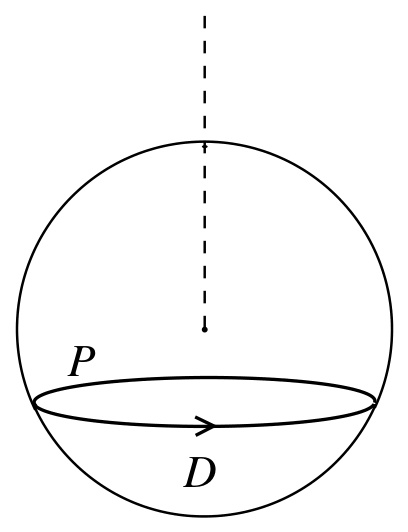
\includegraphics[width=0.35\textwidth]{figure/Fig13.3.jpg}
	\caption{Sphere surrounding monopole, with a Dirac string running upward. The particle path $P$ is bounded by the lower cap $D$.}
	\label{fig:13.3}
\end{figure}

The Dirac condition generalizes directly to extended objects and their charges. Let us think about $F_{p+2}$ as the field strength, so that the $p$-brane is an electric source and the $(6-p)$-brane a magnetic source. In nine dimensions a $(6-p)$-dimensional object is surrounded by a $(p+2)$-sphere, so by analogy to the magnetic flux \eqref{13.3.8},
\begin{equation}
	\int_{S^{p+2}} F_{p+2} = \frac{2\kappa_{10}^2}{\mu_{6-p}} \:. \label{13.3.12}
\end{equation}
One can then repeat the same argument. For example, let the $p$-brane be extended in the directions $4 \le \mu \le p+3$ and the $(6-p)$-brane in the directions $p+4 \le \mu \le 9$. The system essentially reduces to the three-dimensional situation of Figure~\ref{fig:13.3} in the directions $\mu = 1, 2, 3$, and the charges must satisfy
\begin{equation}
	2\kappa_{10}^2\mu_p\mu_{6-p} = 2\pi n \:. \label{13.3.13}
\end{equation}
Remarkably, the charges \eqref{13.3.7}, arrived at in an entirely different way, satisfy this relation with the minimum quantum $n = 1$.
\begin{tcolorbox}[breakable]
	\begin{remark}
		\textbf{Conventions.} The $(6-p)$-brane is an electric source for $C_{7-p}$, with action $-\frac{1}{4\kappa_{10}^2}\int F_{8-p}\wedge*F_{8-p}+\mu_{6-p}\int C_{7-p}$. Here $\int\dif^{10}x\,(-G)^{1/2}|F|^2=\int F\wedge*F$, and $F_{p+2}=\pm*F_{8-p}$ describes the same field. Overall orientation signs are dropped; only magnitudes enter the Dirac condition.

		\textit{Flux of the magnetic source.} Varying $C_{7-p}$,
		\begin{align*}
			0=\delta S &= -\frac{1}{2\kappa_{10}^2}\int \dif\,\delta C_{7-p}\wedge*F_{8-p} + \mu_{6-p}\int_{\mathcal W}\delta C_{7-p}\\
			&\eqs{1} \pm\frac{1}{2\kappa_{10}^2}\int\delta C_{7-p}\wedge\dif*F_{8-p} + \mu_{6-p}\int\delta C_{7-p}\wedge\delta_{\mathcal W} ,\\
			\int_{S^{p+2}}F_{p+2} &\eqs{2} \pm\int_{S^{p+2}}*F_{8-p} \eqs{3} \pm\int_{B^{p+3}}\dif*F_{8-p}\\
			&= 2\kappa_{10}^2\,\mu_{6-p} .
		\end{align*}
		At (1), integration by parts, with $\delta_{\mathcal W}$ the $(p+3)$-form delta function transverse to the worldvolume. At (2), $F_{p+2}=\pm*F_{8-p}$. At (3), Stokes's theorem on the ball whose boundary is the $(p+2)$-sphere around the $(6-p)$-brane, and the field equation $\dif*F_{8-p}=\pm2\kappa_{10}^2\mu_{6-p}\delta_{\mathcal W}$. So the flux is $2\kappa_{10}^2\mu_{6-p}$, not $2\kappa_{10}^2/\mu_{6-p}$ as printed in \eqref{13.3.12}. With this flux, the Dirac argument \eqref{13.3.9}--\eqref{13.3.11} with $\mu_{\rm e}=\mu_p$ and $\mu_{\rm m}=2\kappa_{10}^2\mu_{6-p}$ gives \eqref{13.3.13} as printed. The printed \eqref{13.3.12} would instead give $2\kappa_{10}^2\mu_p/\mu_{6-p}=2\pi n$, which is not symmetric between the two branes.

		\textit{Check with \eqref{13.3.7}.}
		\begin{align*}
			\mu_p^2\mu_{6-p}^2 = \frac{\pi^2}{\kappa_{10}^4}(4\pi^2\alpha')^{3-p}(4\pi^2\alpha')^{3-(6-p)} \eqs{4} \frac{\pi^2}{\kappa_{10}^4}
			\;\Longrightarrow\; 2\kappa_{10}^2\mu_p\mu_{6-p} = 2\pi .
		\end{align*}
		At (4), the exponents $3-p$ and $p-3$ cancel, so $\alpha'$ drops out. The minimal quantum $n=1$ is saturated for every $p$.
	\end{remark}
\end{tcolorbox}

\subsection*{D-Brane Actions}

The coupling of a D-brane to NS--NS closed string fields is the same Dirac--Born--Infeld action as in the bosonic string:
\begin{equation}
	S_{\mathrm{D}p} = -\mu_p\int \dif^{p+1}\xi\,\operatorname{Tr}\Bigl(\me^{-\Phi}\bigl[-\det(G_{ab} + B_{ab} + 2\pi\alpha' F_{ab})\bigr]^{1/2}\Bigr) \:, \label{13.3.14}
\end{equation}
where $G_{ab}$ and $B_{ab}$ are the components of the spacetime NS--NS fields parallel to the brane and $F_{ab}$ is the gauge field living on the brane. The argument leading to this form is exactly as in the bosonic case, section 8.7. Recall that for $n$ D-branes at small separation, where the strings stretched between them are light enough to be included in the low energy action, the collective coordinates $X^\mu(\xi)$, gauge fields $A_a(\xi)$, and their fermionic partners $\lambda(\xi)$ all become $n \times n$ matrices. The trace in the action is in this $n \times n$ space. In addition there is a term
\begin{equation}
	\mathcal{O}([X^m, X^n]^2) \label{13.3.15}
\end{equation}
in the potential. As discussed in chapter 8, the effect of this potential is that in the flat directions the collective coordinates become diagonal. They can then be interpreted as $n$ ordinary collective coordinates for $n$ objects. At small separation the full matrix dynamics is crucial, as we will see.

The coupling to the R--R background also includes corrections involving the gauge field on the brane. Like the Born--Infeld action, these can be deduced via T-duality. Consider, as an example, a 1-brane in the $(1,2)$ plane. The action is
\begin{equation}
	\int C_{\textit{2}} = \int \dif x^0(\dif x^1 C_{01} + \dif x^2 C_{02}) = \int \dif x^0\dif x^1\bigl(C_{01} + \del_1 X^2 C_{02}\bigr) \:. \label{13.3.16}
\end{equation}
Under a T-duality in the 2-direction this becomes:
\begin{equation}
	\int \dif x^0\dif x^1\bigl(C_{012} + 2\pi\alpha' F_{12}C_0\bigr) \:. \label{13.3.17}
\end{equation}
We have used the T-transformation of the $C$ fields, \eqref{13.1.5}. A D-brane at an angle is T-dual to one with a magnetic field, as in Figure~\ref{fig:13.2}. We are not keeping track of the normalization but one could, with the result $\mu_p = \mu_{p-1}/(2\pi{\alpha'}^{1/2})$ in agreement with the explicit calculation. The generalization of \eqref{13.3.17} to an arbitrary configuration, and to multiple D-branes, gives the Chern--Simons-like result
\begin{equation}
	\mi\mu_p\int_{\mathcal{W}_{p+1}}\operatorname{Tr}\Bigl[\exp\bigl(2\pi\alpha' F_{\textit{2}} + B_{\textit{2}}\bigr)\wedge \sum_{q}C_q\Bigr] \:. \label{13.3.18}
\end{equation}
The expansion of the integrand \eqref{13.3.18} involves forms of various rank; the integral picks out precisely the terms that are proportional to the volume form of the $p$-brane worldvolume. There are similar couplings with the spacetime curvature in addition to the field strength; these can be obtained from a string calculation:
\[
S_{\mathrm{WZ}} = \mi\mu_p\int_{\mathcal{W}_{p+1}}\operatorname{Tr}\Bigl[\exp\bigl(2\pi\alpha' F_{\textit{2}} + B_{\textit{2}}\bigr)\wedge \sum_{q}C_q\Bigr]\wedge \sqrt{\hat{A}(\mathcal{R})} \:.
\]
\begin{tcolorbox}[breakable]
	\begin{remark}
		\textbf{Conventions.} Static gauge $\xi^a=x^a$ is used, and the transverse position of the D1-brane is $X^2(x^0,x^1)$. The T-duality dictionary of chapter 8 is $X^m=2\pi\alpha'A_m$ for a dualized direction $m$, with fields independent of $x^2$. Signs from \eqref{13.1.5} (``up to signs'') are dropped, as in the text.

		\textit{From \eqref{13.3.16} to \eqref{13.3.17}.} The pullback of $C_2$ to the tilted string is
		\begin{align*}
			\int C_{\textit{2}} &= \int \dif x^0\wedge\bigl(\dif x^1C_{01}+\dif x^2C_{02}\bigr) \eqs{1} \int\dif x^0\dif x^1\bigl(C_{01}+\partial_1X^2\,C_{02}\bigr)\\
			&\eqs{2} \int\dif x^0\dif x^1\bigl(C_{012}+2\pi\alpha'\partial_1A_2\,C_0\bigr) \eqs{3} \int\dif x^0\dif x^1\bigl(C_{012}+2\pi\alpha'F_{12}\,C_0\bigr).
		\end{align*}
		At (1), $\dif x^2=\partial_1X^2\,\dif x^1+\partial_0X^2\,\dif x^0$ on the worldsheet, and the $\dif x^0$ term drops against $\dif x^0$. At (2), \eqref{13.1.5}: $C_{01}$ gains the index 2, $C_{02}$ loses it, and $X^2\to2\pi\alpha'A_2$. At (3), $F_{12}=\partial_1A_2-\partial_2A_1=\partial_1A_2$ because nothing depends on $x^2$. The worldvolume is now the D2-brane along $x^0,x^1,x^2$, and $\int\dif x^2$ gives the dual circle's length, which is where the normalization $\mu_2=\mu_1/(2\pi\alpha'^{1/2})$ enters. From \eqref{13.3.7} in general, $\mu_p/\mu_{p-1}=(4\pi^2\alpha')^{-1/2}=1/(2\pi\alpha'^{1/2})$.

		\textit{Expansion of \eqref{13.3.18}.} For one brane and $B=0$, the $(p+1)$-form part of the integrand is
		\begin{align*}
			\Bigl[e^{2\pi\alpha'F}\wedge\sum_qC_q\Bigr]_{p+1} = C_{p+1} + 2\pi\alpha'F\wedge C_{p-1} + \frac{(2\pi\alpha')^2}{2}F\wedge F\wedge C_{p-3} + \cdots .
		\end{align*}
		For $p=2$ the first two terms are $C_{012}\,\dif x^0\dif x^1\dif x^2$ and $2\pi\alpha'F_{12}C_0\,\dif x^1\wedge\dif x^2\wedge\dif x^0$, reproducing \eqref{13.3.17} up to orientation. The term $\frac12(2\pi\alpha')^2F\wedge F\wedge C_{p-3}$ says that an instanton ($\int F\wedge F\neq0$) on a D$p$-brane carries D$(p-4)$ charge; this is used for the D0--D4 system in section 13.6. The combination $2\pi\alpha'F+B$ is fixed because it is the invariant combination under the NS--NS gauge transformation $\delta B=\dif\zeta$, $\delta A=-\zeta/2\pi\alpha'$.
	\end{remark}
\end{tcolorbox}

Thus far we have given only the action for the bosonic fields on the brane. For the leading fluctuations around a flat D-brane in flat spacetime the fermionic action is of the usual Dirac form:
\begin{equation}
	-\mi\int \dif^{p+1}\xi\,\operatorname{Tr}(\bar{\lambda}\Gamma^a D_a\lambda) \:. \label{13.3.19}
\end{equation}
The full nonlinear supersymmetric form is left to the references.

\subsection*{Coupling Constants}

The ratio of the F-string tension to the D-string tension is
\begin{equation}
	\frac{\tau_{\mathrm{F}1}}{\tau_{\mathrm{D}1}} = \frac{1/(2\pi\alpha')}{\kappa/(4\pi^{5/2}\alpha')} = \frac{\kappa}{8\pi^{7/2}{\alpha'}^2} \:. \label{13.3.20}
\end{equation}
Up to now there has been no natural convention for defining the additive normalization of the dilaton field or the multiplicative normalization of the closed string coupling $g = \me^{\Phi}$. The dimensionless ratio \eqref{13.3.20} is proportional to the closed string coupling, and it turns out to be very convenient to take it as the definition of the coupling:
\begin{equation}
	g = \frac{\tau_{\mathrm{F}1}}{\tau_{\mathrm{D}1}} \:. \label{13.3.21}
\end{equation}
Then the gravitational coupling is
\begin{equation}
	\kappa^2 = \frac{1}{2}(2\pi)^7 g^2 {\alpha'}^4 \label{13.3.22}
\end{equation}
and the D-brane tension is
\begin{equation}
	\tau_p = \frac{1}{g(2\pi)^p{\alpha'}^{(p+1)/2}} = (2\kappa^2)^{-1/2}(2\pi)^{(7-2p)/2}{\alpha'}^{(3-p)/2} \:. \label{13.3.23}
\end{equation}
Also, the constant appearing in the low energy actions of section 12.1 is
\begin{equation}
	\kappa_{10}^2 = \frac{1}{2}(2\pi)^7{\alpha'}^4 \:; \label{13.3.24}
\end{equation}
this differs from the physically measured $\kappa$ because the latter depends on the dilaton background.

Expanding the action \eqref{13.3.14} gives the coupling of the Yang--Mills theory on the D$p$-brane:
\begin{equation}
	g_{\mathrm{D}p}^2 = \frac{1}{(2\pi\alpha')^2\tau_p} = (2\pi)^{p-2}g{\alpha'}^{(p-3)/2} \:. \label{13.3.25}
\end{equation}
Notice that for $p = 3$ this coupling is dimensionless, as expected in a $(3 + 1)$-dimensional gauge theory. For $p < 3$ the coupling has units of length to a negative power, and for $p > 3$ length to a positive power.
\begin{tcolorbox}[breakable]
	\begin{remark}
		\textbf{Conventions.} In this subsection $\kappa=\kappa_{10}e^{\Phi_0}$ is the physical coupling and $\tau_p$ the physical tension of \eqref{13.3.4}, $\tau_p^2=\pi(4\pi^2\alpha')^{3-p}/\kappa^2$. The Yang--Mills normalization is $-\frac{1}{4g^2}\int F_{ab}F^{ab}$ for a $\mathrm U(1)$ factor (then $\operatorname{Tr}_{\rm f}$ for $\mathrm U(n)$, \eqref{13.3.26}).

		\textit{The D-string tension and \eqref{13.3.20}.}
		\begin{align*}
			\tau_{\rm D1}^2 \eqs{1} \frac{\pi}{\kappa^2}(4\pi^2\alpha')^2 = \frac{16\pi^5{\alpha'}^2}{\kappa^2}
			\;\Longrightarrow\; \tau_{\rm D1}=\frac{4\pi^{5/2}\alpha'}{\kappa},\qquad
			\frac{\tau_{\rm F1}}{\tau_{\rm D1}} = \frac{1/(2\pi\alpha')}{4\pi^{5/2}\alpha'/\kappa} = \frac{\kappa}{8\pi^{7/2}{\alpha'}^2} .
		\end{align*}
		At (1), \eqref{13.3.4} was used with $p=1$. The final value in \eqref{13.3.20} is correct, but its middle expression has $\tau_{\rm D1}$ inverted: the denominator should read $4\pi^{5/2}\alpha'/\kappa$, not $\kappa/(4\pi^{5/2}\alpha')$.

		\textit{\eqref{13.3.22}--\eqref{13.3.24}.} With $g=\kappa/(8\pi^{7/2}\alpha'^2)$,
		\begin{align*}
			\kappa^2 &= 64\pi^7g^2{\alpha'}^4 \eqs{2} \tfrac12(2\pi)^7g^2{\alpha'}^4, \qquad \kappa=2^{-1/2}(2\pi)^{7/2}g\,{\alpha'}^2,\\
			\tau_p &= \frac{\pi^{1/2}}{\kappa}(2\pi)^{3-p}{\alpha'}^{(3-p)/2} \eqs{3} \frac{(2\pi)^{1/2}(2\pi)^{3-p}{\alpha'}^{(3-p)/2}}{(2\pi)^{7/2}g{\alpha'}^2} = \frac{1}{g(2\pi)^p{\alpha'}^{(p+1)/2}} ,\\
			\tau_p &\eqs{4} (2\kappa^2)^{-1/2}(2\pi)^{1/2}(2\pi)^{3-p}{\alpha'}^{(3-p)/2} = (2\kappa^2)^{-1/2}(2\pi)^{(7-2p)/2}{\alpha'}^{(3-p)/2},\\
			\kappa_{10}^2 &= \frac{\kappa^2}{g^2} = \tfrac12(2\pi)^7{\alpha'}^4 .
		\end{align*}
		At (2), $(2\pi)^7=128\pi^7$. At (3), $\pi^{1/2}\cdot2^{1/2}=(2\pi)^{1/2}$ and $\kappa$ was substituted. At (4), $\pi^{1/2}/\kappa=(2\pi)^{1/2}/(2\kappa^2)^{1/2}$. The last relation uses $\kappa=\kappa_{10}e^{\Phi_0}$ and $g=e^{\Phi_0}$ in the normalization \eqref{13.3.21}.

		\textit{\eqref{13.3.25}.} Expand \eqref{13.3.14} in flat space with $B=0$, constant dilaton, and one brane. With $M^a{}_b=2\pi\alpha'F^a{}_b$,
		\begin{align*}
			\bigl[-\det(\eta_{ab}+2\pi\alpha'F_{ab})\bigr]^{1/2} &= \det\,^{1/2}(1 + M) \\ &\eqs{5} 1+\tfrac12\operatorname{tr}M-\tfrac14\operatorname{tr}M^2+\tfrac18(\operatorname{tr}M)^2+\cdots\\
			&\eqs{6} 1+\tfrac14(2\pi\alpha')^2F_{ab}F^{ab}+\cdots ,\\
			S_{\rm D\it p} &\supset -\tau_p\frac{(2\pi\alpha')^2}{4}\int\dif^{p+1}\xi\,F_{ab}F^{ab}\\ &\equiv -\frac{1}{4g_{{\rm D}p}^2}\int\dif^{p+1}\xi\,F_{ab}F^{ab}\\
			&\;\Longrightarrow\; g_{{\rm D}p}^2=\frac{1}{(2\pi\alpha')^2\tau_p} .
		\end{align*}
		At (5), $\det\,^{1/2}(1 + M)=\exp\frac12\operatorname{tr}\ln(1+M)$ was expanded to second order. At (6), $\operatorname{tr}M=2\pi\alpha'F^a{}_a=0$ by antisymmetry, and $\operatorname{tr}M^2=(2\pi\alpha')^2F^a{}_bF^b{}_a=-(2\pi\alpha')^2F_{ab}F^{ab}$. The prefactor $\mu_pe^{-\Phi_0}$ is $\tau_p$. Inserting $\tau_p$ from above,
		\begin{equation*}
			g_{{\rm D}p}^2 = \frac{g(2\pi)^p{\alpha'}^{(p+1)/2}}{4\pi^2{\alpha'}^2} = (2\pi)^{p-2}g\,{\alpha'}^{(p-3)/2},
		\end{equation*}
		which is \eqref{13.3.25}. Its mass dimension is $3-p$, since $[\alpha']=-2$ and $g$ is dimensionless.
	\end{remark}
\end{tcolorbox}

We now wish to obtain the relation among $\kappa$, $g_{\mathrm{YM}}$, and $\alpha'$ in the Type I theory. We cannot quite identify $g_{\mathrm{D}p}$ for $p = 9$ with $g_{\mathrm{YM}}$, because the former has been obtained in a locally oriented theory and there are some additional factors of 2 in the Type I case. Rather than repeat the string calculation we will make a more roundabout but possibly instructive argument using T-duality.

First, we should note that the coupling \eqref{13.3.25} is for the $\mathrm{U}(n)$ gauge theory of coincident branes in the oriented theory: it appears in the form
\begin{equation}
	\frac{1}{4g_{\mathrm{D}p}^2}\operatorname{Tr}_{\mathrm{f}} \:, \label{13.3.26}
\end{equation}
where the trace is in the $n \times n$ fundamental representation. Now let us consider moving the branes to an orientifold plane so that the gauge symmetry is enlarged to $\mathrm{SO}(2n)$. An $\mathrm{SU}(n)$ generator $t$ is embedded in $\mathrm{SO}(2n)$ as
\begin{equation}
	\tilde{t} = \begin{pmatrix} t & 0 \\ 0 & -t^{\mathrm{T}} \end{pmatrix} \:, \label{13.3.27}
\end{equation}
because the orientation projection reverses the order of the Chan--Paton factors and the sign of the gauge field. Comparing the low energy actions gives
\begin{equation}
	\frac{1}{4g_{\mathrm{D}p}^2}\operatorname{Tr}_{\mathrm{f}}(t^2) = \frac{1}{4g_{\mathrm{D}p,\mathrm{SO}(2n)}^2}\operatorname{Tr}_{\mathrm{v}}(\tilde{t}^2) \label{13.3.28}
\end{equation}
and so $g_{\mathrm{D}p,\mathrm{SO}(2n)}^2 = 2g_{\mathrm{D}p}^2$.

Now consider the Type I theory compactified on a $k$-torus with all radii equal to $R$. The couplings in the lower-dimensional $\mathrm{SO}(32)$ theory are related to those in the Type I theory by
\begin{equation}
	\kappa_{10-k}^2 = (2\pi R)^{-k}\kappa^2 \quad (\text{Type I}) \:, \quad g_{10-k,\mathrm{YM}}^2 = (2\pi R)^{-k}g_{\mathrm{YM}}^2 \quad (\text{Type I}) \:. \label{13.3.29}
\end{equation}
In the T-dual picture, the bulk theory is of Type II and the gauge fields live on a D$(9-k)$-brane, and
\begin{equation}
	\kappa_{10-k}^2 = 2(2\pi R')^{-k}\kappa^2 \:, \quad g_{10-k,\mathrm{YM}}^2 = g_{\mathrm{D}(9-k),\mathrm{SO}(32)}^2 \:. \label{13.3.30}
\end{equation}
The dimensional reduction for $\kappa_{10-k}^2$ has an extra factor of 2 because the compact space is an orientifold, its volume halved. The gauge coupling is independent of the volume because the fields are localized on the D-brane. Combining these results with the relations \eqref{13.3.22} and \eqref{13.3.25} gives, independent of $k$, the Type I relation:
\begin{equation}
	\frac{g_{\mathrm{YM}}^2}{\kappa} = 2(2\pi)^{7/2}\alpha' \quad (\text{Type I}) \:. \label{13.3.31}
\end{equation}
\begin{tcolorbox}[breakable]
	\begin{remark}
		\textbf{Conventions.} $\kappa_{\rm I}$ and $g_{\rm YM}$ are the ten-dimensional Type I couplings. $\kappa_{\rm II}$ and $g_{\rm II}$ are those of the T-dual Type II bulk, related by \eqref{13.3.22}, and the dual radius is $R'=\alpha'/R$.

		\textit{\eqref{13.3.28}.} For the embedding \eqref{13.3.27},
		\begin{equation*}
			\operatorname{Tr}_{\rm v}(\tilde t^2)=\operatorname{Tr}_{\rm f}(t^2)+\operatorname{Tr}_{\rm f}\bigl((t^{\mathrm T})^2\bigr)=2\operatorname{Tr}_{\rm f}(t^2)
			\;\Longrightarrow\; \frac{1}{4g_{{\rm D}p}^2}=\frac{2}{4g^2_{{\rm D}p,\mathrm{SO}(2n)}},\quad g^2_{{\rm D}p,\mathrm{SO}(2n)}=2g_{{\rm D}p}^2 .
		\end{equation*}

		\textit{The ratio $g^2_{10-k}/\kappa_{10-k}$ computed two ways.} From \eqref{13.3.29},
		\begin{equation*}
			\frac{g^2_{10-k,\rm YM}}{\kappa_{10-k}} = \frac{g_{\rm YM}^2}{\kappa_{\rm I}}(2\pi R)^{-k/2} .
		\end{equation*}
		From \eqref{13.3.30}, with $g^2_{{\rm D}(9-k),\mathrm{SO}(32)}=2g^2_{{\rm D}(9-k)}=2(2\pi)^{7-k}g_{\rm II}{\alpha'}^{(6-k)/2}$ from \eqref{13.3.25} with $p=9-k$,
		\begin{align*}
			\frac{g^2_{10-k,\rm YM}}{\kappa_{10-k}} &= \frac{2(2\pi)^{7-k}g_{\rm II}{\alpha'}^{(6-k)/2}}{\sqrt2\,\kappa_{\rm II}(2\pi R')^{-k/2}}
			\eqs{1} \frac{2(2\pi)^{7-k}{\alpha'}^{(6-k)/2}(2\pi R')^{k/2}}{(2\pi)^{7/2}{\alpha'}^2}\\
			&= 2(2\pi)^{7/2-k}{\alpha'}^{1-k/2}(2\pi R')^{k/2} .
		\end{align*}
		At (1), $\sqrt2\,\kappa_{\rm II}/g_{\rm II}=(2\pi)^{7/2}{\alpha'}^2$ by \eqref{13.3.22}. Equating the two,
		\begin{align*}
			\frac{g_{\rm YM}^2}{\kappa_{\rm I}} = 2(2\pi)^{7/2-k}{\alpha'}^{1-k/2}\bigl(4\pi^2RR'\bigr)^{k/2} \eqs{2} 2(2\pi)^{7/2-k}{\alpha'}^{1-k/2}(2\pi)^k{\alpha'}^{k/2} = 2(2\pi)^{7/2}\alpha' .
		\end{align*}
		At (2), $RR'=\alpha'$. All dependence on $k$ and on the radii cancels, as it must for a ten-dimensional relation, giving \eqref{13.3.31}.
	\end{remark}
\end{tcolorbox}

As one final remark, the Born--Infeld form for the gauge action applies by T-duality to the Type I theory:
\begin{equation}
	S = -\frac{1}{(2\pi\alpha')^2 g_{\mathrm{YM}}^2}\int \dif^{10}x\,\operatorname{Tr}\Bigl(\bigl[-\det(\eta_{\mu\nu} + 2\pi\alpha' F_{\mu\nu})\bigr]^{1/2}\Bigr) \:, \label{13.3.32}
\end{equation}
whose normalization is fixed by the quadratic term in $F$. In the previous chapter we obtained the tree-level string correction \eqref{12.4.28} to the Type I effective action. If the gauge field lies in an Abelian subgroup, the tensor structure simplifies to
\begin{equation}
	\frac{(2\pi\alpha')^2}{32g_{\mathrm{YM}}^2}\operatorname{Tr}_{\mathrm{v}}\bigl(4F_{\mu\nu}F^{\nu\sigma}F_{\sigma\rho}F^{\rho\mu} - F_{\mu\nu}F^{\nu\mu}F_{\sigma\rho}F^{\rho\sigma}\bigr) \:. \label{13.3.33}
\end{equation}
This is indeed the quartic term in the expansion of the Born--Infeld action, as one finds by using
\begin{equation}
	\det\,^{1/2}(1 + M) = \exp\biggl(\frac{1}{2}\operatorname{tr}\Bigl(M - \frac{1}{2}M^2 + \frac{1}{3}M^3 - \frac{1}{4}M^4 + \dots\Bigr)\biggr) \label{13.3.34}
\end{equation}
with $M^\mu{}_\nu = 2\pi\alpha' F^\mu{}_\sigma \eta^{\sigma\nu}$. The trace here is on the Lorentz indices, and $\operatorname{tr}(x^{2k+1}) = 0$ for antisymmetric $x$. Note that only when the gauge field can be diagonalized can we give a geometric interpretation to the T-dual configuration and so derive the Born--Infeld form.
\begin{tcolorbox}[breakable]
	\begin{remark}
		\textbf{Conventions.} The gauge field lies in an Abelian subgroup, so the $F$'s commute and the gauge trace $\operatorname{Tr}_{\rm v}$ can be taken outside, and $\operatorname{Tr}$ in \eqref{13.3.32} is $\operatorname{Tr}_{\rm v}$. $\operatorname{tr}$ is the Lorentz trace.

		\textit{Proof of \eqref{13.3.34}.} $\det(1+M)=\exp\operatorname{tr}\ln(1+M)$ and $\ln(1+M)=M-\frac12M^2+\frac13M^3-\frac14M^4+\cdots$. Taking the square root halves the exponent.

		\textit{The expansion.} Since $M_{\mu\nu}=2\pi\alpha'F_{\mu\nu}$ is antisymmetric, $\operatorname{tr}M=\operatorname{tr}M^3=0$ and
		\begin{align*}
			\det\,^{1/2}(1 + M) &\eqs{1} \exp\Bigl(-\tfrac14\operatorname{tr}M^2-\tfrac18\operatorname{tr}M^4+\cdots\Bigr)\\
			&\eqs{2} 1-\tfrac14\operatorname{tr}M^2-\tfrac18\operatorname{tr}M^4+\tfrac1{32}\bigl(\operatorname{tr}M^2\bigr)^2+\cdots ,\\
			\operatorname{tr}M^2 &= (2\pi\alpha')^2F_{\mu\nu}F^{\nu\mu},\\ \operatorname{tr}M^4&=(2\pi\alpha')^4F_{\mu\nu}F^{\nu\sigma}F_{\sigma\rho}F^{\rho\mu} .
		\end{align*}
		At (1) the odd traces were dropped. At (2) the exponential was expanded to fourth order in $F$, where $\frac12\bigl(\frac14\operatorname{tr}M^2\bigr)^2=\frac1{32}(\operatorname{tr}M^2)^2$. Inserting into \eqref{13.3.32},
		\begin{align*}
			S &\supset -\frac{1}{(2\pi\alpha')^2g_{\rm YM}^2}\int\dif^{10}x\operatorname{Tr}_{\rm v}\Bigl[-\tfrac14(2\pi\alpha')^2F_{\mu\nu}F^{\nu\mu}\Bigr]
			= -\frac{1}{4g_{\rm YM}^2}\int\dif^{10}x\operatorname{Tr}_{\rm v}F_{\mu\nu}F^{\mu\nu},\\
			S &\supset -\frac{(2\pi\alpha')^4}{(2\pi\alpha')^2g_{\rm YM}^2}\int\dif^{10}x\operatorname{Tr}_{\rm v}\Bigl[-\tfrac18F_{\mu\nu}F^{\nu\sigma}F_{\sigma\rho}F^{\rho\mu}+\tfrac1{32}\bigl(F_{\mu\nu}F^{\nu\mu}\bigr)^2\Bigr] \\
			&= \frac{(2\pi\alpha')^2}{32g_{\rm YM}^2}\int\dif^{10}x\operatorname{Tr}_{\rm v}\bigl(4F_{\mu\nu}F^{\nu\sigma}F_{\sigma\rho}F^{\rho\mu}-F_{\mu\nu}F^{\nu\mu}F_{\sigma\rho}F^{\rho\sigma}\bigr) .
		\end{align*}
		The first line is canonical Yang--Mills, which fixes the prefactor of \eqref{13.3.32}. The last line is exactly \eqref{13.3.33}, the quartic term found from the four-point string amplitude.
	\end{remark}
\end{tcolorbox}


\section{D-Brane Interactions: Statics}

In this section and the following two we study the interaction between two D-branes. In this section we will calculate the static force and study the conditions for supersymmetry to be unbroken. In the next section we will consider moving D-branes. In section 13.6 we will study bound states of D-branes.

\subsection*{Branes with Mixed Boundary Conditions}

Consider two flat D-branes, a D$p$-brane and a D$p'$-brane, and open strings stretched between them (the $p$-$p'$ strings). In each spatial direction, the open string satisfies Neumann (N) or Dirichlet (D) boundary conditions at each end. Let $\#\mathrm{ND}$ denote the total number of spatial directions with mixed (ND or DN) boundary conditions, where one end is Neumann and the other is Dirichlet. The boundary conditions for the coordinate $X^m$ and its fermionic partner $\psi^m$ in an ND direction are:
\begin{align*}
	\sigma = 0 &: \del_\sigma X^m = 0 \:, \quad \psi^m = \tilde{\psi}^m \:, \\
	\sigma = \pi &: \del_\tau X^m = 0 \:, \quad \psi^m = -\tilde{\psi}^m \:.
\end{align*}
In such a direction, the bosonic mode expansion is shifted by half-integers:
\begin{equation}
	X^m(\sigma,\tau) = x^m + \mi\sqrt{2\alpha'}\sum_{r\in\mathbb{Z}+1/2}\frac{\alpha_r^m}{r}\me^{-\mi r\tau}\sin(r\sigma) \:. \label{13.4.1}
\end{equation}
For the fermions, the moding is reversed between the NS and R sectors:
\begin{align}
	\psi^m(\sigma,\tau) &= \sum_{n\in\mathbb{Z}}d_n^m\,\me^{-\mi n(\tau-\sigma)} \quad \text{(in NS sector)} \:, \label{13.4.2} \\
	\psi^m(\sigma,\tau) &= \sum_{r\in\mathbb{Z}+1/2}b_r^m\,\me^{-\mi r(\tau-\sigma)} \quad \text{(in R sector)} \:. \label{13.4.3}
\end{align}
The boundary conditions can be written with the doubling trick:
\begin{equation}
	X^\mu(w,\bar{w}) = X^\mu(w) + \tilde{X}^\mu(\bar{w}) \label{13.4.4}
\end{equation}
in terms of one of two mode expansions:
\begin{subequations} \label{13.4.5}
	\begin{align}
		X^\mu(w) &= x^\mu + \sqrt{\frac{\alpha'}{2}}\biggl(-\alpha_0^\mu w + \mi\sum_{m\in\mathbb{Z}, m\neq 0}\frac{\alpha_m^\mu}{m}\me^{\mi m w}\biggr) \:, \label{13.4.5a} \\
		X^\mu(w) &= \mi\sqrt{\frac{\alpha'}{2}}\sum_{r\in\mathbb{Z}+1/2}\frac{\alpha_r^\mu}{r}\me^{\mi r w} \:. \label{13.4.5b}
	\end{align}
\end{subequations}
The periodic expansion \eqref{13.4.5a} describes NN strings for
\begin{equation}
	\tilde{X}^\mu(\bar{w}) = X^\mu(2\pi - \bar{w}) \label{13.4.6}
\end{equation}
and DD strings for
\begin{equation}
	\tilde{X}^\mu(\bar{w}) = -X^\mu(2\pi - \bar{w}) \:. \label{13.4.7}
\end{equation}
The antiperiodic expansion \eqref{13.4.5b} similarly defines DN and ND strings. The zero-point energy is zero in the R sector as always, because bosons and fermions with the same periodicity cancel. In the NS sector it is:
\begin{equation}
	(8 - \#\mathrm{ND})\Bigl(-\frac{1}{24} - \frac{1}{48}\Bigr) + \#\mathrm{ND}\Bigl(\frac{1}{48} + \frac{1}{24}\Bigr) = -\frac{1}{2} + \frac{\#\mathrm{ND}}{8} \:. \label{13.4.8}
\end{equation}
\begin{tcolorbox}[breakable]
	\begin{remark}
		\textbf{Conventions.} Only the 8 transverse (light-cone) directions contribute, as in section 10.2, and the zero-point energies are $\zeta$-regularized. Each boson contributes $+\frac12\sum\omega$ and each fermion $-\frac12\sum\omega$ over the positive mode numbers $\omega$.

		\textit{Moding.} The boundary conditions are $\partial_\sigma X=0$ at $\sigma=0$ and $X$ fixed at $\sigma=\pi$. With $\cos(r\sigma)$ both hold for $r\in\mathbb Z+\frac12$: $\partial_\sigma\cos(r\sigma)|_0=0$ and $\cos(r\pi)=0$. The printed \eqref{13.4.1} has $\sin(r\sigma)$, which gives the DN string instead: $X$ is fixed at $\sigma=0$ and $\partial_\sigma X=0$ at $\sigma=\pi$. The constant $x^m$ is the position of the brane at the Dirichlet end. For the fermions, the Dirichlet end flips the sign of the relation between $\psi$ and $\tilde\psi$ relative to NN, so the half-integer NS moding and the integer R moding are exchanged, giving \eqref{13.4.2}--\eqref{13.4.3}.

		\textit{Zero-point energy.}
		\begin{align*}
			\text{integer boson: } \tfrac12\sum_{n=1}^\infty n &\eqs{1} -\tfrac1{24}, &
			\text{half-integer boson: } \tfrac12\sum_{n=1}^\infty\bigl(n-\tfrac12\bigr) &\eqs{2} +\tfrac1{48},\\
			\text{half-integer fermion: } -\tfrac12\sum_{n=1}^\infty\bigl(n-\tfrac12\bigr) &= -\tfrac1{48}, &
			\text{integer fermion: } -\tfrac12\sum_{n=1}^\infty n &= +\tfrac1{24}.
		\end{align*}
		At (1), $\zeta(-1)=-\frac1{12}$. At (2), $\sum_{n\ge1}(n-\frac12)=\zeta(-1,\tfrac12)=-\frac12B_2(\tfrac12)=\frac1{24}$. In the NS sector, NN and DD directions pair an integer boson with a half-integer fermion, $-\frac1{24}-\frac1{48}=-\frac1{16}$, and ND directions pair a half-integer boson with an integer fermion, $+\frac1{48}+\frac1{24}=+\frac1{16}$. Hence
		\begin{equation*}
			-\frac{8-\#\mathrm{ND}}{16}+\frac{\#\mathrm{ND}}{16} = -\frac12+\frac{\#\mathrm{ND}}{8} .
		\end{equation*}
		In the R sector every direction pairs a boson and a fermion of the same moding, so the sum is zero. For $\#{\rm ND}=4$ the NS zero-point energy is $0$, so the NS ground state is massless at zero separation. For $\#{\rm ND}=8$ it is $+\frac12$, so the lightest NS state is massive.
	\end{remark}
\end{tcolorbox}

Now let us examine the unbroken spacetime supersymmetry. For a single D$p$-brane, the unbroken supercharges satisfy $(1 + \beta_1)\epsilon = 0$. For a second D$p'$-brane, they satisfy $(1 + \beta_2)\epsilon = 0$. A common unbroken supersymmetry exists if and only if there exists a non-zero spinor $\epsilon$ satisfying both conditions simultaneously, which requires:
\begin{equation}
	(\beta_1\beta_2 - 1)\epsilon = 0 \:.
\end{equation}
The matrix $\beta_1\beta_2$ is the product of reflection matrices in the $\#\mathrm{ND}$ directions. Because $(\Gamma_{11}\Gamma^m)^2 = -1$ and they mutually anticommute, the eigenvalues of $\beta_1\beta_2$ on the 32-component spinor space depend crucially on $\#\mathrm{ND}$:
\begin{itemize}
	\item \textbf{$\#\mathrm{ND} = 0$} (Parallel identical branes): $\beta_1\beta_2 = 1$. The system preserves 16 supercharges ($1/2$ BPS). The static force vanishes identically by BPS cancellation.
	\item \textbf{$\#\mathrm{ND} = 4$} (e.g., D0--D4, D1--D5, D2--D6, D3--D7, D4--D8): The eigenvalues of $\beta_1\beta_2$ are $+1$ with multiplicity 8, and $-1$ with multiplicity 8. Thus, 8 supercharges are preserved ($1/4$ BPS). The static cylinder amplitude vanishes, so the static potential between the branes is zero at all separations.
	\item \textbf{$\#\mathrm{ND} = 8$} (e.g., D0--D8): The eigenvalues of $\beta_1\beta_2$ have 4 states with $+1$, so 4 supercharges are preserved ($1/8$ BPS). The static force vanishes.
	\item \textbf{$\#\mathrm{ND} = 2$ or $6$} (e.g., D0--D2, D0--D6): The eigenvalues of $\beta_1\beta_2$ are purely imaginary ($\pm \mi$), so $(\beta_1\beta_2 - 1)\epsilon = 0$ has no non-trivial solutions. All 32 supersymmetries are completely broken, and there is a non-zero static force between the branes.
\end{itemize}
\begin{tcolorbox}[breakable]
	\begin{remark}
		\textbf{Conventions.} Brane $i$ preserves $Q+\beta^{(i)}\tilde Q$ with $\beta^{(i)}=\prod_{m\in D_i}\beta_m$, the product over its Dirichlet directions, as in \eqref{13.2.5}. The condition $(\beta_1\beta_2-1)\epsilon=0$ of the text is a shorthand for the condition derived below. Let $n=\#\mathrm{ND}$; it is even for two branes in the same Type II theory.

		A supersymmetry $\epsilon_L^{\mathrm T}Q+\epsilon_R^{\mathrm T}\tilde Q$ is preserved by both branes if
		\begin{align*}
			\epsilon_R = (\beta^{(1)})^{\mathrm T}\epsilon_L = (\beta^{(2)})^{\mathrm T}\epsilon_L
			\;&\eqs{1}\; \beta^{(1)}(\beta^{(2)})^{-1}\epsilon_L=\epsilon_L ,\qquad
			\beta^{(1)}(\beta^{(2)})^{-1} \eqs{2} \pm\prod_{m\in\mathrm{ND}}\beta_m \equiv B .
		\end{align*}
		At (1), the $\beta$'s are orthogonal, so $\beta^{\mathrm T}=\beta^{-1}$. At (2), each direction that is Dirichlet for both branes appears in both products and cancels, since $\beta_m\beta_m^{-1}=1$ after anticommuting it into place, which costs only signs. What remains is the product over directions that are Dirichlet for exactly one brane, which are the ND directions. The overall sign is the relative brane/antibrane choice. By the computation of \eqref{bsq} with $n$ factors,
		\begin{equation*}
			B^2=(-1)^{n(n+1)/2}=\begin{cases} +1 & n=0,4,8,\\ -1 & n=2,6.\end{cases}
		\end{equation*}
		For $n=2,6$ the eigenvalues of $B$ are $\pm\mi$ and none is $1$, so all supersymmetry is broken. For $n=0$, $B=\pm1$: $+1$ (branes) keeps all 16 and $-1$ (brane and antibrane) keeps none. For $n=4,8$, $B$ is $\pm$ a product of $n$ distinct $\Gamma^m$ (the $\Gamma_{11}$'s pair off), so it commutes with $\Gamma_{11}$ and is traceless on the 16-dimensional chiral subspace: $\operatorname{tr}\bigl[\frac12(1+\Gamma_{11})\Gamma^{m_1\cdots m_n}\bigr]=0$, because both terms are traces of products of distinct gamma matrices. Since $B^2=1$, its eigenvalues $\pm1$ each occur 8 times, so
		\begin{equation*}
			\boxed{\#\mathrm{ND}=4\text{ and }\#\mathrm{ND}=8\ \text{both preserve 8 of the 32 supercharges}.}
		\end{equation*}
		The count of 4 printed for $\#\mathrm{ND}=8$ is therefore too small by a factor of 2. The sign of $B$ only decides which 8 survive.
	\end{remark}
\end{tcolorbox}

\subsection*{Branes at General Angles}

Let us now consider the richer situation where the branes are not parallel, but are rotated at arbitrary angles relative to each other. For definiteness, consider two D4-branes in the Type IIA theory. Let the first D4-brane lie along the $(2,4,6,8)$-directions at $x^1 = 0$, and let the second D4-brane be rotated by angles $\phi_a$ ($a=1,2,3,4$) in the orthogonal 2-planes $(2a, 2a+1)$, located at separation $x^1 = y_1$. The supersymmetry unbroken by the rotated 4-brane is
\begin{equation}
	Q_\alpha + (\rho^{-1}\beta_\perp\rho\tilde{Q})_\alpha \:. \label{13.4.9}
\end{equation}
Supersymmetries left unbroken by both branes then correspond to spinors left invariant by
\begin{equation}
	(\beta_\perp)^{-1}\rho^{-1}\beta_\perp\rho = (\beta_\perp)^{-1}\beta_\perp\rho^2 = \rho^2 \:. \label{13.4.10}
\end{equation}
In the usual $s$-basis the eigenvalues of $\rho^2$ are:
\begin{equation}
	\exp\biggl(2\mi\sum_{a=1}^4 s_a\phi_a\biggr) \label{13.4.11}
\end{equation}
with $s_a = \pm 1/2$ and $\prod 2 s_a = 1$. Each combination such that the phase \eqref{13.4.11} is 1 gives an unbroken supersymmetry.

Introduce complex coordinates for the four planes:
\begin{equation}
	Z^a = \frac{1}{\sqrt{2}}\bigl(X^{2a} + \mi X^{2a+1}\bigr) \quad (a=1,2,3,4) \:.
\end{equation}
The rotation by angles $\phi_a$ is represented by the $\mathrm{U}(4)$ matrix:
\begin{equation}
	\rho = \operatorname{diag}\bigl(\me^{\mi\phi_1}, \me^{\mi\phi_2}, \me^{\mi\phi_3}, \me^{\mi\phi_4}\bigr) \:. \label{13.4.12}
\end{equation}
When $\phi_1 + \phi_2 + \phi_3 + \phi_4 = 0 \pmod{2\pi}$, $\det\rho = 1$, so the rotation lies in the $\mathrm{SU}(4)$ subgroup of $\mathrm{U}(4)$:
\begin{itemize}
	\item A general $\mathrm{U}(4)$ rotation breaks all supersymmetry.
	\item An $\mathrm{SU}(4)$ rotation breaks $7/8$ of the supersymmetry, leaving 2 supercharges (or 4 supercharges in Type II) unbroken.
	\item An $\mathrm{SU}(3)$ or $\mathrm{SU}(2)\times\mathrm{SU}(2)$ rotation breaks $3/4$ of the supersymmetry (leaving 8 supercharges).
	\item An $\mathrm{SU}(2)$ rotation breaks $1/2$ of the supersymmetry (leaving 16 supercharges).
\end{itemize}
\begin{tcolorbox}[breakable]
	\begin{remark}
		\textbf{Conventions.} $\beta_m=\Gamma^m\Gamma_{11}$, and the first brane has Dirichlet directions $1,3,5,7,9$, so $\beta_\perp=\beta_1\beta_3\beta_5\beta_7\beta_9$. The spinor rotation is $\rho=\prod_a\exp(\frac12\phi_a\Gamma^{2a}\Gamma^{2a+1})$ with $S_a=-\frac{\mi}{2}\Gamma^{2a}\Gamma^{2a+1}$, whose eigenvalues are $s_a=\pm\frac12$, so $\Gamma^{2a}\Gamma^{2a+1}=2\mi S_a$. The rotated brane preserves $Q+\rho^{-1}\beta_\perp\rho\,\tilde Q$, \eqref{13.4.9}. ``Supercharges'' means real supercharges out of 32; each brane alone keeps 16.

		\textit{\eqref{13.4.10}.} Among the factors of $\beta_\perp$, only $\beta_{2a+1}$ anticommutes with $\Gamma^{2a+1}$, and all of them commute with $\Gamma^{2a}$ ($2a$ is a Neumann direction). So
		\begin{align*}
			\beta_\perp\,\Gamma^{2a}\Gamma^{2a+1}\beta_\perp^{-1} = -\Gamma^{2a}\Gamma^{2a+1}
			\;\Longrightarrow\; \beta_\perp\rho\,\beta_\perp^{-1}=\rho^{-1}
			\;\Longrightarrow\; \beta_\perp^{-1}\rho^{-1}\beta_\perp\rho \eqs{1} \beta_\perp^{-1}\beta_\perp\rho\,\rho = \rho^2 .
		\end{align*}
		At (1), $\rho^{-1}\beta_\perp=\beta_\perp\rho$, which is the middle relation rearranged. A reflection of one axis of a plane reverses the sense of rotation in that plane. By the box above, the common supersymmetries are the $+1$ eigenvectors of this matrix.

		\textit{\eqref{13.4.11}.} On the $s$-basis state, $\exp(\frac12\phi_a\Gamma^{2a}\Gamma^{2a+1})=\exp(\mi\phi_aS_a)=e^{\mi s_a\phi_a}$, so $\rho^2=\exp\bigl(2\mi\sum_as_a\phi_a\bigr)$. In the chiral 16 of $Q$ or $\tilde Q$, $s_0$ is fixed by $(s_1,\dots,s_4)$ through the chirality, so the 16 components are labelled by all 16 choices of $(s_1,\dots,s_4)$. Reality pairs $s$ with $-s$, which have conjugate phases, so the number of unbroken real supercharges is the number of $s$-vectors with $\sum_as_a\phi_a\in\pi\mathbb Z$.

		\textit{Counting for generic angles in each class.}
		\begin{align*}
			\mathrm{SU}(2):&\ \phi_1=-\phi_2,\ \phi_3=\phi_4=0: && s_1=s_2,\ s_3,s_4\ \text{free} && \Rightarrow 2\cdot2\cdot2 = 8,\\
			\mathrm{SU}(2)\times\mathrm{SU}(2):&\ \phi_1=-\phi_2,\ \phi_3=-\phi_4: && s_1=s_2,\ s_3=s_4 && \Rightarrow 2\cdot2 = 4,\\
			\mathrm{SU}(3):&\ \phi_4=0,\ \phi_1+\phi_2+\phi_3=0: && s_1=s_2=s_3,\ s_4\ \text{free} && \Rightarrow 2\cdot2 = 4,\\
			\mathrm{SU}(4):&\ \textstyle\sum_a\phi_a=0: && s_1=s_2=s_3=s_4 && \Rightarrow 2,\\
			\mathrm{U}(4):&\ \text{generic}: && \text{none} && \Rightarrow 0 .
		\end{align*}
		In each case, requiring $\sum s_a\phi_a=0$ identically in the independent angles forces the listed equalities; for example, for SU(3) substituting $\phi_3=-\phi_1-\phi_2$ gives $(s_1-s_3)\phi_1+(s_2-s_3)\phi_2=0$. Relative to the 16 of a single brane, these keep $\frac12,\frac14,\frac14,\frac18$, i.e.\ they break $\frac12,\frac34,\frac34,\frac78$, which are the fractions in the list. The supercharge counts in parentheses there should read 8 for SU(2), 4 for SU(3) and SU(2)$\times$SU(2), and 2 for SU(4). The restriction $\prod_a2s_a=1$ written after \eqref{13.4.11} keeps only the 8 components of one SO(8) chirality. Counting only those would give SU(3) and SU(4) the same count, 2, so the counting above needs all 16. The 8 components with $\prod_a2s_a=1$ are the ones whose phases are $\exp(\pm2\mi\phi'_a)$ with $\phi'_a$ as in \eqref{13.4.22}.
	\end{remark}
\end{tcolorbox}

Now let us calculate the force between these rotated branes. The cylinder graph involves traces over the $p$-$p'$ strings, so we need to generalize the mode expansion to the rotated case. Letting the $\sigma = 0$ endpoint be on the unrotated brane and the $\sigma = \pi$ endpoint on the rotated brane, the boundary conditions are:
\begin{subequations} \label{13.4.13}
	\begin{align}
		\sigma = 0 &: \del_\sigma\operatorname{Re}(Z^a) = \operatorname{Im}(Z^a) = 0 \:, \label{13.4.13a} \\
		\sigma = \pi &: \del_\sigma\operatorname{Re}\bigl(\me^{-\mi\phi_a}Z^a\bigr) = \operatorname{Im}\bigl(\me^{-\mi\phi_a}Z^a\bigr) = 0 \:. \label{13.4.13b}
	\end{align}
\end{subequations}
These are satisfied by:
\begin{equation}
	Z^a(w,\bar{w}) = Z^a(w) + Z^a(-\bar{w}) = \me^{-2\mi\phi_a}Z^a(w+2\pi) + Z^a(-\bar{w}) \label{13.4.14}
\end{equation}
where $w = \sigma^1 + \mi\sigma^2$. This implies the mode expansion:
\begin{equation}
	Z^a(w) = \mi\sqrt{\frac{\alpha'}{2}}\sum_{r\in\mathbb{Z}+\nu_a}\frac{\alpha_r^a}{r}\me^{\mi r w} \label{13.4.15}
\end{equation}
with $\nu_a = \phi_a/\pi$. The modes $(\alpha_r^a)^\dagger$ are linearly independent.

The partition function for one such complex scalar is
\begin{equation}
	q^{E_0}\prod_{m=0}^\infty \bigl(1 - q^{m+\phi/\pi}\bigr)^{-1}\bigl(1 - q^{m+1-\phi/\pi}\bigr)^{-1} = -\mi\frac{\exp(\phi^2 t/\pi)\eta(\mi t)}{\vartheta_{11}(\mi\phi t/\pi, \mi t)} \label{13.4.16}
\end{equation}
with $q = \exp(-2\pi t)$, $0 < \phi < \pi$ (else subtract the integer part of $\phi/\pi$), and
\begin{equation}
	E_0 = \frac{1}{24} - \frac{1}{2}\Bigl(\frac{\phi}{\pi} - \frac{1}{2}\Bigr)^2 \:. \label{13.4.17}
\end{equation}
\begin{tcolorbox}[breakable]
	\begin{remark}
		\textbf{Conventions.} $\nu\equiv\phi/\pi\in(0,1)$ and $q=e^{-2\pi t}$. $\vartheta_{11}$ is normalized as in \eqref{13.4.18a}, which holds for $\vartheta_{11}(\nu,\tau)=\sum_n\exp[\pi\mi(n+\frac12)^2\tau+2\pi\mi(n+\frac12)(\nu+\frac12)]$, and $\eta(\mi t)=q^{1/24}\prod_{m\ge1}(1-q^m)$. The Hurwitz zeta function $\zeta(s,a)=\sum_{m\ge0}(m+a)^{-s}$ has $\zeta(-1,a)=-\frac12B_2(a)=-\frac12(a^2-a+\frac16)$.

		\textit{Moding \eqref{13.4.14}--\eqref{13.4.15}.} The doubling trick reflects the $\sigma=0$ condition into $Z(w,\bar w)=Z(w)+Z(-\bar w)$, and the $\sigma=\pi$ condition, rotated by $e^{-\mi\phi}$, into $Z(w+2\pi)=e^{2\mi\phi}Z(w)$. A mode $e^{\mi rw}$ satisfies this if $e^{2\pi\mi r}=e^{2\mi\phi}$, i.e.\ $r\in\mathbb Z+\phi/\pi$. The oscillators $\alpha^a_r$ with $r=m+\nu$ and $r=-(m+1-\nu)$, $m\ge0$, are independent creation operators, with frequencies $m+\nu$ and $m+1-\nu$.

		\textit{Zero-point energy.} As in the box after \eqref{13.4.8}, a complex boson gives
		\begin{align*}
			\frac12\sum_{m\ge0}(m+\nu)+\frac12\sum_{m\ge0}(m+1-\nu) &= \frac12\bigl[\zeta(-1,\nu)+\zeta(-1,1-\nu)\bigr]\\
			&\eqs{1} -\frac14\Bigl(2\nu^2-2\nu+\frac13\Bigr) = \frac1{24}-\frac12\Bigl(\nu-\frac12\Bigr)^2 ,
		\end{align*}
		which is \eqref{13.4.17}. At (1), $(1-\nu)^2-(1-\nu)=\nu^2-\nu$. At $\nu\to0$ this is $-\frac1{12}=2\times(-\frac1{24})$, two untwisted bosons.

		\textit{Theta-function form \eqref{13.4.16}.} At $\nu_\vartheta=\mi\nu t$ one has $z=e^{2\pi\mi\cdot\mi\nu t}=q^{\nu}$ and $\sin(\pi\mi\nu t)=\frac{\mi}{2}q^{-\nu/2}(1-q^\nu)$. So \eqref{13.4.18a} gives
		\begin{align*}
			\vartheta_{11}(\mi\nu t,\mi t) &= -2q^{1/8}\cdot\frac{\mi}{2}q^{-\nu/2}(1-q^\nu)\prod_{m\ge1}(1-q^m)(1-q^{m+\nu})(1-q^{m-\nu})\\
			&\eqs{2} -\mi\,q^{1/8-\nu/2}\prod_{m\ge1}(1-q^m)\prod_{m\ge0}(1-q^{m+\nu})(1-q^{m+1-\nu}),\\
			-\mi\frac{e^{\phi^2t/\pi}\eta(\mi t)}{\vartheta_{11}(\mi\phi t/\pi,\mi t)} &\eqs{3} -\mi\cdot\frac{q^{-\nu^2/2}\,q^{1/24}}{-\mi\,q^{1/8-\nu/2}}\prod_{m\ge0}(1-q^{m+\nu})^{-1}(1-q^{m+1-\nu})^{-1}\\
			&= q^{E_0}\prod_{m\ge0}(1-q^{m+\nu})^{-1}(1-q^{m+1-\nu})^{-1}.
		\end{align*}
		At (2), the factor $(1-q^\nu)$ was absorbed as the $m=0$ term of $\prod(1-q^{m+\nu})$, and $\prod_{m\ge1}(1-q^{m-\nu})=\prod_{m\ge0}(1-q^{m+1-\nu})$. At (3), $e^{\phi^2t/\pi}=e^{\pi\nu^2t}=q^{-\nu^2/2}$, the $\prod(1-q^m)$ cancels against $\eta$, and the exponent is $\frac1{24}-\frac18+\frac\nu2-\frac{\nu^2}2=E_0$. The fermionic replacement \eqref{13.4.19} follows the same way from the product formulas \eqref{7.2.38} with $z=q^{\nu}$: the angle shifts every fermion mode by $\nu$, and the prefactor $e^{-\phi^2t/\pi}$ again removes the $q^{-\nu^2/2}$ and restores the correct zero-point energy.
	\end{remark}
\end{tcolorbox}
The theta function definitions and properties from section 7.2 give:
\begin{subequations} \label{13.4.18}
	\begin{align}
		\vartheta_{11}(\nu, \mi t) &= -2 q^{1/8}\sin(\pi\nu)\prod_{m=1}^\infty (1 - q^m)(1 - z q^m)(1 - z^{-1}q^m) \:, \label{13.4.18a} \\
		\vartheta_{11}(-\mi\nu/t, \mi/t) &= -\mi t^{1/2}\exp(\pi\nu^2/t)\vartheta_{11}(\nu, \mi t) \label{13.4.18b}
	\end{align}
\end{subequations}
where $z = \exp(2\pi\mi\nu)$. Similarly, in each of the sectors of the fermionic path integral one replaces $Z_{\alpha\beta}(\mi t)$ with
\begin{equation}
	Z_{\alpha\beta}(\phi, \mi t) = \frac{\vartheta_{\alpha\beta}(\mi\phi t/\pi, \mi t)}{\exp(\phi^2 t/\pi)\eta(\mi t)} \:. \label{13.4.19}
\end{equation}
The full fermionic partition function is
\begin{equation}
	\frac{1}{2}\biggl[\prod_{a=1}^4 Z_{00}(\phi_a, \mi t) - \prod_{a=1}^4 Z_{01}(\phi_a, \mi t) - \prod_{a=1}^4 Z_{10}(\phi_a, \mi t) - \prod_{a=1}^4 Z_{11}(\phi_a, \mi t)\biggr] \:. \label{13.4.20}
\end{equation}
By a generalization of the abstruse identity \eqref{7.2.41}, the fermionic partition function can be rewritten in the factorized form:
\begin{equation}
	\prod_{a=1}^4 Z_{11}(\phi_a', \mi t) \:, \label{13.4.21}
\end{equation}
where the shifted angles $\phi_a'$ are defined by:
\begin{subequations} \label{13.4.22}
	\begin{align}
		\phi_1' &= \frac{1}{2}(\phi_1 + \phi_2 + \phi_3 + \phi_4) \:, \quad \phi_2' = \frac{1}{2}(\phi_1 + \phi_2 - \phi_3 - \phi_4) \:, \label{13.4.22a} \\
		\phi_3' &= \frac{1}{2}(\phi_1 - \phi_2 + \phi_3 - \phi_4) \:, \quad \phi_4' = \frac{1}{2}(\phi_1 - \phi_2 - \phi_3 + \phi_4) \:. \label{13.4.22b}
	\end{align}
\end{subequations}
This identity has a simple physical origin: refermionizing the theory in terms of free fields $\theta^\alpha$ as in \eqref{12.6.24} yields the form \eqref{13.4.21} directly, where $\exp(\pm\mi\phi_a')$ are the eigenvalues of $\rho$ in the spinor $\mathbf{8}$ of $\mathrm{SO}(8)$.
\begin{tcolorbox}[breakable]
	\begin{remark}
		\textbf{Conventions.} $\vartheta_{\alpha\beta}(\nu,\tau)=\sum_n\exp[\pi\mi(n+\frac\alpha2)^2\tau+2\pi\mi(n+\frac\alpha2)(\nu+\frac\beta2)]$, the convention in which \eqref{13.4.18a} holds. Write $v_a=\mi\phi_at/\pi$ and $v'_a=\mi\phi'_at/\pi$, so $v'=Mv$ with $M$ the matrix of \eqref{13.4.22}.

		\textit{The generalized abstruse identity (Riemann's quartic identity).} For arbitrary $v_1,\dots,v_4$,
		\begin{equation}
			\frac12\Bigl[\prod_a\vartheta_{00}(v_a)-\prod_a\vartheta_{01}(v_a)-\prod_a\vartheta_{10}(v_a)+\prod_a\vartheta_{11}(v_a)\Bigr] = \prod_a\vartheta_{11}(v'_a) . \tag{D.9}\label{dbsusy:riemann}
		\end{equation}
		We take this classical identity as input; at $v_a=0$ it reduces to the abstruse identity \eqref{7.2.41}. We checked it numerically (at $\tau=0.9\mi$ and generic complex $v_a$ it holds to working precision). The relative sign matters: $\vartheta_{00,01,10}$ are even in $v$ and $\vartheta_{11}$ is odd, so flipping $v_4\to-v_4$ changes the sign of the last term on the left while mapping $v'$ to $v''\equiv M(v_1,v_2,v_3,-v_4)$. Hence
		\begin{equation*}
			\frac12\Bigl[\prod_a\vartheta_{00}-\prod_a\vartheta_{01}-\prod_a\vartheta_{10}-\prod_a\vartheta_{11}\Bigr](v) = \prod_a\vartheta_{11}(v''_a),
		\end{equation*}
		as we also checked numerically. With the minus sign printed in \eqref{13.4.20}, the factorized form \eqref{13.4.21} holds with $\phi_4$ replaced by $-\phi_4$ in \eqref{13.4.22}. With the printed \eqref{13.4.22} it requires $+\prod_aZ_{11}$. The sign of the $\prod Z_{11}$ term is the sign of $(-1)^F$ on the R ground states of the $p$-$p'$ strings, which is set by the relative orientation of the two branes. So the two versions describe the two orientations of the second brane (brane versus antibrane), and they select the two SO(8) spinor chiralities: $\prod_a2s_a=+1$ gives the phases $\pm\phi'_a$, and $\prod_a2s_a=-1$ gives $\pm\phi''_a$.

		\textit{The prefactors.} $M$ is orthogonal ($M^{\mathrm T}M=1$, as one checks row by row), so $\sum_a\phi'^2_a=\sum_a\phi_a^2$ and the factors $e^{\phi^2t/\pi}$ in \eqref{13.4.19} give the same product for $\phi$ and $\phi'$. The $\eta$'s are identical on both sides. So \eqref{dbsusy:riemann} divided by $\prod_ae^{\phi_a^2t/\pi}\eta$ is \eqref{13.4.20}$\,=\,$\eqref{13.4.21}.

		\textit{Assembling \eqref{13.4.23}.} In Polchinski's normalization the cylinder is $\mathcal A=\mi V_1\int_0^\infty\frac{\dif t}{2t}\operatorname{Tr}_{\rm NS-R}\bigl[\frac{1+(-1)^F}{2}e^{-2\pi tL_0}\bigr]\times2$. The final 2 is the two orientations of the stretched string, and $V_1$ is the time extent, since the only NN direction is $x^0$. The factors are:
		\begin{align*}
			&x^0\text{ momentum: }(8\pi^2\alpha't)^{-1/2},\qquad x^1\text{ stretching: }e^{-ty_1^2/2\pi\alpha'},\\
			&\text{four planes: }\prod_a\frac{-\mi\,e^{\phi_a^2t/\pi}\eta}{\vartheta_{11}(v_a)}\times\prod_a\frac{\vartheta_{11}(v'_a)}{e^{\phi'^2_at/\pi}\eta} .
		\end{align*}
		The ghosts cancel the oscillators of $x^0,x^1$, and \eqref{13.4.16}, \eqref{13.4.21} were used. The $\eta$'s and exponentials cancel and $(-\mi)^4=1$, so
		\begin{equation*}
			\mathcal A = \mi V_1\int_0^\infty\frac{\dif t}{t}(8\pi^2\alpha't)^{-1/2}e^{-ty_1^2/2\pi\alpha'}\prod_a\frac{\vartheta_{11}(v'_a)}{\vartheta_{11}(v_a)} \equiv -\mi V_1\,V(y_1),
		\end{equation*}
		using $\mathcal A=-\mi\int\dif x^0\,V$ for a static potential. This is \eqref{13.4.23}.

		\textit{The flat-direction replacement \eqref{13.4.24}.} As $\phi\to0$, \eqref{13.4.18a} gives $\vartheta_{11}(\mi\phi t/\pi,\mi t)\to-2q^{1/8}\sin(\mi\phi t)\prod(1-q^m)^3=-2\mi\phi t\,\eta^3$, since $q^{1/8}\prod(1-q^m)^3=\eta^3$. The divergent $1/\phi$ reflects the new zero mode: the string can now slide along the direction that has become common to both branes. Replacing the would-be discrete sum over that zero mode by the continuum $L\int\dif k/2\pi\,e^{-2\pi t\alpha'k^2}=L(8\pi^2\alpha't)^{-1/2}$ gives \eqref{13.4.24}; the $\eta^{-3}$ is left over from the oscillators.
	\end{remark}
\end{tcolorbox}

Collecting all factors, the interaction potential is
\begin{equation}
	V(y_1) = -\int_0^\infty \frac{\dif t}{t}\,(8\pi^2\alpha' t)^{-1/2}\exp\Bigl(-\frac{t y_1^2}{2\pi\alpha'}\Bigr)\prod_{a=1}^4 \frac{\vartheta_{11}(\mi\phi_a' t/\pi, \mi t)}{\vartheta_{11}(\mi\phi_a t/\pi, \mi t)} \:. \label{13.4.23}
\end{equation}
Note that for nonzero angles the stretched strings are confined near the point of closest approach of the two 4-branes. The function $\vartheta_{11}(\nu, \mi t)$ is odd in $\nu$ and so vanishes when $\nu = 0$. If any of the $\phi_a$ vanish, the denominator has a zero because the 4-branes become parallel in one direction and the strings are free to move in that direction. One must replace:
\begin{equation}
	\vartheta_{11}(\mi\phi_a t/\pi, \mi t)^{-1} \longrightarrow \mi L\,\eta(\mi t)^{-3}(8\pi^2\alpha' t)^{-1/2} \:, \label{13.4.24}
\end{equation}
which gives the usual factor for a noncompact direction of length $L$. Taking $\phi_4 \to 0$ so the 4-branes both run in the 8-direction, one can T-dualize in this direction to get a pair of 3-branes with relative rotations in three planes. The fermionic partition function is unaffected, while the factors \eqref{13.4.24} are replaced by
\begin{equation}
	\eta(\mi t)^{-3}\exp\Bigl(-\frac{t(y_8^2 + y_9^2)}{2\pi\alpha'}\Bigr) \:, \label{13.4.25}
\end{equation}
allowing for the possibility of a separation in the $(8,9)$ plane. Taking the T-dual in the 9-direction instead one obtains 5-branes that are separated in the 1-direction, extended in the $(8,9)$-directions, and with relative rotations in the other three planes, with an additional factor of $L_9(8\pi^2\alpha' t)^{-1/2}$.

If instead any of the $\phi_a'$ vanishes, the potential is zero because there is unbroken supersymmetry: the phases \eqref{13.4.11} include $\exp(\pm 2\mi\phi_a')$.

At long distance, the exponential factor in \eqref{13.4.23} forces $t$ to be small, and using the modular transformation \eqref{13.4.18b} of $\vartheta_{11}$:
\begin{equation}
	\prod_{a=1}^4 \frac{\vartheta_{11}(\mi\phi_a' t/\pi, \mi t)}{\vartheta_{11}(\mi\phi_a t/\pi, \mi t)} \longrightarrow \prod_{a=1}^4 \frac{\sin\phi_a'}{\sin\phi_a} \:. \label{13.4.26}
\end{equation}
The $t$-integral then gives a power of the separation $y_1$, matching the low-energy field theory calculation in supergravity. For 4-branes with all $\phi_a$ nonzero the potential grows linearly with $y_1$ at large distance; for 3-branes with all $\phi_a$ nonzero it falls as $1/y_1$, and so on.
\begin{tcolorbox}[breakable]
	\begin{remark}
		\textit{Small-$t$ limit \eqref{13.4.26}.} Invert \eqref{13.4.18b} with $\nu=\mi\phi t/\pi$, so that $-\mi\nu/t=\phi/\pi$ and $\pi\nu^2/t=-\phi^2t/\pi$:
		\begin{align*}
			\vartheta_{11}(\mi\phi t/\pi,\mi t) &\eqs{1} \mi\,t^{-1/2}e^{\phi^2t/\pi}\,\vartheta_{11}(\phi/\pi,\mi/t),\\
			\prod_a\frac{\vartheta_{11}(\mi\phi'_at/\pi,\mi t)}{\vartheta_{11}(\mi\phi_at/\pi,\mi t)} &\eqs{2} \prod_a\frac{\vartheta_{11}(\phi'_a/\pi,\mi/t)}{\vartheta_{11}(\phi_a/\pi,\mi/t)}
			\;\xrightarrow{\;t\to0\;}\; \prod_a\frac{-2e^{-\pi/4t}\sin\phi'_a}{-2e^{-\pi/4t}\sin\phi_a} = \prod_a\frac{\sin\phi'_a}{\sin\phi_a} .
		\end{align*}
		At (1), \eqref{13.4.18b} was solved for $\vartheta_{11}(\nu,\mi t)$. At (2), the $\mi t^{-1/2}$ cancel between numerator and denominator, and so do the exponentials because $\sum\phi'^2_a=\sum\phi_a^2$. The limit uses \eqref{13.4.18a} at $q'=e^{-2\pi/t}\to0$, where $\vartheta_{11}(\nu,\mi/t)\to-2q'^{1/8}\sin\pi\nu$. This is the long-distance limit because $e^{-ty_1^2/2\pi\alpha'}$ cuts the integral off at $t\lesssim2\pi\alpha'/y_1^2$.

		\textit{4-branes.} With \eqref{13.4.26},
		\begin{align*}
			V(y_1) &\approx -\prod_a\frac{\sin\phi'_a}{\sin\phi_a}\,(8\pi^2\alpha')^{-1/2}\int_0^\infty\dif t\,t^{-3/2}e^{-ty_1^2/2\pi\alpha'}\\
			&\eqs{3} 2\sqrt\pi\,(8\pi^2\alpha')^{-1/2}\Bigl(\frac{y_1^2}{2\pi\alpha'}\Bigr)^{1/2}\prod_a\frac{\sin\phi'_a}{\sin\phi_a}\\
			&= \frac{y_1}{2\pi\alpha'}\prod_a\frac{\sin\phi'_a}{\sin\phi_a} .
		\end{align*}
		At (3), $\int_0^\infty\dif t\,t^{-3/2}e^{-at}=\Gamma(-\frac12)a^{1/2}=-2\sqrt\pi\,a^{1/2}$, defined by analytic continuation; the divergence at $t\to0$ is a $y_1$-independent constant. The last step uses $(8\pi^2\alpha'\cdot2\pi\alpha')^{1/2}=4\pi^{3/2}\alpha'$. The potential is the fundamental-string tension $1/2\pi\alpha'$ times $y_1$, weighted by the angular factor: the 4-branes intersect at a point, and the interaction is localized there.

		\textit{3-branes.} Set $\phi_4\to0$ and replace the fourth denominator by \eqref{13.4.25}. At small $t$, $\eta(\mi t)=t^{-1/2}\eta(\mi/t)\to t^{-1/2}e^{-\pi/12t}$, so $\eta^{-3}\to t^{3/2}e^{\pi/4t}$. The four numerators and three remaining denominators give, by (1), a net $\mi t^{-1/2}\cdot(-2e^{-\pi/4t})\sin\phi'_4$ times ratios of sines. The factors $e^{\pm\pi/4t}$ cancel and the $t$-dependence is $t^{-1/2}\cdot t^{3/2}=t$. With $r^2=y_1^2+y_8^2+y_9^2$,
		\begin{equation*}
			V(r)\propto\int_0^\infty\frac{\dif t}{t}\,t^{-1/2}\,t\,e^{-tr^2/2\pi\alpha'} = \Gamma(\tfrac12)\Bigl(\frac{r^2}{2\pi\alpha'}\Bigr)^{-1/2}\propto\frac1r ,
		\end{equation*}
		the Coulomb-like fall-off of exchange in three transverse dimensions. In general, each extra transverse dimension adds a factor $t^{1/2}$ and one more inverse power of $r$, matching the supergravity Green function $G_d(r)\propto r^{2-d}$.
	\end{remark}
\end{tcolorbox}

\begin{figure}[htbp]
	\centering
	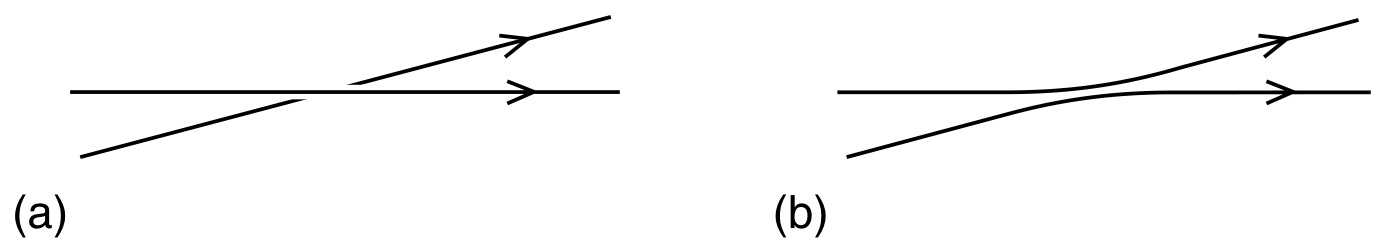
\includegraphics[width=0.8\textwidth]{figure/Fig13.4.jpg}
	\caption{(a) D-branes at relative angle. (b) Lower energy configuration.}
	\label{fig:13.4}
\end{figure}

In nonsupersymmetric configurations a tachyon can appear. For simplicity let only $\phi_1$ be nonzero, with $0 \le \phi_1 \le \pi$. The NS ground state energy is $-(1/2) + (\phi_1/2\pi)$, and the first excited state $\psi_{-1/2+(\phi_1/\pi)}^1\lvert 0\rangle_{\mathrm{NS}}$, which survives the GSO projection, has weight $-\phi_1/2\pi$. Including the energy from tension, the lightest state has
\begin{equation}
	m^2 = \frac{y_1^2}{4\pi^2{\alpha'}^2} - \frac{\phi_1}{2\pi\alpha'} \:, \quad 0 \le \phi_1 \le \pi \:. \label{13.4.27}
\end{equation}
This is negative if the separation is small enough. A special case is $\phi_1 = \pi$, when the 4-branes are antiparallel rather than parallel (a D4-brane and an anti-D4-brane). The NS--NS and R--R exchanges are then both attractive, and below the critical separation $y_1^2 = 2\pi^2\alpha'$ the cylinder amplitude diverges as $t \to \infty$. This is where the tachyon appears --- evidently it represents D4-brane/anti-D4-brane annihilation. Even when the D-branes are nearly parallel they can lower their energy by reconnecting as in Figure~\ref{fig:13.4}(b), and this is the physical origin of the instability. The decay has no end: the reconnected strings move apart indefinitely.
\begin{tcolorbox}[breakable]
	\begin{remark}
		\textbf{Conventions.} $\nu=\phi_1/\pi\in[0,1]$, the other three planes are unrotated, and the light-cone counting of the box after \eqref{13.4.8} is used. The mass-shell condition for a stretched open string is $m^2=(y_1/2\pi\alpha')^2+L_0^{\rm osc}/\alpha'$.

		\textit{NS ground-state energy.} In the rotated plane the complex boson has zero-point energy \eqref{13.4.17}. The NS fermion modes are shifted by the same $\nu$ from $\mathbb Z+\frac12$, so for a complex fermion with modes in $\mathbb Z+a$, the analogue of \eqref{13.4.17} with the opposite sign is $-\bigl[\frac1{24}-\frac12(a-\frac12)^2\bigr]$. This is $-\frac1{24}$ at $a=\frac12$ and $+\frac1{12}$ at $a=0$, as it should be. With $a=\frac12+\nu$,
		\begin{align*}
			E_{\rm plane} &= \Bigl[\frac1{24}-\frac12\Bigl(\nu-\frac12\Bigr)^2\Bigr]+\Bigl[-\frac1{24}+\frac12\nu^2\Bigr] \eqs{1} -\frac18+\frac\nu2 ,\\
			E_{\rm NS} &= 3\Bigl(-\frac18\Bigr)+\Bigl(-\frac18+\frac\nu2\Bigr) = -\frac12+\frac{\phi_1}{2\pi} .
		\end{align*}
		At (1), $\frac1{24}-\frac12\nu^2+\frac12\nu-\frac18-\frac1{24}+\frac12\nu^2=-\frac18+\frac\nu2$. The unrotated planes give $-\frac18$ each, from two NN or DD bosons and two NS fermions: $2(-\frac1{24}-\frac1{48})=-\frac18$.

		\textit{The lightest state.} The fermion mode $\psi^1_{-1/2+\nu}$ raises the energy by $\frac12-\nu$:
		\begin{equation*}
			L_0^{\rm osc} = -\frac12+\frac\nu2+\frac12-\nu = -\frac\nu2 = -\frac{\phi_1}{2\pi},\qquad
			m^2 = \frac{y_1^2}{4\pi^2{\alpha'}^2}-\frac{\phi_1}{2\pi\alpha'} ,
		\end{equation*}
		which is \eqref{13.4.27}. The NS ground state itself has the opposite GSO parity and is projected out, as for untwisted strings. At $\phi_1=\pi$ (brane and antibrane), $m^2<0$ for $y_1^2<4\pi^2\alpha'^2\cdot\frac{1}{2\alpha'}=2\pi^2\alpha'$, the critical separation quoted in the text. There the $t\to\infty$ region of the cylinder behaves as $e^{-2\pi t\alpha'm^2}$ and diverges.
	\end{remark}
\end{tcolorbox}


\section{D-Brane Interactions: Dynamics}

\subsection*{D-Brane Scattering}

For parallel static D-branes the potential energy is zero, but if they are in relative motion all supersymmetry is broken and there is a velocity-dependent force. This can be obtained by an analytic continuation of the static potential for rotated branes. Consider the case that only $\phi_1$ is nonzero, so the rotated brane satisfies $X^3 = X^2\tan\phi_1$. Analytically continue $X^2 \to \mi X'^0$ and let $\phi_1 = -\mi u$, with $u > 0$. Then
\begin{equation}
	X^3 = X'^0\tanh u \:, \label{13.5.1}
\end{equation}
which describes a D-brane moving with constant velocity. Continue also $X^0 \to -\mi X'^2$ to eliminate the spurious extra time coordinate. The interaction amplitude between the D-branes becomes
\begin{equation}
	\mathcal{A} = -\mi V_p\int_0^\infty \frac{\dif t}{t}\,(8\pi^2\alpha' t)^{-p/2}\exp\Bigl(-\frac{t y^2}{2\pi\alpha'}\Bigr)\frac{\vartheta_{11}(ut/2\pi, \mi t)^4}{\eta(\mi t)^9\,\vartheta_{11}(ut/\pi, \mi t)} \:, \label{13.5.2}
\end{equation}
where we have extended the result to general $p$ by using T-duality. It is also useful to give the modular transformation:
\begin{equation}
	\mathcal{A} = \frac{V_p}{(8\pi^2\alpha')^{p/2}}\int_0^\infty \frac{\dif t}{t}\,t^{(6-p)/2}\exp\Bigl(-\frac{t y^2}{2\pi\alpha'}\Bigr)\frac{\vartheta_{11}(\mi u/2\pi, \mi/t)^4}{\eta(\mi/t)^9\,\vartheta_{11}(\mi u/\pi, \mi/t)} \:. \label{13.5.3}
\end{equation}
\begin{tcolorbox}[breakable]
	\begin{remark}
		\textbf{Conventions.} The overall normalization of \eqref{13.5.2} is taken from the text. We derive its structure from \eqref{13.4.23} and then derive \eqref{13.5.3} from it. $\vartheta_{11}$ obeys \eqref{13.4.18a}--\eqref{13.4.18b} and is odd in $\nu$, and $\eta(\mi t)=t^{-1/2}\eta(\mi/t)$.

		\textit{\eqref{13.5.1}.} With $X^2=\mi X'^0$ and $\phi_1=-\mi u$, $\tan(-\mi u)=-\mi\tanh u$, so $X^3=X^2\tan\phi_1=\mi X'^0(-\mi\tanh u)=X'^0\tanh u$. This is a brane moving along $X^3$ with velocity $v=\tanh u<1$; $u$ is the rapidity.

		\textit{Structure of \eqref{13.5.2}.} With only $\phi_1\neq0$, \eqref{13.4.22} gives $\phi'_1=\phi'_2=\phi'_3=\phi'_4=\phi_1/2$, so the numerator of \eqref{13.4.23} is $\vartheta_{11}(\mi\phi_1t/2\pi,\mi t)^4$. The rotated plane gives the denominator $\vartheta_{11}(\mi\phi_1t/\pi,\mi t)$. Each of the three unrotated planes gives $\eta^{-3}$ by \eqref{13.4.24}--\eqref{13.4.25}, and their zero modes give the momentum and volume factors. Under $\phi_1=-\mi u$ the arguments become $\mi\phi_1t/\pi=ut/\pi$ and $ut/2\pi$, which are real, giving \eqref{13.5.2}.

		\textit{Modular transformation.} Solving \eqref{13.4.18b} for $\vartheta_{11}(\nu,\mi t)$ gives $\vartheta_{11}(\nu,\mi t)=\mi t^{-1/2}e^{-\pi\nu^2/t}\vartheta_{11}(-\mi\nu/t,\mi/t)$. Then
		\begin{align*}
			\vartheta_{11}\Bigl(\frac{ut}{2\pi},\mi t\Bigr)^4 &\eqs{1} t^{-2}e^{-u^2t/\pi}\,\vartheta_{11}\Bigl(\frac{\mi u}{2\pi},\frac{\mi}{t}\Bigr)^4, \\
			\vartheta_{11}\Bigl(\frac{ut}{\pi},\mi t\Bigr) &\eqs{2} -\mi t^{-1/2}e^{-u^2t/\pi}\,\vartheta_{11}\Bigl(\frac{\mi u}{\pi},\frac{\mi}{t}\Bigr),\\
			\frac{\vartheta_{11}(ut/2\pi,\mi t)^4}{\eta(\mi t)^9\vartheta_{11}(ut/\pi,\mi t)} \\ &\eqs{3} \frac{t^{-2}}{t^{-9/2}\cdot(-\mi)t^{-1/2}}\,\frac{\vartheta_{11}(\mi u/2\pi,\mi/t)^4}{\eta(\mi/t)^9\vartheta_{11}(\mi u/\pi,\mi/t)}\\
			&= \mi\,t^3\,\frac{\vartheta_{11}(\mi u/2\pi,\mi/t)^4}{\eta(\mi/t)^9\vartheta_{11}(\mi u/\pi,\mi/t)} .
		\end{align*}
		At (1), $(\mi t^{-1/2})^4=t^{-2}$, $4\pi(ut/2\pi)^2/t=u^2t/\pi$, and the sign of $-\mi u/2\pi$ drops out of the fourth power. At (2), $\pi(ut/\pi)^2/t=u^2t/\pi$, and oddness gives $\vartheta_{11}(-\mi u/\pi)=-\vartheta_{11}(\mi u/\pi)$. At (3), the exponentials cancel. Inserting into \eqref{13.5.2},
		\begin{align*}
			\mathcal A &= -\mi V_p\int_0^\infty\frac{\dif t}{t}(8\pi^2\alpha')^{-p/2}t^{-p/2}\cdot\mi t^3\,e^{-ty^2/2\pi\alpha'}\cdots\\ &= \frac{V_p}{(8\pi^2\alpha')^{p/2}}\int_0^\infty\frac{\dif t}{t}\,t^{(6-p)/2}e^{-ty^2/2\pi\alpha'}\cdots ,
		\end{align*}
		which is \eqref{13.5.3}.
	\end{remark}
\end{tcolorbox}

We can write this as an integral over the worldline:
\begin{equation}
	\mathcal{A} = -\mi\int_{-\infty}^{\infty}\dif\tau\:V(r(\tau), v) \:, \label{13.5.4}
\end{equation}
where
\begin{equation}
	r(\tau)^2 = y^2 + v^2\tau^2 \:, \quad v = \tanh u \:, \label{13.5.5}
\end{equation}
and
\begin{equation}
	V(r,v) = \frac{\mi}{2V_p(8\pi^2\alpha')^{(p+1)/2}}\int_0^\infty \dif t\:t^{(5-p)/2}\exp\Bigl(-\frac{t r^2}{2\pi\alpha'}\Bigr)\frac{(\tanh u)\,\vartheta_{11}(\mi u/2\pi, \mi/t)^4}{\eta(\mi/t)^9\,\vartheta_{11}(\mi u/\pi, \mi/t)} \:. \label{13.5.6}
\end{equation}

The interaction has a number of interesting properties. The first is that as $v \to 0$ (so that $u \to 0$), it vanishes as $v^4$ from the zeros of the theta functions. We expect only even powers of $v$ by time-reversal invariance. The vanishing of the $v^2$ interaction, like the vanishing of the static interaction, is a consequence of supersymmetry. The low energy field theory of the D-branes is a $\mathrm{U}(1)\times\mathrm{U}(1)$ supersymmetric gauge theory with 16 supersymmetries. What we are calculating is a correction to the effective action from integrating out massive states, strings stretched between the D-branes. The vanishing of the $v^2$ term is then consistent with the assertion that with 16 supersymmetries corrections to the kinetic term are forbidden --- the moduli space is flat. If we had instead taken $\phi_3 = \phi_4 = \pi/2$ so that $\#\mathrm{ND} = 4$, there would only be two zeros in the numerator and thus a $v^2$ interaction, consistent with the fact that kinetic corrections are allowed with 8 supercharges.

The interaction \eqref{13.5.6} is in general a complicated function of separation, but in an expansion in powers of the velocity the leading $\mathcal{O}(v^4)$ term is simple:
\begin{align}
	V(r,v) &= -\frac{v^4}{V_p(8\pi^2\alpha')^{(p+1)/2}}\int_0^\infty \dif t\:t^{(5-p)/2}\exp\Bigl(-\frac{t r^2}{2\pi\alpha'}\Bigr) + \mathcal{O}(v^6) \nonumber \\
	&= -\frac{v^4}{r^{7-p}}\frac{1}{V_p\alpha'^{p-3}}2^{2-2p}\pi^{(5-3p)/2}\Gamma\Bigl(\frac{7-p}{2}\Bigr) + \mathcal{O}(v^6) \:. \label{13.5.7}
\end{align}
At long distances this is in agreement with low energy supergravity. It is also the leading behavior if we expand in powers of $1/r$ rather than $v$.
\begin{tcolorbox}[breakable]
	\begin{remark}
		\textbf{Conventions.} Write the closed-channel ratio in \eqref{13.5.3} as $F(u,t)\equiv\vartheta_{11}(\mi u/2\pi,\mi/t)^4/[\eta(\mi/t)^9\vartheta_{11}(\mi u/\pi,\mi/t)]$. $V(r,v)$ is the full potential between the branes, so it is proportional to the brane volume $V_p$.

		\textit{From \eqref{13.5.3} to \eqref{13.5.4}--\eqref{13.5.6}.} The Gaussian integral over the trajectory $r^2=y^2+v^2\tau^2$ gives
		\begin{equation*}
			\int_{-\infty}^\infty\dif\tau\,e^{-tr(\tau)^2/2\pi\alpha'} = e^{-ty^2/2\pi\alpha'}\,\frac1v\Bigl(\frac{2\pi^2\alpha'}{t}\Bigr)^{1/2} .
		\end{equation*}
		So if $V(r,v)=C\int\dif t\,t^{a}e^{-tr^2/2\pi\alpha'}F$, then $-\mi\int\dif\tau\,V=-\mi C\,v^{-1}(2\pi^2\alpha')^{1/2}\int\dif t\,t^{a-1/2}e^{-ty^2/2\pi\alpha'}F$. Matching to \eqref{13.5.3},
		\begin{align*}
			a-\tfrac12 &= \tfrac{6-p}{2}-1 \;\Longrightarrow\; a=\tfrac{5-p}{2},\qquad
			C \eqs{1} \mi v\,V_p\,(8\pi^2\alpha')^{-p/2}(2\pi^2\alpha')^{-1/2} \eqs{2} \frac{2\mi\,V_p\tanh u}{(8\pi^2\alpha')^{(p+1)/2}} .
		\end{align*}
		At (1), $-\mi C/v=\ldots$ was solved using $1/(-\mi)=\mi$. At (2), $(2\pi^2\alpha')^{-1/2}=2(8\pi^2\alpha')^{-1/2}$ and $v=\tanh u$. The power $t^{(5-p)/2}$ agrees with \eqref{13.5.6}, but the prefactor should be $2\mi V_p\tanh u/(8\pi^2\alpha')^{(p+1)/2}$: the $V_p$ belongs in the numerator and the factor is $2\mi$, not $\mi/2$.

		\textit{Small-velocity expansion \eqref{13.5.7}.} For small argument, \eqref{13.4.18a} gives $\vartheta_{11}(\nu,\tau)=-2\pi\nu\,\eta(\tau)^3+\mathcal O(\nu^3)$, since $q^{1/8}\prod(1-q^m)^3=\eta^3$. Hence, uniformly in $t$,
		\begin{align*}
			F(u,t) &= \frac{(-2\pi\cdot\mi u/2\pi)^4\eta^{12}}{\eta^9\,(-2\pi\cdot\mi u/\pi)\,\eta^3}\bigl(1+\mathcal O(u^2)\bigr)\\ &= \frac{u^4}{-2\mi u} = \frac{\mi}{2}u^3+\mathcal O(u^5),\\
			V(r,v) &\eqs{3} \frac{2\mi V_p\tanh u}{(8\pi^2\alpha')^{(p+1)/2}}\cdot\frac{\mi}{2}u^3\int_0^\infty\dif t\,t^{(5-p)/2}e^{-tr^2/2\pi\alpha'}\\ &= -\frac{v^4V_p}{(8\pi^2\alpha')^{(p+1)/2}}\int_0^\infty\dif t\,t^{(5-p)/2}e^{-tr^2/2\pi\alpha'}+\mathcal O(v^6).
		\end{align*}
		At (3), $u^3\tanh u=v^4+\mathcal O(v^6)$. This is the first line of \eqref{13.5.7} with $V_p$ in the numerator; the coefficient 1 confirms the corrected prefactor $2\mi$. The four zeros of the numerator give $u^4$, and the single zero of the denominator removes one power, which with the $\tanh u$ gives $v^4$. With $\phi_3=\phi_4=\pi/2$ ($\#\mathrm{ND}=4$) two of the four $\phi'_a$ no longer vanish at $u=0$, so only two numerator zeros remain and the result starts at $v^2$. Doing the $t$ integral,
		\begin{align*}
			\int_0^\infty\dif t\,t^{(5-p)/2}e^{-tr^2/2\pi\alpha'} &= \Gamma\Bigl(\frac{7-p}{2}\Bigr)\Bigl(\frac{2\pi\alpha'}{r^2}\Bigr)^{(7-p)/2},\\
			\frac{(2\pi\alpha')^{(7-p)/2}}{(8\pi^2\alpha')^{(p+1)/2}} &\eqs{4} 2^{2-2p}\pi^{(5-3p)/2}{\alpha'}^{3-p},\\
			V(r,v) &= -\frac{v^4}{r^{7-p}}\,V_p\,{\alpha'}^{3-p}\,2^{2-2p}\pi^{(5-3p)/2}\,\Gamma\Bigl(\frac{7-p}{2}\Bigr)+\mathcal O(v^6).
		\end{align*}
		At (4), the powers of 2 are $\frac{7-p}{2}-\frac{3(p+1)}{2}=2-2p$ and of $\pi$ are $\frac{7-p}{2}-(p+1)=\frac{5-3p}{2}$. The numbers agree with the second line of \eqref{13.5.7}, but the volume factor there should be $V_p/\alpha'^{p-3}$ rather than $1/(V_p\alpha'^{p-3})$. The $r^{p-7}=r^{2-(9-p)}$ fall-off is the Green function in the $9-p$ transverse dimensions, as for supergravity exchange.
	\end{remark}
\end{tcolorbox}

In general the behavior of $V(r,v)$ as $r \to 0$ is quite different from the behavior as $r \to \infty$. The $r$-dependence of the integral \eqref{13.5.6} arises from the factor $\exp(-t r^2/2\pi\alpha')$, so that $t \approx 2\pi\alpha'/r^2$ governs the behavior at given $r$. Large $r$ corresponds to small $t$, where the asymptotic behavior is given by tree-level exchange of light closed strings --- hence the agreement with classical supergravity. Small $r$ corresponds to large $t$, where the asymptotic behavior is given by a loop of light open strings. The crossover is at $r^2 \sim 2\pi\alpha'$. This is as we expect: string theory modifies gravity at distances below the string scale.

To obtain the small-$r$ behavior of the scattering amplitude \eqref{13.5.6}, take the large-$t$ limit without expanding in $v$ to obtain:
\begin{equation}
	V(r,v) \approx -2V_p\int_0^\infty \frac{\dif t}{(8\pi^2\alpha' t)^{(p+1)/2}}\exp\Bigl(-\frac{t r^2}{2\pi\alpha'}\Bigr)\tanh u\,\frac{\sin^4(ut/2)}{\sin(ut)} \:. \label{13.5.8}
\end{equation}
\begin{tcolorbox}[breakable]
	\begin{remark}
		The large-$t$ limit is simplest in the open-string form \eqref{13.5.2}, where $q=e^{-2\pi t}\to0$. By \eqref{13.4.18a} with real $\nu$, $\vartheta_{11}(\nu,\mi t)\to-2q^{1/8}\sin\pi\nu$, and $\eta(\mi t)\to q^{1/24}$, so
		\begin{align*}
			\frac{\vartheta_{11}(ut/2\pi,\mi t)^4}{\eta^9\,\vartheta_{11}(ut/\pi,\mi t)} &\;\to\; \frac{16\,q^{1/2}\sin^4(ut/2)}{q^{9/24}\,(-2q^{1/8})\sin(ut)} \eqs{1} -8\,\frac{\sin^4(ut/2)}{\sin(ut)} ,\\
			\mathcal A &\approx 8\mi V_p\int_0^\infty\frac{\dif t}{t}(8\pi^2\alpha't)^{-p/2}e^{-ty^2/2\pi\alpha'}\frac{\sin^4(ut/2)}{\sin(ut)} .
		\end{align*}
		At (1), the powers of $q$ cancel, $\frac12-\frac38-\frac18=0$: only the massless open strings survive at large $t$, and these are the light stretched strings. Converting to a potential with $e^{-ty^2/2\pi\alpha'}=v\,(t/2\pi^2\alpha')^{1/2}\int\dif\tau\,e^{-tr^2/2\pi\alpha'}$ (the inverse of the Gaussian integral in the previous box) and $\mathcal A=-\mi\int\dif\tau\,V$,
		\begin{align*}
			V(r,v) &\approx -8V_p\,v\int_0^\infty\frac{\dif t}{t}(8\pi^2\alpha't)^{-p/2}\,\frac{2t^{1/2}}{(8\pi^2\alpha')^{1/2}}\,e^{-tr^2/2\pi\alpha'}\frac{\sin^4(ut/2)}{\sin(ut)}\\
			&\eqs{2} -16V_p\int_0^\infty\frac{\dif t}{(8\pi^2\alpha't)^{(p+1)/2}}\,e^{-tr^2/2\pi\alpha'}\tanh u\,\frac{\sin^4(ut/2)}{\sin(ut)} .
		\end{align*}
		At (2), $t^{-1}t^{-p/2}t^{1/2}=t^{-(p+1)/2}$ and $v=\tanh u$. The coefficient is 16, not the printed 2. As a check, expanding for small $u$, $\sin^4(ut/2)/\sin(ut)\approx u^3t^3/16$, so this gives $-v^4V_p(8\pi^2\alpha')^{-(p+1)/2}\int\dif t\,t^{(5-p)/2}e^{-tr^2/2\pi\alpha'}$, exactly the corrected \eqref{13.5.7}. With the printed 2 it would be $\frac18$ of that. The large-$t$ region is not required to have small $u t$, so \eqref{13.5.8} keeps the full dependence on $ut$.

		\textit{\eqref{13.5.9}--\eqref{13.5.12}.} The Gaussian localizes $t\approx2\pi\alpha'/r^2$, so the argument of the sines is $ut\approx2\pi\alpha'v/r^2$. The $v^4$ expansion fails and the oscillations set in when this is of order one, at $r^2\approx\alpha'v$, which is \eqref{13.5.9}. The encounter lasts $\delta t\approx r/v$, so $\delta x\,\delta t\approx r^2/v\approx\alpha'$, which is \eqref{13.5.10}. A D0-brane of mass $m=\tau_0=1/(g\alpha'^{1/2})$ from \eqref{13.3.23} with velocity spread $\delta v$ has $\delta p=m\,\delta v$, so $\delta x\gtrsim1/(m\,\delta v)$, which is \eqref{13.5.11}. Taking $\delta v\sim v$, the total uncertainty is
		\begin{equation*}
			f(v) = \alpha'^{1/2}\Bigl(v^{1/2}+\frac gv\Bigr),\qquad f'(v)=0 \;\Longrightarrow\; \frac12v^{-1/2}=\frac g{v^2} \;\Longrightarrow\; v=(2g)^{2/3}\sim g^{2/3},
		\end{equation*}
		and then $f\sim\alpha'^{1/2}(g^{1/3}+g^{1/3})\sim g^{1/3}\alpha'^{1/2}$, which is \eqref{13.5.12}.
	\end{remark}
\end{tcolorbox}
Since $t \approx 2\pi\alpha'/r^2$ and $v \approx u$, the arguments of the sines are $u t \approx 2\pi\alpha' v/r^2$. No matter how small $v$ is, the $v^4$ term will cease to dominate at small enough $r$. The oscillations of the integrand then smooth the small-$r$ behavior on a scale $u t \approx 1$. The effective scale probed by the scattering is
\begin{equation}
	r \approx \alpha'^{1/2}v^{1/2} \:. \label{13.5.9}
\end{equation}
A small-velocity D-brane probe is thus sensitive to distances shorter than the string scale! This is in contrast to the behavior seen in string scattering at weak coupling, but fits nicely with the understanding of strongly coupled strings.

A slower D-brane probes shorter distances, but the scattering process takes longer, $\delta t \approx r/v$. Then
\begin{equation}
	\delta x\,\delta t \gtrsim \alpha' \:. \label{13.5.10}
\end{equation}
This is a suggestion for a new uncertainty relation involving only the coordinates, an indication of `noncommutative geometry' connected with the promotion of D-brane collective coordinates to matrices.

For a pointlike D0-brane probe there is a minimum distance that can be measured by scattering. The wavepacket in which it is prepared satisfies:
\begin{equation}
	\delta x \gtrsim \frac{1}{m\delta v} = \frac{g\alpha'^{1/2}}{\delta v} \:. \label{13.5.11}
\end{equation}
The combined uncertainties \eqref{13.5.9} and \eqref{13.5.11} are minimized by $v \approx g^{2/3}$, for which
\begin{equation}
	\delta x \gtrsim g^{1/3}\alpha'^{1/2} \:. \label{13.5.12}
\end{equation}

\subsection*{D0-Brane Quantum Mechanics}

The nonrelativistic effective Lagrangian for $n$ D0-branes is
\begin{equation}
	L = \operatorname{Tr}\biggl(\frac{1}{2g\alpha'^{1/2}}D_0 X^i D_0 X^i + \frac{1}{4g\alpha'^{1/2}(2\pi\alpha')^2}[X^i,X^j]^2 - \frac{\mi}{2}\lambda D_0\lambda + \frac{1}{4\pi\alpha'}\lambda\Gamma^0\Gamma^i[X^i,\lambda]\biggr) \:. \label{13.5.13}
\end{equation}
The first term is the usual nonrelativistic kinetic energy with $m = \tau_0 = 1/(g\alpha'^{1/2})$, dropping the constant rest mass $n\tau_0$. The coefficients of the other terms are most easily obtained by T-duality from the ten-dimensional super-Yang--Mills action (B.6.13), with $A_i \to X^i/(2\pi\alpha')$. We have taken a basis in which the fermionic field $\lambda$ is Hermitian, and rescaled $\lambda$ to obtain a canonical kinetic term. The index $i$ runs over the nine spatial dimensions. The gauge field $A_0$ has no kinetic term but remains in the covariant derivatives. It couples to the $\mathrm{U}(n)$ charges, so its equation of motion amounts to the constraint that only $\mathrm{U}(n)$-invariant states are allowed. Only terms with at most two powers of the velocity have been kept, not the full Born--Infeld action.

The Hamiltonian is
\begin{equation}
	H = \operatorname{Tr}\biggl(\frac{g\alpha'^{1/2}}{2}p_i p_i - \frac{1}{16\pi^2 g\alpha'^{5/2}}[X^i,X^j]^2 - \frac{1}{4\pi\alpha'}\lambda\Gamma^0\Gamma^i[X^i,\lambda]\biggr) \:. \label{13.5.14}
\end{equation}
Note that the potential is positive because $[X^i,X^j]$ is anti-Hermitian. The canonical momentum, like the coordinate, is a matrix:
\begin{equation}
	[p_i^{ab}, X_j^{cd}] = -\mi\delta_{ij}\delta^{ad}\delta^{bc} \:. \label{13.5.15}
\end{equation}

Now we define
\begin{equation}
	X^i = g^{1/3}\alpha'^{1/2}Y^i \:, \label{13.5.16}
\end{equation}
so that also $p_i = p_{Y^i}/(g^{1/3}\alpha'^{1/2})$. The Hamiltonian becomes
\begin{equation}
	H = \frac{g^{1/3}}{\alpha'^{1/2}}\operatorname{Tr}\biggl(\frac{1}{2}p_{Y^i}p_{Y^i} - \frac{1}{16\pi^2}[Y^i,Y^j]^2 - \frac{1}{4\pi}\lambda\Gamma^0\Gamma^i[Y^i,\lambda]\biggr) \:. \label{13.5.17}
\end{equation}
The parameters $g$ and $\alpha'$ now appear only in the overall normalization. It follows that the wavefunctions are independent of the parameters when expressed in terms of the variables $Y^i$. In terms of the original coordinates $X^i$ their characteristic size scales as $g^{1/3}\alpha'^{1/2}$, the same scale \eqref{13.5.12} found above. The energies scale as $g^{1/3}/\alpha'^{1/2}$ from the overall normalization of $H$, and the characteristic times scale as the inverse of this, recovering the relation \eqref{13.5.10}.
\begin{tcolorbox}[breakable]
	\begin{remark}
		\textbf{Conventions.} We start from the bosonic part of ten-dimensional SYM, $-\frac{1}{4g_{\rm D0}^2}\int\operatorname{Tr}F_{MN}F^{MN}$ with $F_{MN}=\partial_MA_N-\partial_NA_M+\mi[A_M,A_N]$, reduced to $0+1$ dimensions with $A_i\to X^i/2\pi\alpha'$. The D0-brane coupling is \eqref{13.3.25} at $p=0$, $g_{\rm D0}^2=(2\pi)^{-2}g\alpha'^{-3/2}$, so $\frac1{g_{\rm D0}^2}=\frac{(2\pi)^2\alpha'^{3/2}}{g}$. The fermion normalization is taken from the text.

		\textit{Bosonic terms of \eqref{13.5.13}.}
		\begin{align*}
			F_{0i}=\frac{D_0X^i}{2\pi\alpha'},\ \ F_{ij}=\frac{\mi[X^i,X^j]}{(2\pi\alpha')^2}
			\;&\Longrightarrow\;
			-\frac1{4g_{\rm D0}^2}\operatorname{Tr}\bigl(2F_{0i}F^{0i}+F_{ij}F^{ij}\bigr)\\
			&\eqs{1} \frac{1}{2g_{\rm D0}^2}\frac{\operatorname{Tr}(D_0X^i)^2}{(2\pi\alpha')^2}+\frac{1}{4g_{\rm D0}^2}\frac{\operatorname{Tr}[X^i,X^j]^2}{(2\pi\alpha')^4},\\
			\frac{1}{2g_{\rm D0}^2(2\pi\alpha')^2} &= \frac{(2\pi)^2\alpha'^{3/2}}{2g(2\pi)^2\alpha'^2}=\frac{1}{2g\alpha'^{1/2}},\\
			\frac{1}{4g_{\rm D0}^2(2\pi\alpha')^4}&=\frac{1}{4g\alpha'^{1/2}(2\pi\alpha')^2} .
		\end{align*}
		At (1), $F^{0i}=-F_{0i}$ and $(\mi[X^i,X^j])^2=-[X^i,X^j]^2$. Both coefficients are those of \eqref{13.5.13}, and the first is $\frac12m$ with $m=\tau_0=1/(g\alpha'^{1/2})$ from \eqref{13.3.23}.

		\textit{Hamiltonian \eqref{13.5.14}.} With $p_i=\partial L/\partial(D_0X^i)=D_0X^i/(g\alpha'^{1/2})$ (as matrices, $p^{ab}_i$ conjugate to $X^{ba}_i$, which gives \eqref{13.5.15}), the Legendre transform flips the sign of every term without time derivatives:
		\begin{equation*}
			H=\operatorname{Tr}\Bigl(\frac{g\alpha'^{1/2}}{2}p_ip_i-\frac{1}{4g\alpha'^{1/2}(2\pi\alpha')^2}[X^i,X^j]^2-\frac1{4\pi\alpha'}\lambda\Gamma^0\Gamma^i[X^i,\lambda]\Bigr),
		\end{equation*}
		and $4(2\pi\alpha')^2\alpha'^{1/2}=16\pi^2\alpha'^{5/2}$, which is \eqref{13.5.14}. The first-order fermion kinetic term does not contribute to $H$. Since $[X^i,X^j]^\dagger=-[X^i,X^j]$, $\operatorname{Tr}[X^i,X^j]^2=-\operatorname{Tr}\bigl([X^i,X^j]^\dagger[X^i,X^j]\bigr)\le0$, so the potential $-\operatorname{Tr}[X,X]^2/16\pi^2g\alpha'^{5/2}$ is non-negative. It vanishes exactly on commuting matrices, which are the flat directions.

		\textit{Scaling \eqref{13.5.17}.} With $X=\ell Y$, $p=p_Y/\ell$ and $\ell=g^{1/3}\alpha'^{1/2}$, which preserves \eqref{13.5.15},
		\begin{align*}
			\frac{g\alpha'^{1/2}}{2}\frac{p_Y^2}{\ell^2} &= \frac{g^{1/3}}{\alpha'^{1/2}}\,\frac{p_Y^2}{2},\\
			\frac{\ell^4}{16\pi^2g\alpha'^{5/2}}[Y,Y]^2 &= \frac{g^{1/3}}{\alpha'^{1/2}}\,\frac{[Y,Y]^2}{16\pi^2},\\
			\frac{\ell}{4\pi\alpha'}\lambda\Gamma^0\Gamma^i[Y^i,\lambda] &= \frac{g^{1/3}}{\alpha'^{1/2}}\,\frac{\lambda\Gamma^0\Gamma^i[Y^i,\lambda]}{4\pi} .
		\end{align*}
		The three terms acquire the same prefactor because $g\alpha'^{1/2}\ell^{-2}=\ell^4/(g\alpha'^{5/2})=\ell/\alpha'$ exactly when $\ell^3=g\alpha'^{3/2}$. That is the only way to choose $\ell$, and it gives the length $g^{1/3}\alpha'^{1/2}$ of \eqref{13.5.12}. The energy scale is $g^{1/3}/\alpha'^{1/2}$, and time scale $\times$ length scale $=\alpha'^{1/2}g^{-1/3}\cdot g^{1/3}\alpha'^{1/2}=\alpha'$, which is \eqref{13.5.10}.
	\end{remark}
\end{tcolorbox}

Recall from the discussion of D-brane scattering that at distances less than the string scale only the lightest open string states contribute. In this regime the cylinder amplitude reduces to a loop amplitude in the low energy field theory \eqref{13.5.13}.

\subsection*{The $\#\mathrm{ND} = 4$ System}

Another low energy action with many applications is that for a D$p$-brane and D$p'$-brane with relative $\#\mathrm{ND} = 4$. There are three kinds of light strings: $p$-$p$, $p$-$p'$, and $p'$-$p'$, with ends on the respective D-branes. We will consider explicitly the case $p = 5$ and $p' = 9$, where we can take advantage of the $\mathrm{SO}(5,1)\times\mathrm{SO}(4)$ spacetime symmetry; all other cases are related to this by T-duality.

The 5-5 and 9-9 strings are the same as those that arise on a single D-brane. The new feature is the 5-9 strings; let us study their massless spectrum. The NS zero-point energy is zero. The moding of the fermions differs from that of the bosons by $1/2$, so there are four periodic worldsheet fermions $\psi^m$, namely those in the ND directions $m = 6, 7, 8, 9$. The four zero modes then generate $2^{4/2} = 4$ degenerate ground states, which we label by their spins in the $(6,7)$ and $(8,9)$ planes:
\begin{equation}
	\lvert s_3, s_4\rangle_{\mathrm{NS}} \:, \label{13.5.18}
\end{equation}
with $s_3, s_4 = \pm 1/2$. Now we need to impose the GSO projection. This was defined in \eqref{10.2.22} in terms of $s_a$, so that with the extra sign from the ghosts it is
\begin{equation}
	-\exp\bigl(\pi\mi(s_3 + s_4)\bigr) = +1 \quad \Longrightarrow \quad s_3 = s_4 \:. \label{13.5.19}
\end{equation}
In terms of symmetries, the four states \eqref{13.5.18} are invariant under $\mathrm{SO}(5,1)$ and form spinors $\mathbf{2} + \mathbf{2}'$ of the `internal' $\mathrm{SO}(4)$, and only the $\mathbf{2}$ survives the GSO projection. In the R sector, of the transverse fermions $\psi^i$ only those with $i = 2, 3, 4, 5$ are periodic, so there are again four ground states:
\begin{equation}
	\lvert s_1, s_2\rangle_{\mathrm{R}} \:. \label{13.5.20}
\end{equation}
The GSO projection does not have an extra sign in the R sector so it requires $s_1 = -s_2$. The surviving spinors are invariant under the internal $\mathrm{SO}(4)$ and form a $\mathbf{2}'$ of the $\mathrm{SO}(4)$ little group of a massless particle.
\begin{tcolorbox}[breakable]
	\begin{remark}
		\textbf{Conventions.} Light-cone directions are $0,1$; the NN directions transverse to the light cone are $2,3,4,5$, and the ND directions are $6,7,8,9$. As in \eqref{10.2.22}, $\exp(\pi\mi F)$ acts on a zero-mode ground state as $\exp\bigl(\pi\mi\sum s_a\bigr)$ over the planes with zero modes, with an extra $-1$ in the NS sector from the ghosts. The physical states have $\exp(\pi\mi F)=+1$.

		\textit{NS sector.} By \eqref{13.4.8} with $\#\mathrm{ND}=4$, the zero-point energy is $-\frac12+\frac48=0$. The NS fermions $\psi^{6,7,8,9}$ are integer-moded and have zero modes, and $\{\psi^m_0,\psi^n_0\}=\delta^{mn}$ generates a Clifford algebra with $2^{4/2}=4$ states $|s_3,s_4\rangle$ ($s_3$ for the $(6,7)$ plane, $s_4$ for $(8,9)$). Then
		\begin{equation*}
			-e^{\pi\mi(s_3+s_4)}=+1 \;\Longleftrightarrow\; s_3+s_4\in\{\pm1\} \;\Longleftrightarrow\; s_3=s_4 .
		\end{equation*}
		These two states have $\prod2s=+1$ in the internal SO(4), which is one of its two-dimensional spinors, the $\mathbf 2$. The internal SO(4) is the rotation group of the ND directions; SO(4)$\,\cong\,$SU(2)$\times$SU(2), and its spinors are $\mathbf2=(\mathbf2,\mathbf1)$ and $\mathbf2'=(\mathbf1,\mathbf2)$. They carry no spacetime spin, so they are scalars of SO(5,1).

		\textit{R sector.} The zero-point energy is $0$, and the integer-moded fermions are now those in the NN directions, $\psi^{2,3,4,5}$, giving $|s_1,s_2\rangle$ with $s_1$ for $(2,3)$ and $s_2$ for $(4,5)$. With no ghost sign,
		\begin{equation*}
			e^{\pi\mi(s_1+s_2)}=+1 \;\Longleftrightarrow\; s_1+s_2=0 \;\Longleftrightarrow\; s_1=-s_2 ,
		\end{equation*}
		which is a two-component spinor of the SO(4) little group of a massless particle in six dimensions, of definite chirality ($\prod2s=-1$, the $\mathbf2'$). The 5-9 string is oriented, so its fields are complex, and its massless content is a doublet $\chi_i$ of complex scalars under the internal SU(2) plus one chiral spinor: half a hypermultiplet. The 9-5 strings supply the conjugate half. Which chirality survives in each sector depends on the sign conventions in \eqref{10.2.22}; the physical point is that the GSO projection keeps one of the two in each sector.
	\end{remark}
\end{tcolorbox}

The system has six-dimensional Lorentz invariance and eight unbroken supersymmetries, so we can classify it by $d = 6, N = 1$ supersymmetry (section B.7). The massless content of the 5-9 spectrum amounts to half of a hypermultiplet. The other half comes from strings of opposite orientation, 9-5. The action is fully determined by supersymmetry and the charges; we write the bosonic part:
\begin{equation}
	S = -\frac{1}{4g_{\mathrm{D}9}^2}\int \dif^{10}x\,F_{MN}F^{MN} - \frac{1}{4g_{\mathrm{D}5}^2}\int \dif^6 x\,F'_{MN}F'^{MN} - \int \dif^6 x\,\Bigl(D_\mu\chi^\dagger D^\mu\chi + \frac{g_{\mathrm{D}5}^2}{2}\sum_{A=1}^3(\chi_i^\dagger\sigma_{ij}^A\chi_j)^2\Bigr) \:. \label{13.5.21}
\end{equation}
The integrals run respectively over the 9-brane and the 5-brane, with $M = 0,\dots,9$, $\mu = 0,\dots,5$, and $m = 6,\dots,9$. The covariant derivative is $D_\mu = \del_\mu + \mi A_\mu - \mi A'_\mu$ with $A_\mu$ and $A'_\mu$ the 9-brane and 5-brane gauge fields. The field $\chi_i$ is a doublet describing the hypermultiplet scalars. The 5-9 strings have one endpoint on each D-brane so $\chi$ carries charges $+1$ and $-1$ under the respective symmetries. The gauge couplings $g_{\mathrm{D}p}$ were given in \eqref{13.3.25}. We are using a condensed notation:
\begin{equation}
	A'_M \longrightarrow A'_\mu \:, \quad X'^m/(2\pi\alpha') \:. \label{13.5.22}
\end{equation}
The massless 5-5 (and also 9-9) strings separate into $d = 6, N = 1$ vector and hypermultiplets. The final potential term is the 5-5 D-term required by supersymmetry. One might have expected a 9-9 D-term as well by T-duality, but this is inversely proportional to the volume of the D9-brane in the $(6,7,8,9)$-directions, which we have taken to be infinite.

Under T-dualities in any of the ND directions, one obtains $(p, p') = (8,6), (7,7), (6,8)$, or $(5,9)$, but the intersection of the branes remains $(5+1)$-dimensional and the $p$-$p'$ strings live on the intersection with action \eqref{13.5.21}. T-dualities in $r$ NN directions give $(p, p') = (9-r, 5-r)$. The vector components in the dualized directions become collective coordinates as usual:
\begin{equation}
	A_i \longrightarrow X^i/(2\pi\alpha') \:, \quad A'_i \longrightarrow X'^i/(2\pi\alpha') \:. \label{13.5.23}
\end{equation}
The term $D_i\chi^\dagger D_i\chi$ then becomes
\begin{equation}
	\biggl(\frac{X^i - X'^i}{2\pi\alpha'}\biggr)^2\chi^\dagger\chi \:. \label{13.5.24}
\end{equation}
This just reflects the fact that when the $(9-r)$-brane and $(5-r)$-brane are separated, the strings stretched between them become massive. The action for several branes of each type is given by the non-Abelian extension.
\begin{tcolorbox}[breakable]
	\begin{remark}
		In a dualized direction $i$ the fields no longer depend on $x^i$, so $\partial_i\chi=0$, and \eqref{13.5.23} turns the covariant derivative into
		\begin{align*}
			D_i\chi = \bigl(\partial_i+\mi A_i-\mi A'_i\bigr)\chi \eqs{1} \frac{\mi\,(X^i-X'^i)}{2\pi\alpha'}\chi
			\;\Longrightarrow\; D_i\chi^\dagger D_i\chi = \Bigl(\frac{X^i-X'^i}{2\pi\alpha'}\Bigr)^2\chi^\dagger\chi ,
		\end{align*}
		which is \eqref{13.5.24}. At (1), the charges $+1$ and $-1$ of $\chi$ under the two gauge groups were used. The mass term in $-\int D\chi^\dagger D\chi$ is $m^2=(\Delta X/2\pi\alpha')^2$, exactly the mass of a string of tension $1/2\pi\alpha'$ stretched over the separation $\Delta X$. This is the same stretching term as $e^{-ty^2/2\pi\alpha'}$ in the cylinder amplitudes, since $e^{-2\pi t\alpha'm^2}=e^{-t\Delta X^2/2\pi\alpha'}$. Under T-duality along NN directions, $(p,p')\to(9-r,5-r)$, and the ND count stays 4 because NN directions become DD, not ND.
	\end{remark}
\end{tcolorbox}


\section{D-Brane Interactions: Bound States}

Bound states of D-branes with strings and with each other, and supersymmetric bound states in particular, present a number of interesting dynamical problems. Further, these bound states will play an important role in the next chapter in our attempts to deduce the strongly coupled behavior of string theory.

\subsection*{$(p,q)$ String Bound States}

The first case we consider is a state with $p$ F-strings and $q$ D-strings in the IIB theory, all at rest and aligned along the 1-direction. For a state with these charges, the supersymmetry algebra \eqref{13.2.9} becomes
\begin{equation}
	\frac{1}{2}\begin{Bmatrix} Q_\alpha \\ \tilde{Q}_\alpha \end{Bmatrix}\begin{Bmatrix} Q_\beta^\dagger & \tilde{Q}_\beta^\dagger \end{Bmatrix} = M\delta_{\alpha\beta}\begin{pmatrix} 1 & 0 \\ 0 & 1 \end{pmatrix} + \frac{L_1}{2\pi\alpha'}(\Gamma^0\Gamma^1)_{\alpha\beta}\begin{pmatrix} p & q/g \\ q/g & -p \end{pmatrix} \:, \label{13.6.1}
\end{equation}
where $L_1$ is the length of the system. The eigenvalues of $\Gamma^0\Gamma^1$ are $\pm 1$, so those of the right-hand side are
\begin{equation}
	M \pm \frac{L_1(p^2 + q^2/g^2)^{1/2}}{2\pi\alpha'} \:. \label{13.6.2}
\end{equation}
The left-hand side of the algebra is positive --- its expectation value in any state is a matrix with positive eigenvalues. This implies a BPS bound on the total energy per unit length:
\begin{equation}
	\frac{M}{L_1} \ge \frac{(p^2 + q^2/g^2)^{1/2}}{2\pi\alpha'} \:. \label{13.6.3}
\end{equation}
This inequality is saturated by the F-string, which has $(p,q) = (1,0)$, and by the D-string, with $(p,q) = (0,1)$.
\begin{tcolorbox}[breakable]
	\begin{remark}
		\textbf{Conventions.} As in the BPS box after \eqref{13.2.10}: a Majorana basis, $\mathcal C=\Gamma^0$, and a static state at rest with $P^0=M$. The strings lie along $x^1$ with length $L_1$, so $Q^1_{\rm NS}=pL_1$ and the D-string charge is $qL_1$, with charges normalized to one per unit length as stated below \eqref{13.2.9}.

		\textit{The entries of \eqref{13.6.1}.} By \eqref{13.2.9a}--\eqref{13.2.9b} the diagonal blocks are $M\delta_{\alpha\beta}\pm\frac{pL_1}{2\pi\alpha'}(\Gamma^0\Gamma^1)_{\alpha\beta}$, with opposite signs for $Q$ and $\tilde Q$. By \eqref{13.2.9c} the off-diagonal block is $\tau_1Q_{\rm R}^1(\Gamma^0\beta_1)$, and $\tau_{\rm D1}=1/(2\pi\alpha'g)$ from \eqref{13.3.23}, so it is $\frac{qL_1}{2\pi\alpha' g}$ times a matrix that can be brought to $\Gamma^0\Gamma^1$ by a redefinition of $\tilde Q$ (as in \eqref{13.2.10}).

		\textit{Eigenvalues.} The two factors commute and act on different indices, so the eigenvalues of the product are products of eigenvalues:
		\begin{align*}
			(\Gamma^0\Gamma^1)^2 &= -\Gamma^0\Gamma^0\Gamma^1\Gamma^1 \eqs{1} 1 ,\\
			\det\begin{pmatrix} p-\lambda & q/g \\ q/g & -p-\lambda\end{pmatrix} &= \lambda^2-p^2-\frac{q^2}{g^2}=0 \;\Longrightarrow\; \lambda=\pm\Bigl(p^2+\frac{q^2}{g^2}\Bigr)^{1/2} .
		\end{align*}
		At (1), $(\Gamma^0)^2=-1$ and $(\Gamma^1)^2=+1$; $\Gamma^0\Gamma^1$ is traceless, so its eigenvalues $\pm1$ each occur 16 times. The right-hand side of \eqref{13.6.1} therefore has eigenvalues $M\pm L_1(p^2+q^2/g^2)^{1/2}/2\pi\alpha'$, which is \eqref{13.6.2}. The left-hand side has the form $\frac12\sum\mathcal Q\mathcal Q^\dagger$, whose expectation value is $\frac12\|\mathcal Q^\dagger|\psi\rangle\|^2\ge0$, so the smaller eigenvalue must be non-negative, which is \eqref{13.6.3}. The bound is saturated when half the 32 supercharges annihilate the state. For $(1,0)$ it gives $1/2\pi\alpha'=\tau_{\rm F1}$, and for $(0,1)$ it gives $1/2\pi\alpha'g=\tau_{\rm D1}$, the known tensions.
	\end{remark}
\end{tcolorbox}

For one F-string and one D-string, the total energy per unit length is
\begin{equation}
	\tau_{(0,1)} + \tau_{(1,0)} = \frac{g^{-1} + 1}{2\pi\alpha'} \:. \label{13.6.4}
\end{equation}
This exceeds the BPS bound
\begin{equation}
	\tau_{(1,1)} = \frac{(g^{-2} + 1)^{1/2}}{2\pi\alpha'} \:, \label{13.6.5}
\end{equation}
and so this configuration is not supersymmetric. One can also see this directly. The F-string is invariant under supersymmetries satisfying
\begin{equation}
	\text{left-moving: } \Gamma^0\Gamma^1 Q = Q \:, \quad \text{right-moving: } \Gamma^0\Gamma^1\tilde{Q} = -\tilde{Q} \:, \label{13.6.6}
\end{equation}
and no linear combination of these is of the form $Q_\alpha + (\beta_\perp\tilde{Q})_\alpha$ preserved by the D-string (note that $\beta_\perp\Gamma^0\Gamma^1 = \Gamma^0\Gamma^1\beta_\perp$).

\begin{figure}[htbp]
	\centering
	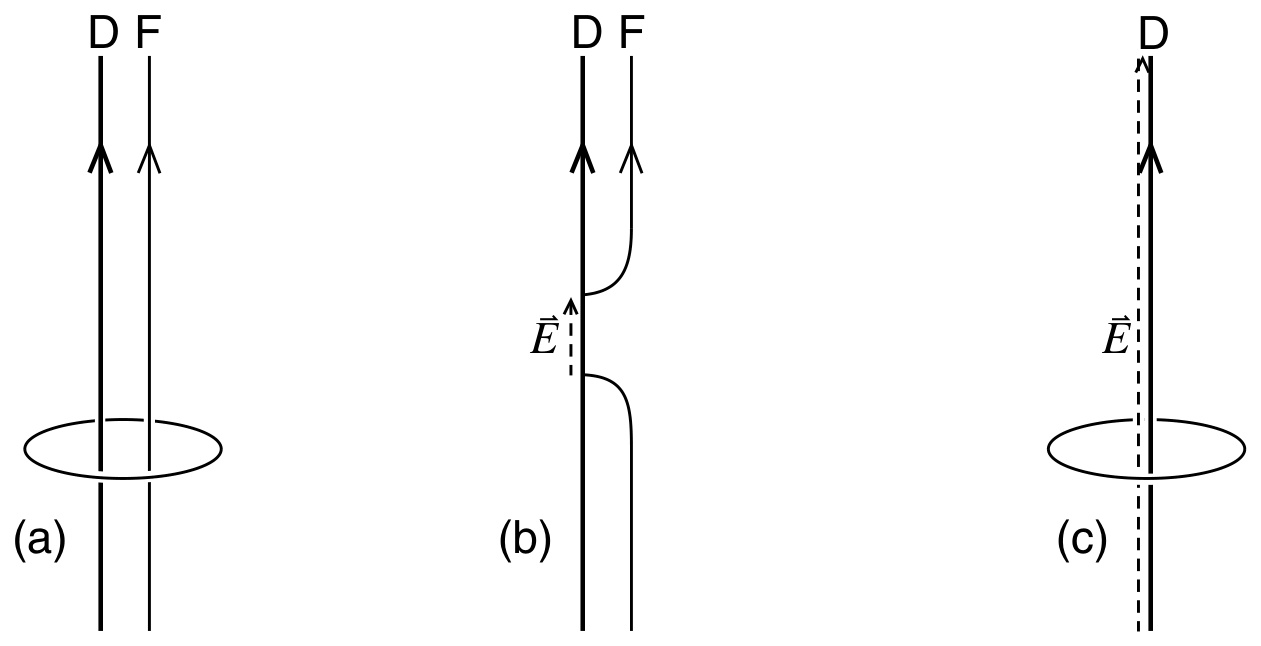
\includegraphics[width=0.75\textwidth]{figure/Fig13.5.jpg}
	\caption{(a) Parallel D-string and F-string. The loop signifies a 7-sphere surrounding the strings. (b) The F-string breaks, its ends attaching to the D-string. (c) Final state: D-string with flux.}
	\label{fig:13.5}
\end{figure}

However, the system can lower its energy as shown in Figure~\ref{fig:13.5}. The F-string breaks, with its endpoints attached to the D-string. The endpoints can then move off to infinity, leaving only the D-string behind. This cannot be the whole story because the F-string carries the NS--NS 2-form charge, as measured by the integral of $*H_{\textit{3}}$ over the 7-sphere in the figure: this flux must still be nonzero in the final configuration. This comes about because the F-string endpoints are charged under the D-string gauge field, so an electric flux runs between them. This flux remains in the end. Further, from the D-string action
\begin{equation}
	S_1 = -T_1\int \dif^2\xi\,\me^{-\Phi}\sqrt{-\det(G_{ab} + B_{ab} + 2\pi\alpha' F_{ab})} \:, \label{13.6.7}
\end{equation}
one sees that $B_{\mu\nu}$ has a source proportional to the invariant electric flux $\mathcal{F}_{ab} = F_{ab} + B_{ab}/(2\pi\alpha')$ on the D-string.

The simplest way to see that the resulting state is supersymmetric is via T-duality along the 1-direction. The D1-brane becomes a D0-brane. The electric field is T-dual to a velocity, $\dot{A}_1 \to \dot{X}^1/(2\pi\alpha')$, so the T-dual state is a D0-brane moving with constant velocity. This is invariant under the same number of supersymmetries as a D-brane at rest, namely the Lorentz boost of those supersymmetries. The boosted supersymmetries are linear combinations of the unbroken and broken supersymmetries of the D0-brane at rest. All of this carries over by T-duality to the D1--F1 system. We leave it as an exercise to verify that the tension takes the BPS value.

The F-string `dissolves' in the D-string, leaving flux behind. For separated D- and F-strings there is an attractive force at long distance, a consequence of the lack of supersymmetry. One might have expected that the binding energy would be of order $g$, the typical scale for D-brane processes, but the binding tension
\begin{equation}
	\tau_{(1,0)} + \tau_{(0,1)} - \tau_{(1,1)} = \frac{1 - \mathcal{O}(g)}{2\pi\alpha'} \label{13.6.8}
\end{equation}
is almost the total tension of the F-string.
\begin{tcolorbox}[breakable]
	\begin{remark}
		\textit{\eqref{13.6.4}--\eqref{13.6.8}.} With $\tau_{(1,0)}=1/2\pi\alpha'$ and $\tau_{(0,1)}=1/2\pi\alpha'g$,
		\begin{align*}
			2\pi\alpha'\tau_{(1,1)} = (g^{-2}+1)^{1/2} = g^{-1}(1+g^2)^{1/2} \eqs{1} g^{-1}+\frac g2-\frac{g^3}{8}+\cdots,\\
			2\pi\alpha'\bigl(\tau_{(1,0)}+\tau_{(0,1)}-\tau_{(1,1)}\bigr) = 1-\frac g2+\mathcal O(g^3) .
		\end{align*}
		At (1), $(1+x)^{1/2}=1+\frac x2-\frac{x^2}8+\cdots$. The binding energy is the whole F-string tension up to $\mathcal O(g)$: for $g\to0$ the bound F-string costs only the energy $\frac{g}{2}\cdot\frac1{2\pi\alpha'}$ of the electric flux on the heavy D-string.

		\textit{The exercise: the tension of the D-string with flux.} Take \eqref{13.6.7} with constant dilaton ($T_1e^{-\Phi}=\tau_1$), $B=0$, flat metric, and a constant electric field $F_{01}=E$ along the string. With $x=2\pi\alpha'E$, $-\det(\eta_{ab}+2\pi\alpha'F_{ab})=1-x^2$, and
		\begin{align*}
			\mathcal L &= -\tau_1(1-x^2)^{1/2},\qquad
			\Pi=\frac{\partial\mathcal L}{\partial E}=\frac{2\pi\alpha'\tau_1x}{(1-x^2)^{1/2}},\\
			\mathcal H &= \Pi E-\mathcal L \eqs{2} \frac{\tau_1}{(1-x^2)^{1/2}} \;\Longrightarrow\; \mathcal H^2 = \tau_1^2+\frac{\tau_1^2x^2}{1-x^2} = \tau_1^2+\Bigl(\frac{\Pi}{2\pi\alpha'}\Bigr)^2 .
		\end{align*}
		At (2), $\Pi E=\tau_1x^2/(1-x^2)^{1/2}$ and $x^2/(1-x^2)^{1/2}+(1-x^2)^{1/2}=(1-x^2)^{-1/2}$. The momentum $\Pi$ conjugate to $A_1$ is quantized in integers on a compact string, because large gauge transformations shift the holonomy of $A_1$ by $2\pi$. The endpoints of the F-strings are its unit charges, so $\Pi=p$ for $p$ dissolved F-strings. Then
		\begin{equation*}
			\mathcal H = \Bigl(\frac1{(2\pi\alpha'g)^2}+\frac{p^2}{(2\pi\alpha')^2}\Bigr)^{1/2} = \frac{(p^2+g^{-2})^{1/2}}{2\pi\alpha'} = \tau_{(p,1)} ,
		\end{equation*}
		exactly the BPS value \eqref{13.6.3} with $q=1$. The T-dual statement is the relativistic energy $\tau_0/(1-v^2)^{1/2}$ of the moving D0-brane, with $v=2\pi\alpha'\dot A_1=x$.
	\end{remark}
\end{tcolorbox}

String theory with a constant open string field strength has a simple worldsheet description. The variation of the worldsheet action includes a surface term:
\begin{equation}
	\int_{\del\mathcal{M}}\dif s\:\delta X^\mu\Bigl(\frac{1}{2\pi\alpha'}\del_n X_\mu + \mi F_{\mu\nu}\del_t X^\nu\Bigr) \:, \label{13.6.9}
\end{equation}
implying the linear boundary condition:
\begin{equation}
	\del_n X^\mu + 2\pi\alpha'\mi F^{\mu\nu}\del_t X_\nu = 0 \:. \label{13.6.10}
\end{equation}
\begin{tcolorbox}[breakable]
	\begin{remark}
		\textbf{Conventions.} Euclidean world-sheet action $S=\frac{1}{4\pi\alpha'}\int_{\mathcal M}\dif^2\sigma\,\partial_aX^\mu\partial_aX_\mu-\mi\int_{\partial\mathcal M}\dif s\,A_\mu\partial_tX^\mu$, where the boundary coupling is the Wilson line for a charge at the string endpoint. $\partial_n$ and $\partial_t$ are the normal and tangential derivatives, and the orientation signs are those of the text.

		\textit{The surface term.} Varying the bulk term and integrating by parts leaves the boundary piece $\frac{1}{2\pi\alpha'}\int\dif s\,\delta X^\mu\partial_nX_\mu$. For the Wilson line,
		\begin{align*}
			\delta\int\dif s\,A_\mu\partial_tX^\mu &= \int\dif s\bigl(\partial_\nu A_\mu\,\delta X^\nu\,\partial_tX^\mu+A_\mu\partial_t\delta X^\mu\bigr)\\
			&\eqs{1} \int\dif s\,\delta X^\nu\bigl(\partial_\nu A_\mu-\partial_\mu A_\nu\bigr)\partial_tX^\mu = \int\dif s\,\delta X^\nu F_{\nu\mu}\partial_tX^\mu .
		\end{align*}
		At (1), $A_\mu\partial_t\delta X^\mu$ was integrated by parts along the closed boundary, and $\partial_tA_\mu=\partial_\nu A_\mu\,\partial_tX^\nu$. So $-\mi\times$ this, relabelled, together with the bulk piece gives the total surface term \eqref{13.6.9}, $\int\dif s\,\delta X^\mu\bigl(\frac{1}{2\pi\alpha'}\partial_nX_\mu+\mi F_{\mu\nu}\partial_tX^\nu\bigr)$, up to the overall orientation sign. For $\delta X^\mu$ free on the boundary (Neumann directions of the D-brane), the bracket must vanish; multiplying by $2\pi\alpha'$ and raising the index gives \eqref{13.6.10}. Only the gauge-invariant $F$ appears. The condition interpolates linearly between Neumann ($F=0$) and, as $F\to\infty$, Dirichlet ($\partial_tX=0$), which is the world-sheet version of the T-duality between flux and tilted branes.
	\end{remark}
\end{tcolorbox}

All of the above extends immediately to $p$ F-strings and one D-string forming a supersymmetric $(p,1)$ bound state. The general case of $p$ F-strings and $q$ D-strings is more complicated because the gauge dynamics on the D-strings is non-Abelian. A two-dimensional gauge coupling has units of inverse length-squared: $g_{\mathrm{D}1}^2 = g/(2\pi\alpha')$. For dynamics on length scale $l$ the effective dimensionless coupling is $g l^2/(2\pi\alpha')$. No matter how weak the underlying string coupling $g$, the D-string dynamics at long distances is strongly coupled.

Focus for example on two D-strings and one F-string. There is a state with a separated $(1,1)$ bound state and $(0,1)$ D-string. The tension
\begin{equation}
	\tau_{(1,1)} + \tau_{(0,1)} = \frac{(g^{-2} + 1)^{1/2} + g^{-1}}{2\pi\alpha'} = \frac{2g^{-1} + g/2 + \mathcal{O}(g^3)}{2\pi\alpha'} \label{13.6.11}
\end{equation}
exceeds the BPS bound
\begin{equation}
	\tau_{(1,2)} = \frac{(4g^{-2} + 1)^{1/2}}{2\pi\alpha'} = \frac{2g^{-1} + g/4 + \mathcal{O}(g^3)}{2\pi\alpha'} \:. \label{13.6.12}
\end{equation}
The electric flux is on the first D-brane, so as a $\mathrm{U}(2)$ matrix this is proportional to:
\begin{equation}
	\begin{pmatrix} 1 & 0 \\ 0 & 0 \end{pmatrix} = \frac{1}{2}\begin{pmatrix} 1 & 0 \\ 0 & 1 \end{pmatrix} + \frac{1}{2}\begin{pmatrix} 1 & 0 \\ 0 & -1 \end{pmatrix} \:. \label{13.6.13}
\end{equation}
We have separated this into $\mathrm{U}(1)$ and $\mathrm{SU}(2)$ pieces. When we bring the two D-strings together, the $\mathrm{SU}(2)$ field becomes strongly coupled but the $\mathrm{U}(1)$ part remains free. If the $\mathrm{SU}(2)$ part is screened by the massless fields on the D-strings, then the total energy in the flux is reduced by a factor of 2, from \eqref{13.6.11} to the BPS value \eqref{13.6.12}.
\begin{tcolorbox}[breakable]
	\begin{remark}
		\textit{Expansions.} With $(1+x)^{1/2}=1+\frac x2+\cdots$,
		\begin{align*}
			(g^{-2}+1)^{1/2}+g^{-1} &= 2g^{-1}+\frac g2+\mathcal O(g^3),\\
			(4g^{-2}+1)^{1/2} &= 2g^{-1}\Bigl(1+\frac{g^2}{4}\Bigr)^{1/2} = 2g^{-1}+\frac g4+\mathcal O(g^3),
		\end{align*}
		which are \eqref{13.6.11} and \eqref{13.6.12}. The rest-energy $2g^{-1}/2\pi\alpha'$ of the two D-strings is common, and the flux energy is $\frac{g}{2}$ versus $\frac g4$ in units of $1/2\pi\alpha'$.

		\textit{Why the factor is 2.} At weak coupling the flux energy is the electric energy $\frac{g_{\rm D1}^2}{2}\operatorname{Tr}(\Pi^2)$ of the D-string gauge theory per unit length, the analogue of $\frac12E^2$. For unit flux on one of two strings, $\Pi=\mathrm{diag}(1,0)$ and $\operatorname{Tr}\Pi^2=1$. After screening of the SU(2) part only the U(1) part $\frac12\mathbb 1$ of \eqref{13.6.13} remains, with $\operatorname{Tr}(\frac12\mathbb 1)^2=\frac12$. The ratio $\frac12$ is exactly $(g/4)/(g/2)$. The same check with $g_{\rm D1}^2=g/2\pi\alpha'$ fixes the absolute value: for one string $\frac{g}{2\cdot2\pi\alpha'}$, matching $\tau_{(1,1)}-\tau_{(0,1)}$ at order $g$.
	\end{remark}
\end{tcolorbox}

Focus on four of the 16 supersymmetries, forming the equivalent of $d = 4, N = 1$ supersymmetry. The six scalars $X^{4,\dots,9}$ can be written as three chiral superfields $\Phi^i$, with the potential coming from a superpotential $\operatorname{Tr}(\Phi^1[\Phi^2,\Phi^3])$. Adding a mass term to the superpotential:
\begin{equation}
	W(\Phi) = \operatorname{Tr}(\Phi^1[\Phi^2,\Phi^3]) + m\operatorname{Tr}(\Phi^i\Phi^i) \label{13.6.14}
\end{equation}
breaks the gauge group to $\mathrm{SU}(2)$ and lifts the flat directions. Its mass cannot depend on $m$ by the BPS property. Increasing $m$ reduces the effective dimensionless coupling $g/(2\pi\alpha' m^2)$ to a value where the system becomes weakly coupled, establishing the existence of the supersymmetric $(p,q)$ bound string for all coprime $p$ and $q$.

\subsection*{D0--D$p$ BPS Bounds}

For a system with the charges of a D0-brane and a D$p$-brane extended in the $(1,\dots,p)$-directions, the supersymmetry algebra becomes
\begin{equation}
	\frac{1}{2}\begin{Bmatrix} Q_\alpha \\ \tilde{Q}_\alpha \end{Bmatrix}\begin{Bmatrix} Q_\beta^\dagger & \tilde{Q}_\beta^\dagger \end{Bmatrix} = M\begin{pmatrix} 1 & 0 \\ 0 & 1 \end{pmatrix}\delta_{\alpha\beta} + \begin{pmatrix} 0 & Z \\ -Z^\dagger & 0 \end{pmatrix}(\Gamma^0)_{\alpha\beta} \:, \label{13.6.15}
\end{equation}
where
\begin{equation}
	Z = \tau_0 + \tau_p V_p\beta \:, \quad \beta = \beta_1\cdots\beta_p \:. \label{13.6.16}
\end{equation}
We have wrapped the D$p$-brane on a torus of volume $V_p$ so that its mass will be finite. The positivity of the left-hand side implies that
\begin{subequations} \label{13.6.17}
	\begin{align}
		M^2\begin{pmatrix} 1 & 0 \\ 0 & 1 \end{pmatrix} &\ge \begin{pmatrix} 0 & Z \\ -Z^\dagger & 0 \end{pmatrix}\Gamma^0\begin{pmatrix} 0 & Z \\ -Z^\dagger & 0 \end{pmatrix}\Gamma^0 = \begin{pmatrix} ZZ^\dagger & 0 \\ 0 & Z^\dagger Z \end{pmatrix} \:, \label{13.6.17a} \\
		ZZ^\dagger &= \tau_0^2 + \tau_0\tau_p V_p(\beta + \beta^\dagger) + \tau_p^2 V_p^2\beta\beta^\dagger \:. \label{13.6.17b}
	\end{align}
\end{subequations}

For $p$ a multiple of 4, $\beta$ is Hermitian and $\beta^2 = 1$. The BPS bound is then
\begin{equation}
	M \ge \tau_0 + \tau_p V_p \:. \label{13.6.18}
\end{equation}
For $p = 4k + 2$, $\beta$ is anti-Hermitian, $\beta^2 = -1$, and the BPS bound is
\begin{equation}
	M \ge \bigl(\tau_0^2 + \tau_p^2 V_p^2\bigr)^{1/2} \:. \label{13.6.19}
\end{equation}
These bounds are consistent with our earlier results on supersymmetry breaking, noting that $\#\mathrm{ND} = p$. For $p = 4k$, a separated 0-brane and $p$-brane saturate the BPS bound \eqref{13.6.18}. For $p = 4k + 2$ they do not saturate the bound and so cannot be in a BPS state.
\begin{tcolorbox}[breakable]
	\begin{remark}
		\textbf{Conventions.} Majorana basis, so $\Gamma^0$ is real antisymmetric ($\Gamma^{0\dagger}=-\Gamma^0$) and each $\beta_m$ is real orthogonal; $\beta=\beta_1\cdots\beta_p$ with $p$ even. Write $K=\begin{pmatrix}0&Z\\-Z^\dagger&0\end{pmatrix}\Gamma^0$ for the second term of \eqref{13.6.15}.

		\textit{$K$ is Hermitian with a symmetric spectrum.} $\Gamma^0$ commutes with the spatial $\beta_m$ (box after \eqref{13.2.10}), hence with $Z$ and $Z^\dagger$. Then $(Z\Gamma^0)^\dagger=\Gamma^{0\dagger}Z^\dagger=-Z^\dagger\Gamma^0$, so the off-diagonal blocks of $K$ are adjoints of each other and $K$ is Hermitian. Also $\sigma_3K\sigma_3=-K$ with $\sigma_3=\mathrm{diag}(1,-1)$ in the $(Q,\tilde Q)$ index, so the eigenvalues of $K$ come in pairs $\pm\kappa$. Positivity of $M+K$ therefore means $M\ge|\kappa|$ for every eigenvalue, i.e.\ $M^2\ge K^2$:
		\begin{align*}
			K^2 = \begin{pmatrix}0&Z\\-Z^\dagger&0\end{pmatrix}^2(\Gamma^0)^2 \eqs{1} -\begin{pmatrix}-ZZ^\dagger&0\\0&-Z^\dagger Z\end{pmatrix} = \begin{pmatrix}ZZ^\dagger&0\\0&Z^\dagger Z\end{pmatrix},
		\end{align*}
		where (1) uses $[\Gamma^0,Z]=0$ and $(\Gamma^0)^2=-1$. This is \eqref{13.6.17a}, and expanding $ZZ^\dagger$ with $Z=\tau_0+\tau_pV_p\beta$ gives \eqref{13.6.17b}.

		\textit{Hermiticity of $\beta$.} Since $\beta$ is real orthogonal, $\beta^\dagger=\beta^{\mathrm T}=\beta^{-1}$, and by the computation \eqref{bsq} with $p$ factors,
		\begin{gather*}
			\beta^2=(-1)^{p(p+1)/2}=\begin{cases}+1 & p=4k,\\ -1 & p=4k+2,\end{cases}\\
			\beta^\dagger=\beta^{-1}=\begin{cases}+\beta & p=4k \ (\text{Hermitian}),\\ -\beta & p=4k+2 \ (\text{anti-Hermitian}).\end{cases}
		\end{gather*}
		For $p=4k$: $p(p+1)/2=2k(4k+1)$ is even. For $p=4k+2$: $(2k+1)(4k+3)$ is odd.

		\textit{The bounds.} With $\beta\beta^\dagger=1$:
		\begin{align*}
			p=4k:&\quad ZZ^\dagger=\tau_0^2+2\tau_0\tau_pV_p\,\beta+\tau_p^2V_p^2,\ \ \beta=\pm1\text{ on eigenvectors}\\ &\quad\;\Longrightarrow\; M^2\ge(\tau_0+\tau_pV_p)^2,\\
			p=4k+2:&\quad \beta+\beta^\dagger=0 \;\Longrightarrow\; ZZ^\dagger=\tau_0^2+\tau_p^2V_p^2 \;\Longrightarrow\; M^2\ge\tau_0^2+\tau_p^2V_p^2 ,
		\end{align*}
		which are \eqref{13.6.18} and \eqref{13.6.19}. Since $\#\mathrm{ND}=p$ for D0--D$p$, this matches the box after the $\#\mathrm{ND}$ list. For $p=4,8$ the separated branes have $M=\tau_0+\tau_pV_p$, saturate the bound, and preserve 8 supercharges (the $\beta=+1$ eigenspace). For $p=2,6$ they have $M=\tau_0+\tau_pV_p>(\tau_0^2+\tau_p^2V_p^2)^{1/2}$ and break all supersymmetry.
	\end{remark}
\end{tcolorbox}

\subsection*{D0--D0 Bound States}

The BPS bound for the quantum numbers of two 0-branes is $2\tau_0$, so any bound state will be at the lower edge of the continuous spectrum of two-body states. Nevertheless there is a well-defined question as to whether a normalizable state of energy $2\tau_0$ exists.

Compactify the 9-direction and add one unit of compact momentum, $p^9 = 1/R$. In a two-body state this momentum must be carried by one 0-brane or the other for minimum energy:
\begin{equation}
	E \approx \tau_0 + \Bigl(\tau_0 + \frac{(p^9)^2}{2\tau_0}\Bigr) = 2\tau_0 + \frac{1}{2\tau_0 R^2} \:. \label{13.6.20}
\end{equation}
For a bound state of mass $2\tau_0$, on the other hand, the minimum energy is
\begin{equation}
	E \approx 2\tau_0 + \frac{(p^9)^2}{4\tau_0} = 2\tau_0 + \frac{1}{4\tau_0 R^2} \:, \label{13.6.21}
\end{equation}
a finite distance below the continuum states. The reader may note some resemblance between these energies and the earlier \eqref{13.6.11} and \eqref{13.6.12}. In fact the two systems are T-dual to one another. Taking the T-dual along the 9-direction, the D0-branes become D1-branes and the unit of momentum becomes a unit of fundamental string winding to give the $(1,2)$ system, now at finite radius $R' = \alpha'/R$. Quantizing the $(1,2)$ string at finite $R'$ one finds that the minimum energy is indeed \eqref{13.6.21}.
\begin{tcolorbox}[breakable]
	\begin{remark}
		\textit{\eqref{13.6.20}--\eqref{13.6.21}.} In the nonrelativistic limit a particle of mass $m$ with momentum $p^9$ has $E\approx m+(p^9)^2/2m$. Putting $p^9=1/R$ on one D0-brane gives $m=\tau_0$, hence $2\tau_0+1/2\tau_0R^2$. Putting it on the bound state of mass $2\tau_0$ gives $2\tau_0+1/4\tau_0R^2$, lower by $1/4\tau_0R^2$.

		\textit{The T-dual check.} Under T-duality along $x^9$, $R'=\alpha'/R$ and $g'=g\alpha'^{1/2}/R$. A D0-brane becomes a D-string wrapped once on the dual circle, and the momentum becomes one unit of F-string winding:
		\begin{align*}
			2\pi R'\,\tau'_{\rm D1} = \frac{2\pi R'}{2\pi\alpha'g'} \eqs{1} \frac{1}{g\alpha'^{1/2}} = \tau_0,\qquad
			2\pi R'\,\tau_{\rm F1} = \frac{R'}{\alpha'} = \frac1R .
		\end{align*}
		At (1), $R'/(\alpha'g')=R'R/(g\alpha'^{3/2})=1/(g\alpha'^{1/2})$ using $RR'=\alpha'$. The $(p,q)$ tensions below are those of \eqref{13.6.3} with the dual coupling $g'$. So the two systems have the same charges, and their energies are the $(p,q)$ tensions times $2\pi R'$:
		\begin{align*}
			(1,1)+(0,1):&\quad 2\pi R'\bigl(\tau_{(1,1)}+\tau_{(0,1)}\bigr)=\Bigl(\tau_0^2+\frac1{R^2}\Bigr)^{1/2}+\tau_0 \approx 2\tau_0+\frac{1}{2\tau_0R^2},\\
			(1,2):&\quad 2\pi R'\,\tau_{(1,2)}=\Bigl(4\tau_0^2+\frac1{R^2}\Bigr)^{1/2}\approx 2\tau_0+\frac{1}{4\tau_0R^2},
		\end{align*}
		using $(A^2+x)^{1/2}\approx A+x/2A$. These are \eqref{13.6.20} and \eqref{13.6.21}. The $(1,2)$ bound string of \eqref{13.6.12} is the T-dual of the D0--D0 bound state with one unit of momentum.
	\end{remark}
\end{tcolorbox}

Taking $R \to \infty$ the energy of the bound state approaches the continuum, but the wavefunction remains normalizable. For $m$ D0-branes and $n$ units of momentum, the bound state exists whenever $\gcd(m,n) = 1$. The degeneracy of supersymmetric bound states is
\begin{equation}
	D_{mn} = \sum_{d|\gcd(m,n)} \frac{1}{d^2} \:. \label{13.6.24}
\end{equation}
For two D0-branes, there is a unique $L^2$-normalizable bound state.

\subsection*{D0--D2 Bound States}

For a D0-brane and a D2-brane, the relevant bound is \eqref{13.6.19}. A separated 0-brane and 2-brane have energy $\tau_0 + \tau_2 V_2 > (\tau_0^2 + \tau_2^2 V_2^2)^{1/2}$, so any bound state must be strictly below the continuum.

Use T-duality in the directions 1 and 2, but only half as much in the second as in the first, so that the 0-brane becomes a D-string wrapped in the 1-direction and the 2-brane becomes a D-string wrapped in the 2-direction. Now there is an obvious state with the same charges and lower energy, a single D-string running at an angle to wrap once in each direction. A single wrapped D-string is a BPS state (an ultrashort multiplet to be precise). Now use T-duality to return to the original description. As in Figure~\ref{fig:13.2}, this will be a D2-brane with a nonzero magnetic field, such that
\begin{equation}
	\int_{\mathrm{D}2} F_{\textit{2}} = 2\pi \:. \label{13.6.22}
\end{equation}
We can also check that this state has the correct R--R charges. From the Chern--Simons action \eqref{13.3.18}, the coupling of the magnetized 2-brane to $C_{\textit{1}}$ is
\begin{equation}
	2\pi\alpha'\mu_2\int_{\mathrm{D}2} F_{\textit{2}} = 4\pi^2\alpha'\mu_2 = \mu_0 \:, \label{13.6.23}
\end{equation}
which is indeed one unit of 0-brane charge. The energy of the magnetized D2-brane from the DBI action is
\begin{equation}
	E = T_2\int \dif^2\xi\,\sqrt{1 + (2\pi\alpha' F_{12})^2} = \sqrt{\tau_0^2 + \tau_2^2 V_2^2} \:,
\end{equation}
which precisely saturates the BPS bound \eqref{13.6.19}.
\begin{tcolorbox}[breakable]
	\begin{remark}
		\textbf{Conventions.} Constant dilaton, so $T_2e^{-\Phi}=\tau_2$; the text's $T_2$ in the energy formula should be read as $\tau_2$ for the physical energy. The flux is uniform, $F_{12}=2\pi/V_2$. From \eqref{13.3.7}, $\mu_{p-1}/\mu_p=\tau_{p-1}/\tau_p=2\pi\alpha'^{1/2}$.

		\textit{Flux quantization \eqref{13.6.22}.} A D-string wrapping once around each of the two cycles of the torus is T-dual (Figure~\ref{fig:13.2}) to a D2-brane whose magnetic field gives total flux one quantum. With U(1) gauge transformations of period $2\pi$, that quantum is $\int F_2=2\pi$.

		\textit{Charge \eqref{13.6.23}.} The $F\wedge C_1$ term of \eqref{13.3.18} is $\mu_2\int2\pi\alpha'F_2\wedge C_1$. For constant $C_1$ this is $2\pi\alpha'\mu_2\cdot2\pi\int C_1=4\pi^2\alpha'\mu_2\int C_1$, and $4\pi^2\alpha'\mu_2=(2\pi\alpha'^{1/2})^2\mu_2=\mu_0$.

		\textit{Energy.} For a static magnetic field only $F_{12}$ is nonzero, and $-\det(\eta_{ab}+2\pi\alpha'F_{ab})=\det\begin{pmatrix}1&x\\-x&1\end{pmatrix}=1+x^2$ with $x=2\pi\alpha'F_{12}$. So
		\begin{align*}
			E = \tau_2\int\dif^2\xi\,(1+x^2)^{1/2} = \tau_2V_2\Bigl(1+\frac{(4\pi^2\alpha')^2}{V_2^2}\Bigr)^{1/2} \eqs{1} \bigl(\tau_2^2V_2^2+\tau_0^2\bigr)^{1/2},
		\end{align*}
		where (1) uses $4\pi^2\alpha'\tau_2=\tau_0$. This equals the bound \eqref{13.6.19}, so the magnetized D2-brane is the BPS D0--D2 bound state. The binding energy $\tau_0+\tau_2V_2-(\tau_0^2+\tau_2^2V_2^2)^{1/2}$ is positive. For large $V_2$ it is $\approx\tau_0-\tau_0^2/2\tau_2V_2$: the D0-brane has spread out into flux and costs almost no energy.
	\end{remark}
\end{tcolorbox}

\subsection*{D0--D4 Bound States and Gauge Instantons}

Now consider the D0--D4 system. For one D0-brane and one D4-brane, the separated state saturates the BPS bound \eqref{13.6.18}. The states of the system have a simple counting. The 0-brane can be placed anywhere on the 4-brane, so its center-of-mass motion gives the usual $2^8$ states of a $d = 6$ superparticle delocalized on the D4-brane. The fermion in the 0-4 hypermultiplet has eight real components (the smallest spinor in six dimensions) and their zero modes generate $2^4$ ground states localized on the D0-brane. The tensor product gives the $2^{12}$ states.

For two D0-branes and one D4-brane, one gets the correct count as follows. We can have the two D0-branes bound to the D4-brane independently of one another; for a large D4-brane their interactions can be neglected. Each D0-brane has $2^4$ states as noted above, eight bosonic and eight fermionic. Now count the symmetric product of these states, as appropriate for identical particles (the statistics of D0-branes is discussed in section 14.3). The symmetric product of two eight-state representations has $(8 \times 9)/2 = 36$ states, while the antisymmetric product of two eight-state representations has $(8 \times 7)/2 = 28$ states. The total number of states is $(36 + 28) \times 2^8 = 2^{14}$. This matches the counting of threshold bound states.

\paragraph*{D-branes as instantons}:
The D0--D4 system is interesting in other ways. Consider its scalar potential:
\begin{equation}
	V(\chi, X) = \frac{g_{\mathrm{D}0}^2}{4}\sum_{A=1}^3(\chi_i^\dagger\sigma_{ij}^A\chi_j)^2 + \sum_{i=1}^5\frac{(X^i - X'^i)^2}{2\pi\alpha'}\chi^\dagger\chi \:. \label{13.6.25}
\end{equation}
The second term by itself has two branches of zeros:
\begin{equation}
	X^i - X'^i = 0 \:, \quad \chi \neq 0 \label{13.6.26}
\end{equation}
and
\begin{equation}
	X^i - X'^i \neq 0 \:, \quad \chi = 0 \:. \label{13.6.27}
\end{equation}
The first of these, where the hypermultiplet scalars are nonzero, is known as a \textbf{Higgs branch}. The second, where the vector multiplet scalars (the collective coordinates) are nonzero, is known as a \textbf{Coulomb branch}. In the present case the first term in the potential, the D-term, eliminates the Higgs branch for a single D4-brane: the condition
\begin{equation}
	D^A \equiv \chi_i^\dagger\sigma_{ij}^A\chi_j = 0 \label{13.6.28}
\end{equation}
implies that $\chi = 0$. However, for two D4-branes $\chi$ acquires a D4-brane index $a = 1, 2$ and the D-term condition becomes:
\begin{equation}
	\chi_{ia}^\dagger\sigma_{ij}^A\chi_{ja} = 0 \:. \label{13.6.29}
\end{equation}
This is solved by
\begin{equation}
	\chi_{ia} = v\delta_{ia} \label{13.6.30}
\end{equation}
for any $v$, or more generally
\begin{equation}
	\chi_{ia} = v U_{ia} \label{13.6.31}
\end{equation}
for any constant $v$ and unitary $U \in \mathrm{SU}(2)$.
\begin{tcolorbox}[breakable]
	\begin{remark}
		\textbf{Conventions.} $\chi_{ia}$ has an SU(2)$_R$ doublet index $i$ and a D4-brane index $a$; regard it as a matrix $\chi$ with rows $i$ and columns $a$. The Pauli matrices obey $\sum_A\sigma^A_{ij}\sigma^A_{kl}=2\delta_{il}\delta_{kj}-\delta_{ij}\delta_{kl}$.

		\textit{A note on \eqref{13.6.25}.} By \eqref{13.5.24}, the stretching term is $\bigl((X^i-X'^i)/2\pi\alpha'\bigr)^2\chi^\dagger\chi$, i.e.\ it has $(2\pi\alpha')^2$ in the denominator; the printed $2\pi\alpha'$ is not dimensionally consistent with a mass term. The D-term coefficient $g_{\rm D0}^2/4$ also differs from the $g^2/2$ in \eqref{13.5.21}. This only rescales the D-term and does not affect the zero sets below.

		\textit{One D4-brane.} For a single doublet, the Fierz identity gives
		\begin{equation*}
			\sum_A\bigl(\chi^\dagger\sigma^A\chi\bigr)^2 = \sum_A\chi^*_i\sigma^A_{ij}\chi_j\,\chi^*_k\sigma^A_{kl}\chi_l \eqs{1} 2(\chi^\dagger\chi)^2-(\chi^\dagger\chi)^2 = (\chi^\dagger\chi)^2 ,
		\end{equation*}
		where (1) uses the completeness relation. So $D^A=0$ for all $A$ forces $\chi^\dagger\chi=0$, i.e.\ $\chi=0$. There is no Higgs branch.

		\textit{Two D4-branes.} Now $D^A=\sum_a\chi^*_{ia}\sigma^A_{ij}\chi_{ja}=\operatorname{tr}\bigl(\sigma^A\chi\chi^\dagger\bigr)$. The Hermitian $2\times2$ matrix $\chi\chi^\dagger$ has vanishing traceless part if and only if $D^A=0$ for all three $A$, so
		\begin{equation*}
			\chi\chi^\dagger = |v|^2\,\mathbb 1 \;\Longleftrightarrow\; \chi = vU,\quad U\in\mathrm U(2) .
		\end{equation*}
		The overall phase of $U$ can be absorbed into $v$, leaving $U\in\mathrm{SU}(2)$, which gives \eqref{13.6.30}--\eqref{13.6.31}. Counting: $\chi$ has $2\times2$ complex $=8$ real components. The 3 conditions $D^A=0$ and the U(1) gauge symmetry of the single D0-brane remove 4, leaving 4 real moduli: $|v|$ and $U\in\mathrm{SU}(2)$ (3 parameters). Together with the 4 positions of the D0-brane along the D4-branes, this gives 8, the dimension of the moduli space of one SU(2) instanton: 4 positions, 1 scale size $\rho\leftrightarrow|v|$, and 3 gauge orientations.
	\end{remark}
\end{tcolorbox}

On the Coulomb branch the D0-brane is at some separation $X^i - X'^i$ from the D4-brane, describing the states of a separated D0-brane and D4-brane. But on the Higgs branch, the D0-brane has dissolved into a gauge instanton.

Recall that non-Abelian gauge theories in four Euclidean dimensions have classical solutions, \textbf{instantons}, that are localized in all four dimensions. Their distinguishing property is that the field strength is self-dual or anti-self-dual:
\begin{equation}
	*F_{\textit{2}} = \pm F_{\textit{2}} \:, \label{13.6.32}
\end{equation}
so that the Bianchi identity implies the field equations. Because the classical theory is scale-invariant, the characteristic size of the configuration is undetermined --- there is a family of solutions parameterized by scale size $\rho$. The $\mathrm{U}(n)$ gauge theory on coincident D4-branes is five-dimensional, so a configuration that looks like an instanton in the four spatial dimensions and is independent of time is a static classical solution, a soliton.

This soliton has many properties in common with the D0-brane bound to the D4-branes:
\begin{enumerate}
	\item First, it is a BPS state, breaking half of the supersymmetries of the D4-branes. The supersymmetry variation of the gaugino is
	\begin{equation}
		\delta\lambda \propto F_{MN}\Gamma^{MN}\zeta \:. \label{13.6.33}
	\end{equation}
	Here the nonzero terms involve the components of $\Gamma^{MN}$ in the spatial directions of the D4-brane, which are generators of $\mathrm{SO}(4) = \mathrm{SU}(2)\times\mathrm{SU}(2)$. The self-duality relation \eqref{13.6.32} amounts to the statement that only the generators of the first or second $\mathrm{SU}(2)$ appear in the variation. The ten-dimensional spinor $\zeta$ decomposes into
	\begin{equation}
		(\mathbf{4}, \mathbf{2}, \mathbf{1}) + (\mathbf{4}, \mathbf{1}, \mathbf{2}) \label{13.6.34}
	\end{equation}
	under $\mathrm{SO}(5,1)\times\mathrm{SU}(2)\times\mathrm{SU}(2)$, so half the components are invariant under each $\mathrm{SU}(2)$ and half the supersymmetry variations \eqref{13.6.33} are zero.
	
	\item Second, it carries the same R--R charge as the D0-brane. Expanding the Chern--Simons action \eqref{13.3.18} gives the term:
	\begin{equation}
		\frac{1}{2}(2\pi\alpha')^2\mu_4\int C_{\textit{1}}\wedge \operatorname{Tr}(F_{\textit{2}}\wedge F_{\textit{2}}) \:. \label{13.6.35}
	\end{equation}
	The topological charge of the instanton is
	\begin{equation}
		\int_{\mathrm{D}4}\operatorname{Tr}(F_{\textit{2}}\wedge F_{\textit{2}}) = 8\pi^2 \:, \label{13.6.36}
	\end{equation}
	so the total coupling to a constant $C_{\textit{1}}$ is $(4\pi^2\alpha')^2\mu_4 = \mu_0$, exactly the charge of the D0-brane.
	
	\item Finally, the moduli \eqref{13.6.31} for the $\mathrm{SU}(2)$ Higgs branch match those of the $\mathrm{SU}(2)$ instanton, $v$ to the scale size $\rho$ and $U$ to the orientation of the instanton in the gauge group. There are eight real hypermultiplet scalars in $\chi$. The three D-term conditions and the gauge rotation each remove one to leave four moduli. There are also four additional 0-0 moduli for the position of the particle within the D4-branes.
\end{enumerate}
\begin{tcolorbox}[breakable]
	\begin{remark}
		\textbf{Conventions.} The D4-branes span $x^0$ and $x^{1,\dots,4}$. The instanton lives in $x^{1,\dots,4}$, whose rotation group is $\mathrm{SO}(4)=\mathrm{SU}(2)_L\times\mathrm{SU}(2)_R$. $F$ is Hermitian, and the instanton number is $k=\frac1{8\pi^2}\int\operatorname{Tr}_{\rm f}F\wedge F$, so $k=1$ gives \eqref{13.6.36}. The gauge action is $-\frac{1}{4g_{\rm D4}^2}\int\operatorname{Tr}_{\rm f}F_{MN}F^{MN}$ as in \eqref{13.3.26}.

		\textit{Half the supersymmetry (item 1).} The generators $\Gamma^{mn}$, $m,n\in\{1,\dots,4\}$, split into self-dual and anti-self-dual combinations $\Gamma^{mn}_\pm=\frac12(\Gamma^{mn}\pm\frac12\epsilon^{mnpq}\Gamma^{pq})$, which generate the two SU(2) factors. Each annihilates the spinors that are singlets of its own factor. For self-dual $F$ only one set appears, $F_{mn}\Gamma^{mn}=F_{mn}\Gamma^{mn}_+$, so $\delta\lambda=0$ for every $\zeta$ in the summand of \eqref{13.6.34} that is a singlet of that SU(2). That summand is 8 of the 16 components, so half the supersymmetries of the D4-branes are unbroken. Anti-self-dual $F$ preserves the other half, which is the instanton versus anti-instanton, or D0 versus anti-D0, choice.

		\textit{R--R charge (item 2).} The $F\wedge F$ term of \eqref{13.3.18} for $p=4$ is $\mu_4\int\frac12(2\pi\alpha')^2\operatorname{Tr}(F\wedge F)\wedge C_1$, which is \eqref{13.6.35}. For constant $C_1$ and $k=1$,
		\begin{equation*}
			\frac12(2\pi\alpha')^2\mu_4\cdot8\pi^2 = 16\pi^4\alpha'^2\mu_4 = (4\pi^2\alpha')^2\mu_4 \eqs{1} \mu_0 ,
		\end{equation*}
		where (1) uses $\mu_{p-1}/\mu_p=2\pi\alpha'^{1/2}$ from \eqref{13.3.7} four times. So an instanton of charge $k$ carries exactly $k$ units of D0 charge.

		\textit{Mass.} For a static purely magnetic field the energy is $\frac1{4g_{\rm D4}^2}\int\dif^4x\operatorname{Tr}F_{mn}F_{mn}$. Using $\operatorname{Tr}(F_{mn}\mp{*F}_{mn})^2\ge0$ with $({*F})_{mn}=\frac12\epsilon_{mnpq}F_{pq}$ and $\int\dif^4x\operatorname{Tr}F_{mn}{*F}_{mn}=2\int\operatorname{Tr}F\wedge F$,
		\begin{equation*}
			E \ge \frac{1}{4g_{\rm D4}^2}\Bigl|\int\dif^4x\operatorname{Tr}F_{mn}{*F}_{mn}\Bigr| = \frac{1}{2g_{\rm D4}^2}\cdot8\pi^2|k| \eqs{2} \frac{4\pi^2|k|}{4\pi^2g\alpha'^{1/2}} = |k|\,\tau_0 ,
		\end{equation*}
		with equality for (anti-)self-dual $F$. At (2), $g_{\rm D4}^2=(2\pi)^2g\alpha'^{1/2}$ from \eqref{13.3.25}, and $\tau_0=1/(g\alpha'^{1/2})$ from \eqref{13.3.23}. The soliton's mass equals the D0-brane tension as well as its charge, as the BPS property requires.
	\end{remark}
\end{tcolorbox}

The precise connection between the D0-brane and the instanton is this. When the scale size $\rho$ is large compared to the string scale, the low energy effective field theory on the D4-branes gives a good description of the instanton. However, as $\rho$ is reduced below the string length, this description is no longer accurate. Happily, the D0-brane picture provides a description that is accurate in the opposite limit: the point $v = 0$ where the Higgs and Coulomb branches meet is the zero-size instanton, and turning on the Higgs moduli expands the instanton: as in the D0--D2 case, the D0-brane is dissolving into flux. This picture also accounts for the absence of a Higgs branch for a single D4-brane because there are no instantons for $\mathrm{U}(1)$.

The gauge field of the small instanton can be measured directly using a slow D0-brane probe (or a D1-brane probe in the T-dual D5--D9 system). After integrating out the massive fields, the effective theory on moduli space displays the instanton gauge field, providing a physical realization of the Atiyah--Drinfeld--Hitchin--Manin (ADHM) construction of the general instanton solution.

Returning to the bound state problem, the system with $m$ D0-branes bound to $n$ D4-branes is equivalent to quantum mechanics on the moduli space of $m$ $\mathrm{SU}(n)$ instantons. The number of supersymmetric states is related to the topology of this space, giving the degeneracy $D_{mn}$ as in \eqref{13.6.24}.

\subsection*{D0--D6 and D0--D8 Bound Systems}

\paragraph*{D0--D6 bound states}:
The relevant bound is \eqref{13.6.19} and again any bound state would be below the continuum. However, the long-distance force is repulsive and the zero-point energy of coincident 0-6 NS strings is positive, so there is no sign of instability toward a supersymmetric state. One can give 0-brane charge to the 6-brane by turning on flux, but there is no configuration that has only these two charges and saturates the BPS bound. So there are no supersymmetric bound states.

\paragraph*{D0--D8 bound states}:
This system is complicated in a number of ways. The R--R fields of the D8-brane do not fall off with distance (it has codimension 1, like a planar source in $3+1$ dimensions). The total energy is infinite, and the dilaton diverges a finite distance from the D8-brane. Thus the D8-brane cannot exist as an independent object, but only in connection with orientifold planes such as arise in the T-dual of the Type I theory.

